\documentclass[TS]{sesamanuel}

% modifications dans la classe (fichier sesamanuel.cls) :
% 	voir manuel 6e

%%%%%%%
%Rajouté le 12/06/2018 SV et BN pour compilation espace insécable sous linux 
%\DeclareUnicodeCharacter{00A0}{~} %pour remplacer les espaces insécables
%\DeclareUnicodeCharacter{2011}{-}
%\usepackage{pdfpages}
%%%%%%%


% a priori, après l'impression du livre, tout ce fichier devrait être
% fusionné avec la classe principale, dernière version

\AtBeginDocument{\color{Noir}}

\renewcommand*\StringPrerequis{Connaissances
  n\'ecessaires \`a ce chapitre}

\usepackage{textcomp,pgfplots}
% standalone ne gère pas graphicspath... hum...
\newcommand{\standalonepath}[1]{#1}
% Au début de chaque chapitre on redéfinira cette commande en
% indiquant le chemin

\frenchbsetup{og=«,fg=»,}

\renewcommand\PrefixeCorrection{Corrections/}
\DeclareRemLike{intuition}{Idée intuitive}
\DeclareRemLike{exemples}{Exemples}


\newcommand*\StringExemples{Exemples}
\makeatletter
\newcommand*\smc@cartoucheexemples{% au pluriel
  \begin{pspicture}(-\ExempleVRuleWidthFrame,0)
                 (\ExempleWidthFrame,\ExempleHeightFrame)
    \psframe*[linewidth=0pt,linecolor=ExempleEdgeFrameColor]
             (-\ExempleVRuleWidthFrame,-\ExempleHRuleWidthFrame)
             (\ExempleWidthFrame,\ExempleHeightFrame)
    \psframe*[linewidth=0pt,linecolor=ExempleBkgFrameColor]
             (0mm,-0mm)(\ExempleWidthFrame,\ExempleHeightFrame)
    \rput[B](\dimexpr\ExempleWidthFrame/2,0){%
      \ExempleTitleFont
      \textcolor{ExempleTitleColor}{\StringExemples}%
    }
  \end{pspicture}%
}

\newenvironment{exemples*1}[1][]{%
  \par\addvspace{\BeforeExempleVSpace}
  \let\correction\smc@one@exemplecorrection
  \let\itemize\smc@exempleitemize
  \let\enditemize\endsmc@exempleitemize
  \let\colitemize\smc@exemplecolitemize
  \let\endcolitemize\endsmc@exemplecolitemize
  \let\enumerate\smc@exempleenumerate
  \let\endenumerate\endsmc@exempleenumerate
  \let\colenumerate\smc@exemplecolenumerate
  \let\endcolenumerate\endsmc@exemplecolenumerate
  \let\partie\smc@nopartie
  \let\exercice\smc@noexercice
  \let\endexercice\endsmc@noexercice
  \let\corrige\smc@nocorrige
  \let\endcorrige\endsmc@nocorrige
  \def\smc@currpart{Exemple}%
  \hspace*{\dimexpr \SquareWidth*3}%
  \color{ExempleRuleColor}%
  \vrule width \RuleWidth
  \hspace*{\dimexpr \SquareWidth-\RuleWidth}%
  \minipage[t]{\dimexpr\linewidth-\SquareWidth*4-\ExtraMarginRight}
    \smc@cartoucheexemples
    \space
    \color{Noir}%
    \ignorespaces
}
{%
  \endminipage
  \par
}

\DeclareRemLike{consequence}{Conséquence}
\DeclareRemLike{rappel}{Rappel}
\DeclareRemLike{valeurspart}{Valeurs particulières}
%\DeclareRemLike{theoreme}{Théorème}
% \NewThema{SP}
%          {sp}
%          {stat. et probabilités}
%          {Stat. et probabilités}
%          {STATISTIQUES\\ PROBABILITÉS}
%          {PartieStatistique}
%          {PartieStatistique}

\NewThema{A}
         {a}
         {analyse}
         {Analyse}
         {ANALYSE}
         {PartieFonction}
         {A3}


% Attention, il faudra ajouter un renewcommand \ListeMethodesThemes
% pour afficher la liste des méthodes à la fin du livre

% Si ils veulent changer la couleur du numéro des exos des
% auto-évaluations il faudra aller voir
% \colorlet{CorrigeNumExerciceFrameBkg}{J1}
 
\newcommand{\N}{\mathbb{N}} 
\newcommand{\R}{\mathbb{R}}
\newcommand{\Z}{\mathbb{Z}}
\renewcommand{\cfrac}[2]{{\displaystyle\frac{%
  \vrule height10pt depth0pt width0pt #1}{#2}}%
  \kern-\nulldelimiterspace}
%\usepackage{casio-fx,ti83symbols}

\newcommand\renvoimethode[1]{%
  Méthode \ref{#1}, p.~\pageref{#1}%
}

\newcommand*\calculatrice{%
  \psframebox[framesep=1pt,linewidth=\LogoLineWidth,
              linecolor=TiceLineColor, fillstyle=solid,
              fillcolor=TiceBkgColor, framearc=0.6]{%
    \TiceFont
    \textcolor{TiceTextColor}{CALC}%
  }
}
\newcommand\calc{\calculatrice}

% Chapitre G1 et G3
\newcommand{\covec}[2]{\left(\begin{array}{c} #1\\#2\end{array}\right)}

% Chapitre G2
\usepackage{tipa}
\newcommand{\arc}[1]{%
  \setbox9=\hbox{#1}%
  \ooalign{\resizebox{\wd9}{\height}{\texttoptiebar{\phantom{A}}}\cr#1}}

% Chapitre A4


\DeclareMathOperator{\e}{e}
\renewcommand{\cosh}{\operatorname{ch}}
\renewcommand{\sinh}{\operatorname{sh}}
\renewcommand{\tanh}{\operatorname{th}}

\newcommand*{\StringLEMM}{LEMME\footnote{Un \MotDefinition{lemme}{} est un résultat préliminaire ou  intermédiaire qui intervient parfois dans la preuve d'un théorème lorsqu'elle est un peu longue.}}
\newcommand*{\StringLEMME}{LEMME}
\DeclareDefLike{lemme}{\StringLEMME}
\DeclareDefLike{lemm}{\StringLEMM}

\newcommand*{\StringPROPRIETA}{PROPRIÉTÉ (admise)}
\DeclareDefLike{proprieta}{\StringPROPRIETA}

\usepackage{wrapfig}

% Environnement général pour toutes les fiches
\newcommand\AnnexeTICE{%
  \ChangeAnnexe{C2}{A1}{G1}{Blanc}%
  \annexe{}%
}
% Déclaration de l'environnement pour une fiche
\DeclareTPLike{ficheTICE}{Fiche}
              {TPTopColor}
              {TPBottomColor}
              {TPTitleColor} 
% Définition d'une commande \souspartie pour les besoins de la fiche
% TICE. C'est la commande \partie un peu revue. Je crée les mêmes
% paramètres de contrôle que pour TPPartie en mettant TPSousPartie à
% la place.

\colorlet{TPSousPartieColor}{J1}
\colorlet{TPSousPartieBkgColor}{C2}
\colorlet{TPSousPartieNumColor}{Blanc}
\newcommand*\TPSousPartieFont{\fontsize{10}{12}\sffamily\bfseries}
\def\BeforeTPSousPartieVSpace{3mm plus1mm minus1mm}
\def\AfterTPSousPartieVSpace{0mm plus1mm}
\edef\TPSousPartieHSep{\the\dimexpr\ItemRuleWidth+1.5mm}

\newcommand*\souspartie[1]{%
  \colorlet{smc@curr@partiecolor}{TPSousPartieNumColor}%
  \colorlet{smc@curr@partiebkgcolor}{TPSousPartieBkgColor}%
  \let\smc@curr@partiefont\TPSousPartieFont
  \par\addvspace{\BeforeTPSousPartieVSpace}
  \leavevmode
  \psframe*[linecolor=smc@curr@partiebkgcolor]
           (0,\ItemRuleDepth)(\ItemRuleWidth,\ItemRuleHeight)
  \hspace*{\TPSousPartieHSep}%
  \textcolor{TPSousPartieColor}{\TPSousPartieFont #1}
  \par\nobreak\addvspace{\AfterTPSousPartieVSpace}
}%

\newcommand\RoseItalTice[1]{\emph{\textcolor{C2}{#1}}}

%%% La présentation d'un texte en vis à vis d'une image n'est pas tout
%%% à fait un habillage et la répétition de tels éléments risque de
%%% poser des problèmes. Il vaut mieux se faire son propre « habillage
%%% »
\newcommand\ImageDroite[2]{%
  % #1 = texte
  % #2 = image (ou autre)
  \setbox4=\hbox{#2}%
  \dimen4=\dimexpr\ht4+\dp4-0.7\baselineskip
  \par
  \begin{tabularx}{\linewidth}{@{}Xc@{}}
    #1 & \raisebox{-\dimen4}{#2} %\box4
  \end{tabularx}
  \par
}
\newcommand{\commandetice}[1]{%
  \bgroup
  \shorthandoff{;:!?}%
  \texttt{#1}%
  \egroup
}

\newcommand\touchecalc[1]{%
  \tikz[baseline=-0.5ex]{\node at (0,0) [rounded corners = 2pt, draw, line width=.25pt]
    {\footnotesize\textsf{#1}}}%
}

\DeclareFontFamily{U}{tipa}{}
\DeclareFontShape{U}{tipa}{m}{n}{<->tipa10}{}
\newcommand{\arc@char}{{\usefont{U}{tipa}{m}{n}\symbol{62}}}%

\newcommand{\overarc}[1]{\mathpalette\arc@arc{#1}}

\newcommand{\arc@arc}[2]{%
  \sbox0{$\m@th#1#2$}%
  \vbox{
    \hbox{\resizebox{\wd0}{\height}{\arc@char}}
    \nointerlineskip
    \box0
  }%
}

% Pour A2

\def\psThomae{\pst@object{psThomae}}
\def\psThomae@i(#1,#2){%
   \begin@ClosedObj
   \addto@pscode{
     \psk@dotsize
     1 1 500 {
       dup
       /ipSave ED
       /ip ED
       1 1 500 {
         dup
         /iqSave ED
         /iq ED
         {
           iq 0 le { exit } if
           ip iq mod
           /ip iq def
           /iq ED
         } loop
         ip 1 eq {
           \psk@dotsize
           \@nameuse{psds@\psk@dotstyle}
           \pst@usecolor\pslinecolor ipSave iqSave div 1 iqSave div 
\tx@ScreenCoor
           2 copy moveto Dot
         } if
       } for
     } for
   }%
   \end@ClosedObj%
}

\renewcommand\smc@AfficheListeMethodesTheme[2]{%
  \expandafter\ifx\csname ifsmc@lom#1\endcsname\iftrue
    \csname smc@thema#2Color\endcsname
    \expandafter\smc@bandeaulistemethodes
      \expandafter{\csname StringListeMethode#2\endcsname}
    \ifnum \smc@NombreColonnesListeMethodes=\@ne
      \@starttoc{lom#1}
    \else
      \begin{multicols}{\smc@NombreColonnesListeMethodes}
        \@starttoc{lom#1}
      \end{multicols}
    \fi
  \fi
  \newpage
}
\fancypagestyle{empty}{%
  \fancyhead{}
  \fancyfoot{}
} 

\renewcommand*\AfficheCorriges[1][\NombreColonnesCorriges]{%
  \clearpage
  \label{toutes-solutions}
  \pagestyle{corrige}
  \thispagestyle{firstcorrige}
  \rput[Bl](0,9mm){\CorrigeTitleFont \MakeUppercase{\StringCorriges}}
  \vspace*{-5mm}
  \begingroup
  \columnsep \dimexpr \SquareWidth*2
  \columnseprule \CorrigeRuleWidth
  \def\columnseprulecolor{\color{ExerciceColumnRuleColor}}%
  \xdef\smc@NbColonneCorrige{#1}%
  \begin{multicols*}{#1}
  \raggedcolumns
    \@starttoc{cor}%
  \end{multicols*}
  \endgroup
}


\renewcommand\smc@preinsertlexiquefinal[3][]{%
  \@ifmtarg{#1}%
    {\smc@sansdiacritique{#2}}%
    {\smc@sansdiacritique{#1}}%
  \ifcsname affiche-\smc@tri\endcsname
  \else
    \expandafter\gdef\csname affiche-\smc@tri\endcsname{true}%
    \@ifmtarg{#1}%
      {\smc@sansdiacritique{#2}}%
      {\smc@sansdiacritique{#1}}%
    \global\advance\smc@numlexique \@ne
    \@ifmtarg{#1}%
      {\smc@@preFirstUppercase#2\@nil#3\@nil}%
      {\expandafter\protected@xdef\csname
lexique\the\smc@numlexique\endcsname
        {%
          \protect\textcolor{LexiqueEntreeColor}{%
            \protect\LexiqueEntreeFont #2%
          }%
%%%       \space\hbox to4.4em{\rdotfill}\kern0em\penalty0
          ~%%%
          \hspace*{\LexiquePageWidth}\penalty0
          \hspace{-\LexiquePageWidth}\dotfill
          \ifnum\csname nb-\smc@tri\endcsname>\@ne
            \protect\emph{ Pages~\csname pages-\smc@tri\endcsname}%
          \else
            \protect\emph{ Page~\csname pages-\smc@tri\endcsname}%
          \fi
        }%
      }%
    \expandafter\xdef\csname tri\the\smc@numlexique\endcsname
      {\smc@tri}%
  \fi
}
\long\def\smc@@preFirstUppercase#1#2#3\@nil#4\@nil{%
  \def\smc@arg{#1}%
  \ifx\smc@arg\smc@IeC
    \expandafter\protected@xdef\csname lexique\the\smc@numlexique\endcsname
      {%
        \protect\textcolor{LexiqueEntreeColor}
        {%
          \protect\LexiqueEntreeFont
          \MakeUppercase{#1#2}%
          \MakeLowercase{#3}%
        }%
        %%% \space\hbox to4.4em{\rdotfill}\kern-0.44em\penalty0
        ~%%%
        \hspace*{\LexiquePageWidth}\penalty0
        \hspace{-\LexiquePageWidth}\rdotfill
        \ifnum\csname nb-\smc@tri\endcsname>\@ne
          \protect\emph{ Pages~\csname pages-\smc@tri\endcsname}%
        \else
          \protect\emph{ Page~\csname pages-\smc@tri\endcsname}%
        \fi
      }%
  \else
    \expandafter\protected@xdef\csname lexique\the\smc@numlexique\endcsname
      {%
        \protect\textcolor{LexiqueEntreeColor}
        {%
          \protect\LexiqueEntreeFont
          \MakeUppercase{#1}%
          \MakeLowercase{#2#3}%
        }%
%%%     \space\hbox to4.4em{\rdotfill}\kern-0.44em\penalty0
        ~%%%
        \hspace*{\LexiquePageWidth}\penalty0
        \hspace{-\LexiquePageWidth}\rdotfill
        \ifnum\csname nb-\smc@tri\endcsname>\@ne
          \protect\emph{ Pages~\csname pages-\smc@tri\endcsname}%
        \else
          \protect\emph{ Page~\csname pages-\smc@tri\endcsname}%
        \fi
      }%
  \fi
} 

\makeatother

%\input{G1/biton} 

\usepackage{esvect,cancel} 
\newcommand{\chapeaumelon}[1]{\stackrel{\Large \frown}{#1}}

%%%%%%%% pour les figures en tikz
\usepackage{tikz,xparse}%xparse ajouté pour le compas en Tikz
\usepackage{tkz-tab,tkz-euclide}
\usetkzobj{all}
\usepackage{pgf}
\usetikzlibrary{arrows}
\usetikzlibrary{patterns}  
\definecolor{CyanTikz40}{cmyk}{.4,0,0,0}
\definecolor{CyanTikz20}{cmyk}{.2,0,0,0}

\definecolor{B1prime}      {cmyk}{0.00, 1.00, 0.00, 0.50}
\definecolor{H1prime}      {cmyk}{0.50, 0.00, 1.00, 0.00}

\tikzstyle{general}         =[font=\fontsize{7.5}{9}\selectfont,line width=0.3mm, >=stealth, x=1cm, y=1cm,line cap=round, line join=round]
\tikzstyle{quadrillage}     =[line width=0.3mm, color=CyanTikz40]
\tikzstyle{quadrillageNIV2} =[line width=0.3mm, color=CyanTikz20]
\tikzstyle{quadrillage55}   =[line width=0.3mm, color=CyanTikz40, xstep=0.5, ystep=0.5]
\tikzstyle{cote}            =[line width=0.3mm, <->]
\tikzstyle{epais}           =[line width=0.5mm, line cap=butt]
\tikzstyle{tres epais}      =[line width=0.8mm, line cap=butt]
\tikzstyle{axe}             =[line width=0.3mm, ->, color=Noir, line cap=rect]
\newcommand{\quadrillageSeyes}[2]{%
  \draw[line width=0.3mm, color=A1!10, ystep=0.2, xstep=0.8] #1 grid #2;
  \draw[line width=0.3mm, color=A1!30, xstep=0.8, ystep=0.8] #1 grid #2;
}

% ajouter pour manuel Flo
\newcommand*\circled[1]{\tikz[baseline=(char.base)]{
	\node[shape=circle,draw,inner sep=1pt] (char) {#1};}}

\newcommand{\axeX}[4][0]{%
  \draw[axe] (#2,#1)--(#3,#1);
  \foreach \x in {#4} {\draw (\x,#1) node {\small $+$};
    \draw (\x,#1) node[below] {\small $\numprint{\x}$};
  }%
}
\newcommand{\axeY}[4][0]{%
  \draw[axe] (#1,#2)--(#1,#3);
  \foreach \y in {#4} {\draw (#1, \y) node {\small $+$};
    \draw (#1, \y) node[left] {\small $\numprint{\y}$};
  }%
}
\newcommand{\axeOI}[3][0]{%
  \draw[axe] (#2,#1)--(#3,#1);
  \draw (1,#1) node {\small $+$};
  \draw (1,#1) node[below] {\small $I$};
}
\newcommand{\axeOJ}[3][0]{%
  \draw[axe] (#1,#2)--(#1,#3);
  \draw (#1, 1) node {\small $+$};
  \draw (#1, 1) node[left] {\small $J$};
}
\newcommand{\axeXgraduation}[2][0]{%
  \foreach \x in {#2} {\draw (\x,#1) node {\small $+$};}%
}
\newcommand{\axeYgraduation}[2][0]{%
  \foreach \y in {#2} {\draw (#1, \y) node {\small $+$};}%
}
\newcommand{\origine}{%
  \draw (0,0) node[below left] {\small $0$};
}
\newcommand{\origineO}{%
  \draw (0,0) node[below left] {$O$};
}
\newcommand{\point}[4]{%
  \draw (#1,#2) node[#4] {$#3$};
}
\newcommand{\pointGraphique}[4]{%
  \draw (#1,#2) node[#4] {$#3$};
  \draw (#1,#2) node {$+$};
}
\newcommand{\pointFigure}[4]{
  \draw (#1,#2) node[#4] {$#3$};
  \draw (#1,#2) node {$\times$};
}
\newcommand{\pointC}[3]{
  \draw (#1) node[#3] {$#2$};
}
\newcommand{\pointCGraphique}[3]{
  \draw (#1) node[#3] {$#2$};
  \draw (#1) node {$+$};
}
\newcommand{\pointCFigure}[3]{
  \draw (#1) node[#3] {$#2$};
  \draw (#1) node {$\times$};
}



\graphicspath{%
  {SimpMulDivFrac/Figures/}%
  {OpNombresDecimaux/Figures/}%
  {Angles/Figures/}%
  {Puissances/Figures/}%
  {CalculLitteral/Figures/}%
  {AddSousFrac/Figures/}%
  {CerclesDisques/Figures/}%
  {Images/}%
}


% création d'un nouveau thème "calcul" pour le document
\NewThema{C}{c}{calcul}{Calcul}{CALCUL}{PartieFonction}{A3}

\renewcommand\ListeMethodesThemes{{c}{C},{g}{G}}
\renewcommand*\StringListeMethode{M\'ethodes du livret 1}

% création d'un nouveau thème "Manuel" pour le sommaire
%\NewThema{M}{m}{manuel}{Manuel}{MANUEL}{PartieFonction}{A3}

\usepackage{tikzpeople}
\usetikzlibrary{shapes.callouts}

\begin{document}



\begin{prerequis}[Un manuel de l'association Sésamath]
\begin{itemize}
\item  Ce manuel est adapté en partie du manuel Sésamath de l'association Sésamath:\\
\texttt{http://manuel.sesamath.net/}
\item … Et de l'association Sésamath Suisse romande:\\ \texttt{http://www.sesamath.ch/}
\item L'Institut Florimont a réalisé la transcription dans le langage de description de documents libre et gratuit \LaTeX{} en utilisant la classe \texttt{sesamanuel} développée par l'association Sésamath;
\item E. Villié a réalisé la couverture pour l'Institut Florimont;
\item Version Septembre 2019 --- Institut Florimont (Genève);\vspace{.3em}
\item Publication sous licence libre \hspace{1em} \raisebox{-0.4\height}{
\includegraphics[width=2cm]{cc-by-sa}}
\end{itemize}
 \end{prerequis}

\vspace{1em}
%%%%%%%%%%%%%%%%%%%%%%%%%%
%Fin page Sesamath
%%%%%%%%%%%%%%%%%%%%%%%%%%

%%%%%%%%%%%%%%%%%%%%%%%%%%
%%%%%%%%%%%%%%%%%%%%%%%%%%
%Pour finir
\colorlet{ChapterNumColor}{white}
\setcounter{chapter}{0}

%%%%%%%%%%%%%%%%%%%%%%%%%%%
%Fin Pour Finir…

\setcounter{page}{4}


%%%%%%%%%%%%%%%%%%%%%%%%%%%%%%
% Début des chapitres
%%%%%%%%%%%%%%%%%%%%%%%%%%%%%%

\themaC
\chapter{Opérations sur les nombres décimaux}\label{ChOpNombresDecimaux}

\vspace{5cm}
\begin{acquis}
\begin{itemize}
\item Savoir effectuer une succession d'opérations avec ou sans parenthèses, en respectant les règles de priorité et sans calculatrice.
\item Savoir donner une valeur approchée d'un nombre relatif (par excès, par défaut et troncature).
\columnbreak
\item Savoir résoudre des problèmes utilisant les 4 opérations, en n'utilisant qu'une seule expression mathématique.
\end{itemize}
\end{acquis}


%\activites  % pas d'activité dans ce chapitre
%\input{OpNombresDecimaux/OpNbDec_acti.tex}

\cours
\section{Rappels sur les opérations avec des nombres relatifs}

\subsection{Addition / soustraction de nombres relatifs}

\begin{rappel}
La \MotDefinition{valeur absolue}{} d'un nombre relatif est \textbf{le nombre sans son signe}. Sur une droite graduée, cela correspond à la distance entre l'origine et le point qui a pour abscisse ce nombre.
\end{rappel}


\begin{aconnaitre}
Pour \textbf{additionner deux nombres relatifs de même signe}, on additionne leur valeur absolue et on garde le signe commun.

Pour \textbf{additionner deux nombres relatifs de signes contraires}, on soustrait la plus petite valeur absolue de la plus grande et on prend le signe de celui qui a la plus grande valeur absolue.

\textbf{Soustraire un nombre relatif} revient à ajouter \textbf{son opposé} (\textbf{L'opposé d'un nombre relatif} est le nombre de signe contraire qui a la même valeur absolue).
\end{aconnaitre}


\begin{exemple*1}
Effectue l'addition suivante : $A = (-2) +(-3)$. 

\correction

\begin{tabular}{lcl}
$A = (-2) +(-3)$ & $\rightarrow$ & On veut additionner deux nombres relatifs de même signe. \\
$A = -(2 +3)$ & $\rightarrow$ & On additionne leur valeur absolue et on garde le signe commun : $-$. \\
$A = -5 $ & $\rightarrow$ &  On calcule. \\
\end{tabular}

\end{exemple*1}





\begin{exemple*1}
Effectue l'addition suivante : $B = (-5) +(+7)$.  

\correction

\begin{tabular}{lcl}
$B = (-5) +(+7)$ & $\rightarrow$ & On veut additionner deux nombres relatifs de signes contraires. \\
$B = +(7 -5)$ & $\rightarrow$ & On soustrait leur valeur absolue et on écrit le signe du nombre qui a \\
& & la plus grande valeur absolue $(+7)$. \\
$B = +2$ & $\rightarrow$ & On calcule. \\
\end{tabular}

\end{exemple*1}





\begin{exemple*1}
Effectue la soustraction suivante : $C = (-2) -(-3)$. 

\correction

\begin{tabular}{lcl}
$C = (-2) -(-3)$ & $\rightarrow$ &  On veut soustraire le nombre $-3$\\
$C = (-2) +(+3)$ & $\rightarrow$ &  On ajoute l'opposé de $-3$ qui est $+3$.\\
$C = +(3 -2)$ & $\rightarrow$ &  On ajoute deux nombres de signes contraires donc on soustrait \\
& & leur valeur absolue et on prend le signe du nombre qui a la plus \\
& & grande valeur absolue $(+3)$. \\
$C = +1$ & $\rightarrow$ &  On calcule.\\
\end{tabular}

\end{exemple*1}
 



\subsection{Multiplication / division de deux nombres relatifs}

\begin{aconnaitre}
Pour multiplier (ou diviser) deux nombres relatifs, on multiplie (ou on divise) leur valeur absolue et on applique la \MotDefinition{règle des signes}{} suivante :
\begin{itemize}
    \item le produit de deux nombres relatifs de \textbf{même signe} est \textbf{positif} ($"+" \times "+" = "+"$ et $"-" \times "-" = "+"$) ;
    \item le produit de deux nombres relatifs de \textbf{signes contraires} est \textbf{négatif} ($"+" \times "-" = "-"$ et $"-" \times "+" = "-"$).
\end{itemize}
\end{aconnaitre}	





\begin{exemple*1}
Effectue la multiplication : $F = (-4) \times (-2,5)$.

\correction
Le résultat est positif car c'est le produit de deux nombres relatifs de même signe (négatifs).

$F = 4 \times 2,5 \qquad F = 10$
\end{exemple*1}

\begin{exemple*1}
Effectue la division : $G = 6,8 \div (-2)$.

\correction
Le résultat est négatif car c'est le quotient de deux nombres de signes contraires (un nombre positif par un nombre négatif).

$G = -(6,8 \div 2) \qquad		G = -3,4$
\end{exemple*1}

\begin{remarque}
Multiplier un nombre relatif par $-1$ revient à prendre son opposé.
\end{remarque}


\subsection{Multiplication de plusieurs nombres relatifs}

\begin{aconnaitre}
Le produit de plusieurs nombres relatifs est : 
\begin{itemize}
    \item \textbf{positif} s'il comporte un nombre \textbf{pair} de \textbf{facteurs négatifs};
    \item \textbf{négatif} s'il comporte un nombre \textbf{impair} de \textbf{facteurs négatifs}.
\end{itemize}
\end{aconnaitre}

\begin{exemple*1}
Quel est le signe du produit : $H = -6 \times 7 \times (-8) \times (-9)$ ?

\correction
Le produit comporte trois facteurs négatifs. Or 3 est impair donc $H$ est négatif.
\end{exemple*1}


\begin{exemple*1}
Calcule le produit : $J = 2 \times (-4) \times (-5) \times (-2,5) \times (-0,8)$.

\correction
Le produit comporte quatre facteurs négatifs. Or 4 est pair donc $J$ est positif.
$J = 2 \times 4 \times 5 \times 2,5 \times 0,8$

$J = (2 \times 5) \times (4 \times 2,5) \times 0,8$

$J = 10 \times 10 \times 0,8 = 80 $
\end{exemple*1}


\section{Priorité des opérations}

\begin{aconnaitre}
Dans une suite d'opérations avec des nombres relatifs, on effectue \textbf{dans l'ordre} : d'abord les calculs entre parenthèses puis les calculs de puissances, les multiplications et divisions et enfin les additions et soustractions.
\end{aconnaitre}


\begin{exemple*1}
Effectue le calcul suivant : $M = -4 -5 \times (-2 -6)$.

\correction

\begin{tabular}{lcl}
$M = -4 -5 \times \underline{(-2 -6)}$ & $\rightarrow$ & On repère le calcul prioritaire. \\
$M = -4 \underline{-5 \times (-8)}$ & $\rightarrow$ & On effectue d'abord le calcul entre parenthèses. \\
$M = \underline{-4 + 40}$ & $\rightarrow$ & On effectue ensuite la multiplication. \\
$M = 36$ & $\rightarrow$ & On termine par l'addition. \\
\end{tabular}
\end{exemple*1}





\section{Approximation de nombres relatifs}

\subsection{Troncature}

\begin{definition}
Prendre la troncature d’un nombre à une précision donnée, c’est couper ce nombre et enlever tous les chiffres qui dépassent la précision demandée.
\end{definition}

\begin{exemple*1}
Donner la troncature à $10^{-2}$ de $349,7275$ et la troncature au dixième de $57,93$.
\correction
La troncature à $10^{-2}$ de $349,7275$ est $349,72$ et la troncature au dixième de $57,93$ est $57,9$.
\end{exemple*1}

\subsection{Valeur approchée par défaut et par excès}
 
\begin{remarque}
Lorsqu’un nombre comporte plusieurs chiffres après la virgule, on peut en donner une valeur approchée à :
$10^{-1}$ près, c’est-à-dire 1 chiffre après la virgule. C’est une valeur approchée au dixième.
$10^{-2}$ près, c’est-à-dire 2 chiffres après la virgule. C’est une valeur approchée au centième.
$10^{-3}$ près, c’est-à-dire 3 chiffres après la virgule. C’est une valeur approchée au millième.
\end{remarque}

\begin{definition}
La \MotDefinition{valeur approchée à l’unité par défaut}{} d’un nombre est le nombre entier immédiatement plus petit que notre nombre.

La \MotDefinition{valeur approchée à l’unité par excès}{} d’un nombre est le nombre entier immédiatement plus grand que notre nombre.
\end{definition}

\begin{exemple*1}
Donner les valeurs approchées par défaut et par excès, à l'unité, du nombre $12,58$.

\correction
Le nombre entier immédiatement plus petit que $12,58$ est $12$. Donc la valeur approchée par défaut à l'unité de $12,58$ est $12$. Le nombre entier immédiatement plus grand que $12,58$ est $13$. Donc la valeur approchée par excès à l'unité de $12,58$ est $13$.
\end{exemple*1}



\begin{definition}
La \MotDefinition{valeur approchée au dixième par défaut}{} d’un nombre est le nombre décimal ayant un seul chiffre après la virgule immédiatement plus petit que notre nombre.

La \textbf{valeur approchée au dixième par excès}{} d’un nombre est le nombre décimal ayant un seul chiffre après la virgule immédiatement plus grand que notre nombre.
\end{definition}

\begin{exemple*1}
Donner les valeurs approchées par défaut et par excès au dixième du nombre $8,193$.

\correction
Le nombre ayant un chiffre après la virgule et qui est immédiatement plus petit que $8,193$ est $8,1$. Donc la valeur approchée par défaut au dixième (ou à $10^{-1}$) de $8,193$ est $8,1$. Le nombre ayant un chiffre après la virgule et qui est immédiatement plus grand que $8,193$ est $8,2$. Donc la valeur approchée par excès au dixième (ou à $10^{-1}$) de $8,193$ est $8,2$.
\end{exemple*1}


\begin{remarque}
On définit de la même façon la valeur approchée par défaut ou par excès à une précision donnée : valeur approchée par défaut à 10-2 près (au centième), ou valeur approchée par excès à 10-4 près (au dix-millièmes) ...
\end{remarque}


\subsection{Arrondi}

\begin{definition}
Donner l’arrondi d’un nombre positif, c’est déterminer \textbf{une valeur approchée de ce nombre en fonction du chiffre qui suit directement sa troncature} :
\begin{itemize}
    \item Si ce chiffre est 0, 1, 2, 3 ou 4, l’arrondi correspond à la troncature.
    \item Si ce chiffre est 5, 6, 7, 8 ou 9, on rajoute 1 au dernier chiffre de sa troncature.
\end{itemize}
\end{definition}

\begin{exemple*1}
Donner les arrondis à $10^{-2}$ et $10^{-3}$ de $83,372851$. Donner la troncature au dixième et l’arrondi au dixième de $175,378$.
\correction
L'arrondi à $10^{-2}$ de $83,374851$ est $83,37$ (car le chiffre des millièmes est 4) et l'arrondi à $10^{-3}$ est $83,375$ (car le chiffre des dix-millièmes est 8).

La troncature au dixième de $175,378$ est $175,3$ et l’arrondi au dixième est $175,4$ (car le chiffre des centièmes est 7).
\end{exemple*1}


\exercicesbase
\begin{colonne*exercice}

\serie{Additionner et soustraire}


\begin{exercice}Effectue les additions suivantes :
\begin{enumerate}
\item $(+4) +(+9)$
\item $(-2) +(+3)$
\item $(-4) +(-11)$
\item $(+1) +(-7)$
\item $(-10) +(+10)$
\item $(-40) +(+20)$
\end{enumerate}
\end{exercice}


\begin{exercice}Effectue les calculs suivants :
\begin{enumerate}
\item $9 -12$
\item $-10 -6$
\item $-2 - (-17)$
\item $-13 - (-5)$
\item $8 -1$
\item $0 -(-72)$
\end{enumerate}
\end{exercice}


\begin{exercice}Effectue les calculs suivants :
\begin{enumerate}
\item $15,7 +22,8$
\item $-51,5 +31,7$
\item $7,2 -3,1$
\item $31,2 -13,4$
\item $-2,8	- (-3,9)$
\item $-50	-12,4$
\end{enumerate}
\end{exercice}


\begin{exercice}Effectue les calculs suivants :
\begin{enumerate}
\item $5 -17$
\item $8 -21$
\item $-5 -2$
\item $-7 +11$
\item $31 -37$
\item $-2,8 -2,1$
\item $-8,3 +3,5$
\item $1,7 -3,52$
\end{enumerate}
\end{exercice}


\begin{exercice}Effectue les calculs suivants :
\begin{enumerate}
\item $13,2 +12,8$
\item $-25,5 +11,7$
\item $2,3 +(-1,5)$
\item $17,4 - (12,6)$
\item $-3,9 - (-11,1)$
\item $-100 - (+13)$
\end{enumerate}
\end{exercice}



\begin{exercice}Effectue les calculs suivants (tu peux  regrouper les termes de même signe) :

$A = 24 +8 -12 +1 -5$

$B = -14 +5 -7 -10 +13$

$C = 11 -(-5) +(-8) +1 -(+17)$

$D = -11 -(+4) +23 +(-12) -(-18)$
\end{exercice}



\begin{exercice}Effectue les calculs suivants (tu peux  regrouper les termes de même signe) :

$A = 15 +3 -6 +2 -7 $

$B = -8 +4 -5 -6 +11$

$C = 10 -(-4) +(-1) +5 -9$

$D = (-15) -(+14) +30 +(-15) -(-20)$
\end{exercice}


\begin{exercice}Regroupe les termes astucieusement puis calcule :

$A = 22 +25 +8 -25$

$B = -1,5 +5,7 -3,6 +0,3 +1,5$
\end{exercice} 



\serie{Multiplier}



\begin{exercice}Calcule mentalement :
\begin{enumerate} 
\item $(-8) \times (+2)$
\item $(-2) \times (+5)$
\item $(-4) \times (-8)$
\item $(+9) \times (+10)$
\item $(+191) \times (+0,1)$ 
\item $(-1,5) \times (+20)$
\item $(-0,25) \times (-4)$
\item $(+0,8) \times (-3)$
\item $(-3,2) \times (+4)$
\item $(-1) \times (-17)$
\end{enumerate}
\end{exercice}



\begin{exercice}Relie chaque calcul à son résultat :
\begin{colitemize}{2}
\item $(+5) \times (-7)$
\item $(-6) \times (-4)$
\item $(-4) \times (+3)$
\item $(+7)	\times (+7)$
\item $(-3) \times (-4)$
\item $(-9) \times (-3)$
\item $(-5) \times (+3)$
\item $(-8) \times (+6)$
\item $-15$
\item $-35$
\item $-12$
\item $+12$
\item $-48$
\item $+27$
\item $+24$
\item $+49$
\end{colitemize}
\end{exercice}



\begin{exercice}Calcule, sachant que $11,2 \times 2,5 = 28$ :
\begin{enumerate}
\item $11,2 \times (-2,5)$
\item $-11,2 \times (-2,5)$
\end{enumerate}
\end{exercice}



\begin{exercice}[Un produit peut en cacher un autre...]
\begin{enumerate}
\item Calcule le produit $7,5 \times 0,2$.
\item Effectue alors les calculs suivants :
\subitem $A = 7,5 \times (-0,2)$
\subitem $B = (-0,2) \times (-7,5)$
\subitem $C = (-75) \times (+0,2)$
\subitem $D = (-7,5) \times (-20)$
\end{enumerate}
\end{exercice}



\begin{exercice}Complète les « pyramides » suivantes sachant que le nombre contenu dans une case est le produit des nombres contenus dans les deux cases situées en dessous de lui :
\end{exercice}


\begin{exercice}Effectue les calculs suivants :

$A = (-4) \times (-7) \times (+5)$

$B = (-2) \times (-5) \times (-3)$

$C = (+5) \times (-1) \times (+9)$
\end{exercice}



\begin{exercice}Effectue les calculs suivants :

$A = (-2,2) \times (-10) \times (+3) \times (-0,5)$

$B = (-50) \times (-0,25) \times (+4) \times (+2)$

$C = (-4) \times (-0,1) \times (+5) \times (+4)$

$D = (-1,5) \times (+4) \times (-1) \times (+0,8) \times (-3)$

$E = (+4) \times (-10) \times (+2) \times (-1) \times (-1)$
\end{exercice}



\begin{exercice}Calcule astucieusement :

$A = (-2) \times (-1,25) \times (-2,5) \times (-8)$

$B = (-75) \times (-0,25) \times (+2) \times (+4)$

$C = (+0,01) \times (-25) \times (-13) \times 4 \times (-3)$
\end{exercice}



\begin{exercice}Calcule dans chaque cas le produit $xy$ :
\begin{enumerate}
\item $x = 5 et y = -3$
\item $x = +4 et y = -11$
\item $x = -2 et y = -5$
\item $x = -0,5 et y = -5,2$
\end{enumerate}
\end{exercice}



\begin{exercice}Complète le tableau suivant :

\renewcommand*\tabularxcolumn[1]{>{\centering\arraybackslash}m{#1}}
\renewcommand{\arraystretch}{1.6}
\begin{ltableau}{\linewidth}{6}
\hline
$a$ & $b$ & $c$ & $ab$ &  $-(ac)$ & $abc$ \\ \hline 
$-5$ & 6 & $-4$ & & &  \\ \hline
$-1$ & $-2$ & $-3$ &  & & \\ \hline
$-2,1$ & $-4$ & $+3$  & & & \\ \hline
\end{ltableau}
\end{exercice}



\begin{exercice}[Décompositions...]
\begin{enumerate}
\item Trouve toutes les façons de décomposer le nombre $-20$ en produit de deux nombres entiers relatifs.
\item Trouve toutes les façons de décomposer le nombre 24 en produit de trois nombres entiers relatifs.
\end{enumerate}
\end{exercice} 



\serie{Diviser}



\begin{exercice}Calcule mentalement :
\begin{enumerate}
\item $64 \div (-4)$
\item $48 \div (-8)$
\item $-27 \div (-3)$
\item $72 \div (+9)$
\item $-71 \div ( -1)$
\item $-42 \div 7$
\item $(-42) \div (-6)$
\item $125 \div (-5)$
\item $(-7) \div (+7)$
\item $(-29) \div (+1)$
\end{enumerate}
\end{exercice}



\begin{exercice}Calcule mentalement :
\begin{enumerate}
\item $(-100) \div (+25)$
\item $(-42) \div (-4)$
\item $(+54) \div (-3)$
\item $(+55) \div (+5)$
\item $(-24) \div (-5)$
\item $(-13) \div (-10)$
\end{enumerate}
\end{exercice}


\begin{exercice}Pour chaque fraction, trouve l'écriture la plus simple possible : 

Exemple : $\dfrac{-2}{+9}=-\dfrac{2}{9}$
\begin{enumerate}
\item $-\dfrac{+4}{+5}$
\item $-\dfrac{-1}{-5}$
\item $\dfrac{7}{-3}$
\item $-\dfrac{-8}{11}$
\item $-\dfrac{1}{-10}$
\item $-\dfrac{5}{-15}$
\end{enumerate}
\end{exercice}



\begin{exercice}Sans calculatrice, donne l'écriture décimale de chacun des nombres suivants :
\begin{enumerate}
\item $-\dfrac{3}{-10}$
\item $-\dfrac{-64}{-8}$
\item $\dfrac{-50}{+100}$
\item $\dfrac{-3}{-2}$
\end{enumerate}
\end{exercice}



\begin{exercice}Utilise ta calculatrice pour donner l'écriture décimale des nombres suivants :
\begin{enumerate}
\item $\dfrac{-5}{-40}$
\item $-\dfrac{172}{-5}$
\item $-\dfrac{-125}{-625}$
\item $\dfrac{-0,235}{+0,8}$
\end{enumerate}
\end{exercice}



\begin{exercice}Dans chaque cas, calcule le quotient de $x$ par $y $:
\begin{enumerate}
\item $x = -15$ et $y = -3$
\item $x = +64$ et $y = -8$
\item $x = -36$ et $y = 12$
\item $x = -2,4$ et $y = 1,2$
\item $x = y = -2,3$
\item $x = 0$ et $y = -5$
\end{enumerate}
\end{exercice}



\begin{exercice}Complète le tableau suivant et donne le résultat sous forme décimale :

\renewcommand*\tabularxcolumn[1]{>{\centering\arraybackslash}m{#1}}
\renewcommand{\arraystretch}{1.6}
\begin{ltableau}{\linewidth}{6}
\hline
$a$ & $b$ & $c$ & $a \div b$ &  $-(b) \div c$ & $c \div (-a)$ \\ \hline 
$-5$ & 4 & $-4$ & & &  \\ \hline
$-2,5$ & $-1$ & $+20$ &  & & \\ \hline
$+8$ & $-4$ & $-0,5$  & & & \\ \hline
$-2,4$ & $-1,2$ & $-24$  & & & \\ \hline
\end{ltableau}
\end{exercice} 



\serie{Calculs variés}



\begin{exercice}Pour chacun des calculs suivants, indique s'il s'agit d'une somme ou d'un produit puis donne le résultat :
\begin{enumerate}
\item $-4 \times (+9)$
\item $-3 -(+8)$
\item $-7 +(-5)$
\item $+3 \times (-7)$
\item $-8 +(+6)$
\item $+9 \times (+3)$
\item $-5 -(-16)$
\item $-11 \times (-4)$
\end{enumerate}
\end{exercice}



\begin{exercice}Sans les calculer, donne le signe de chacun des calculs suivants :
\begin{enumerate}
\item $(-4) \times (-12)$
\item $(+15) +(-22)$
\item $(-45) -(-51)$
\item $(-37) \times (+51)$
\item $(+7) \times (+8)$
\item $(-7) +(+8)$
\item $(-3,12) \times (-2,5)$
\item $(-3,17) -(+3,7)$
\end{enumerate}
\end{exercice}



\begin{exercice}Calcule mentalement :
\begin{enumerate}
\item $8 \times (-8)$
\item $-22 +(-6)$
\item $-14 \times 3$
\item $-5 -(+17)$
\item $(-34) +(-19)$
\item $-15 \times (-5)$
\end{enumerate}
\end{exercice}



\begin{exercice}Calcule mentalement :
\begin{enumerate}
\item $(-4) \times (-2,5)$
\item $(+3,5) +(-2,2)$
\item $(-3,9) +(-5,4)$
\item $(-3) \times (+4,2)$
\item $(+3,4) \times (-2)$
\item $(-7,15) -(-2,2)$
\item $(-3,12) \times (-10)$
\item $(-0,7) -(+1,17)$
\end{enumerate}
\end{exercice}



\begin{exercice}Complète les « pyramides » suivantes sachant que le nombre contenu dans une case est le produit des nombres contenus dans les deux cases situées en dessous de lui :
\begin{center}
    \begin{tikzpicture}
    \node[name=a,businessman,minimum size=1.5cm] at (-2,0) {};
    \node[ellipse callout, draw,yshift= 1cm,xshift=.5cm, callout absolute pointer={(a.mouth)},    font=\footnotesize] {Deux pyramides ici !};

    \end{tikzpicture}
\end{center}
\end{exercice}



\begin{exercice}Effectue les calculs suivants en soulignant, à chaque étape, le calcul en cours :

$A = 7 +(-6) \times (-6)$

$B = 13 -(+3) \times (-4) -8$

$C = -30 \div (-9 +15)$

$D = -3 -9 \times (-3)$

$E = -3 \times 6 \times (-2 +8)$
\end{exercice}



\begin{exercice}Effectue les calculs suivants en soulignant, à chaque étape, le calcul en cours :

$A = -22 +(13 -5) \times (-5)$

$B = (-2) \times (-8) +2 \times (-20) \div 4$

$C = -28 +(5 -2) \times (-4)$

$D = 7 \times (-7) +3 \times (-25) \div (-5)$

$E = -3,1 \times (-6) +(-2,3 -7,7)$

$F = 150 \div (-3 -9 \times 3)$
\end{exercice}



\begin{exercice}Effectue les calculs suivants :

$A = 18 -[(-7 +13 ) -( 5 -23) -( 15 -8 )] -13$

$B = 28 \div (-3 \times 4 -2)$

$C = [13 -(-2)] \times 2 +5$

$D = (- 4 - 4 \times (- 4)) \div (2 \times (- 3))$

$E = [(-3) \times (-1 -4) +(-12) \div 4] \times (-3) +5$
\end{exercice}




\begin{exercice}Calcule les expressions suivantes :

$A = \dfrac{11}{2-5}$

$B = \dfrac{-6-3}{2+7}$

$C = \dfrac{-2-(-4)}{6-7}$
\end{exercice}



\begin{exercice}Effectue les calculs suivants :

$A = 16 \div (-2 \times 5 +2)$

$B = - 42 \div (-6 \times 3 +25)$

$C = [-8 -(-3)] \times 3 +4$

$D = (4 - 3 \times (- 4)) \div 4 -2$

$E = 62 \div 4 -(42 -2 \times 6) -7 +9 \times 2$
\end{exercice}




\begin{exercice}[Vocabulaire]
\begin{enumerate}
\item Traduis les phrases suivantes par un calcul :
    \begin{itemize}
    \item La somme du produit de 4 par $-5$ et de $-6$.
    \item Le produit de la somme de 7 et de $-8$ par la somme de 8 et de $-2$.
    \end{itemize}
\item Effectue ces calculs.
\end{enumerate}
\end{exercice}


\begin{exercice}[Vocabulaire (bis)]
\begin{enumerate}
\item Traduis les phrases suivantes par un calcul :
    \begin{itemize}
    \item La différence du quotient de 16 par $-2$ et de $-5$.
    \item Le quotient de la différence de 13 et de $-2$ par la somme de $-2$ et de $-3$.
    \end{itemize}
\item Effectue ces calculs.
\end{enumerate}
\end{exercice}



\begin{exercice}[Vocabulaire (ter)]
\begin{enumerate}
\item Traduis les phrases suivantes par un calcul :
    \begin{itemize}
    \item Le produit du quotient de 24 par $-4$ par la somme de 3 et de $-6$.
    \item La différence du quotient de $-63$ par 7 et de  la somme de $-4$ et de $-5$.
    \end{itemize}
\item Effectue ces calculs.
\end{enumerate}
\end{exercice}



\begin{exercice}[Vocabulaire (dans l'autre sens !)]

\begin{enumerate}
\item Traduis les expressions mathématiques suivantes par des phrases :

Exemple : $(-2) \times 3 +1$ se traduit par :
\og La somme du produit de $(-2)$ par 3 et de 1.\fg
    \begin{itemize}
    \item $A = 5 \times (-7) +3$
    \item $B = 3 + \dfrac{2}{-4}$
    \item $C = 7 - 4 \times (-10)$
    \item $D = (2 - 3) \times (-1 -2)$
    \item $E = \dfrac{1-7}{2+5}$
    \item $F = -2 +(-6) \times (-6) -9$
    \end{itemize}
\item Effectue ces calculs.
\end{enumerate}
\end{exercice}


\begin{exercice}Complète le tableau suivant :

\renewcommand*\tabularxcolumn[1]{>{\centering\arraybackslash}m{#1}}
\renewcommand{\arraystretch}{1.6}
\begin{ltableau}{\linewidth}{5}
\hline
$a$ & $b$ & $c$ & $ab-c$ &  $(a-b)c$ \\ \hline 
$2$ & 3 & $5$ & &  \\ \hline
$-1$ & $5$ & $6$  & & \\ \hline
$3$ & $-5$ & $-7$  & & \\ \hline
$-8$ & $2$ & $-6$  & & \\ \hline
\end{ltableau}
\end{exercice}



\begin{exercice}Pour $a = 3$, $b = -4$, $c = -5$ et $d = 7$, calcule les expressions suivantes :

$A = a -b +c$

$B = 2a -3b$

$C = ac -bd$

$D = -5ac +bd$

$E = 2(a  - b) +d$

$F = 5(b  -a) \div d$
\end{exercice}



\begin{exercice}Complète le tableau suivant :

\renewcommand*\tabularxcolumn[1]{>{\centering\arraybackslash}m{#1}}
\renewcommand{\arraystretch}{1.6}
\begin{ltableau}{\linewidth}{6}
\hline
$a$ & $b$ & $c$ & $ab$  & $(-ac)$ & $abc$ \\ \hline 
$-5$ &  & $+4$ & 10 & &  \\ \hline
 &  & $2$ & &  $-12$ & $-36$ \\ \hline
\end{ltableau}
\end{exercice}




\begin{exercice}Supprime les parenthèses dans chaque expression puis calcule sans calculatrice :

$A = [(-5) +6 - (-1) - 7] - [(-5) +6 - (-1) - 7]$

$B = [(-5) +6 - (-1) - 7] - [(-5) +6 - (-1) +7]$

$C = -18,1 +2,8 -7 +(-2,8 +18,1 -7)$

$D = 18,1 +2,8 -7 -(2,8 +18,1 +7)$
\end{exercice}



\begin{exercice}Effectue les calculs suivants en respectant les priorités :
\begin{enumerate}
\item $36 +(6 - 2)3 : 2 +102 - 4 +5 \times 2 - 1$
\item $(9 - 2)2 : 7 - 1 +43 : 16 - 5$
\item $92 : 3 +5 - (5 - 2) +36 +4$
\item $(12 - 2)2 : 20 +56 : 23 +25 - 5 : 5$
\item $25 +5 : 5 - 22 +6 +2 \times 3 - 1$
\item $451 - 12 \times 5 +60 \times 4$
\end{enumerate}
\end{exercice}



\begin{exercice}Effectue les calculs suivants en respectant les priorités :
\begin{enumerate}
\item $3^2 - 2^4 \times (9 - 10 +5) - 2 \times (5 +3^2)$
\item $2^4 : 4 - 2^3 \times 5^2 - 4^3 : 2^3 +36$
\item $10^2 - 4^2 \times (3^2 - 12 +2) +3$
\item $(3$$4 +2 - 3^0 +5^2) - 4 \times (- 3 +6^2 +1^4)$
\item $(3^2 - 2^3) \times 5 +2 \times (3 +1^5)$
\item $(3 \times 5 +2^2) \times 2 +(6 - 3 \times 2)^2$ 
\item $2 \times ( - 8) +8^2 $
\item $(350 : 10) \times (4^2 - 12)$
\end{enumerate}
\end{exercice}


\serie{Approximation}


\begin{exercice}On considère le nombre  $349,2856$.
\begin{enumerate}
\item Donner les troncatures : à l'unité, à $10^{-2}$ près, à $0,001$ près et à la centaine de ce nombre.
\item Donner les arrondis : à l'unité, au dixième, à $10^{-3}$ près, à la dizaine, à $0,01$ près de ce nombre.
\end{enumerate}
\end{exercice}



\begin{exercice}Recopier et compléter le tableau suivant :

\renewcommand*\tabularxcolumn[1]{>{\centering\arraybackslash}m{#1}}
\renewcommand{\arraystretch}{1.6}
\begin{cltableau}{\linewidth}{5}
\hline
nombre & valeur arrondie à l'unité & tron\-ca\-ture à $10^{-1}$ & valeur approchée à $10^{-2}$ par excès & valeur approchée à $10^{-1}$ par défaut \\ \hline
 $385,1829$ & & & & \\ \hline
 $17,4351$ & & & & \\ \hline
 $0,8796$ & & & & \\ \hline
\end{cltableau}
\end{exercice}




\begin{exercice}Complète les tableaux suivants avec les valeurs arrondies et les troncatures à l’unité, à $10^{-1}$ près, et au millième des nombres donnés.

\renewcommand*\tabularxcolumn[1]{>{\centering\arraybackslash}m{#1}}
\renewcommand{\arraystretch}{1.6}
\begin{cltableau}{\linewidth}{4}
\hline
nombre & valeur arrondie à l'unité & valeur arrondie à $10^{-1}$ & valeur arrondie au millième \\ \hline
$445,2541$ & & &  \\ \hline
$225,1247$ & & &  \\ \hline
$222,29143$ & & &  \\ \hline
$5,1452$ & & &  \\ \hline
$0,1726$ & & &  \\ \hline
$4,9273$ & & &  \\ \hline
$3,4216$ & & &  \\ \hline
$12,9214$ & & &  \\ \hline
\end{cltableau}

\vspace{1em}

\renewcommand*\tabularxcolumn[1]{>{\centering\arraybackslash}m{#1}}
\renewcommand{\arraystretch}{1.6}
\begin{cltableau}{\linewidth}{4}
\hline
nombre & tron\-ca\-ture à l'unité & tron\-ca\-ture à $10^{-1}$ & tron\-ca\-ture au millième \\ \hline
$445,2541$ & & &  \\ \hline
$225,1247$ & & &  \\ \hline
$222,29143$ & & &  \\ \hline
$5,1452$ & & &  \\ \hline
$0,1726$ & & &  \\ \hline
$4,9273$ & & &  \\ \hline
$3,4216$ & & &  \\ \hline
$12,9214$ & & &  \\ \hline
\end{cltableau}
\end{exercice}




\begin{exercice}Complète les tableaux suivants avec les valeurs approchées par excès et par défaut à l'unité, au dixième et au millième des nombres donnés.

\renewcommand*\tabularxcolumn[1]{>{\centering\arraybackslash}m{#1}}
\renewcommand{\arraystretch}{1.6}
\begin{cltableau}{\linewidth}{4}
\hline
nombre & valeur approchée par excès à l'unité & valeur approchée par défaut à l'unité & valeur approchée par excès à $10^{-1}$ \\ \hline
$23,1785$ & & &  \\ \hline
$193,3591$ & & &  \\ \hline
$18,5555$ & & &  \\ \hline
$0,0101$ & & &  \\ \hline
$385,854$ & & &  \\ \hline
$10,985$ & & &  \\ \hline
\end{cltableau}

\vspace{1em}

\renewcommand*\tabularxcolumn[1]{>{\centering\arraybackslash}m{#1}}
\renewcommand{\arraystretch}{1.6}
\begin{cltableau}{\linewidth}{4}
\hline
nombre & valeur approchée par défaut à $10^{-1}$ & valeur approchée par excès au millième & valeur approchée par défaut au millième \\ \hline
$23,1785$ & & &  \\ \hline
$193,3591$ & & &  \\ \hline
$18,5555$ & & &  \\ \hline
$0,0101$ & & &  \\ \hline
$385,854$ & & &  \\ \hline
$10,985$ & & &  \\ \hline
\end{cltableau}
\end{exercice}



\begin{exercice}Donne la troncature à $10^{-1}$, l'arrondi à 
$10^{-2}$ et la valeur approchée par excès à l'unité des nombres suivants :
\begin{enumerate}
\item $12,345$
\item $67,891$
\item $0,0001$
\item $958,12$
\item $25,0102$
\item $5,5$
\end{enumerate}
\end{exercice} 



\begin{exercice}Donne, à l'aide de ta calculatrice, l'arrondi à l'unité de chacun des nombres suivants, comme dans l'exemple :

Exemple : $A =\dfrac{-153}{23}$. La calculatrice donne $A \approx -6,652173913$. On a donc : $-7 < A < -6$. L'arrondi à l'unité de $A$ est $-7$ car $A$ est plus proche de $-7$ que de $-6$.

\vspace{.5em}

$B =\dfrac{39}{-9}$ 

$C = \dfrac{-17}{-7}$ 

$D = \dfrac{-28}{51}$ 
\end{exercice}

\end{colonne*exercice}


\exercicesappr
\begin{colonne*exercice}
\begin{exercice}
La différence de $a-b$ est égale à 12. On augmente $a$ de 3 et on diminue $b$ de 4. Combien vaut la différence entre ces deux nouveaux nombres ?
\end{exercice}


\begin{exercice}[Triangle magique]
La somme des nombres de chaque côté du triangle est 2. Remplis les cases vides avec les nombres relatifs $(-2)$ ; $(-1)$ ; 1 ; 2 et 3.
\begin{center}
    \begin{tikzpicture}
    \node[name=b,priest,shirt=brown, hat=skin, cross=gray,mirrored,collar=brown, minimum size=1.5cm] at (2,0) {};
    \node[ellipse callout, draw,yshift= 1cm,xshift=-1cm, callout absolute pointer={(b.mouth)},    font=\footnotesize] {Ici, un triangle magique !};
    \end{tikzpicture}
\end{center}
\end{exercice}


\begin{exercice}[Le nombre $-21$...]
\begin{enumerate}
\item Écris le nombre $-21$ comme somme de deux nombres entiers relatifs consécutifs.
\item Écris le nombre $-21$ comme différence de deux carrés.
\end{enumerate}
\end{exercice}


\begin{exercice}
Complète les phrases suivantes :
\begin{enumerate}
\item $-21$ est la moitié de...
\item $-21$ est le triple de...
\item $-21$ est l'opposé de...
\end{enumerate}
\end{exercice}


\begin{exercice}[Choisir deux nombres]
\begin{enumerate}
\item Trouve deux nombres relatifs dont le produit est positif et la somme est négative.
\item Trouve deux nombres relatifs dont le produit est négatif et la somme est positive.
\item Trouve deux nombres relatifs dont le produit et la somme sont positifs.
\item Trouve deux nombres relatifs dont le produit et la somme sont négatifs.
\end{enumerate}
\end{exercice}



\begin{exercice}[Énigme]
Sachant que le produit de deux nombres $A$ et $B$ est positif et que leur somme est négative, quels sont les signes de $A$ et de $B$ ?
\end{exercice}



\begin{exercice}[Calculatrice]
Effectue à la calculatrice les calculs suivants :
\begin{enumerate}
\item $13 857 \times (-253)$
\item $\dfrac{-44980}{8996-10380}$
\item $312 -123 \times (-734)$
\item $\dfrac{-34 \times (-713)}{-68}$
\end{enumerate}
\end{exercice}



\begin{exercice}
Complète les carrés magiques suivants :
\begin{enumerate}
\item Pour l'addition :

\begin{center}
    \begin{tikzpicture}
    \draw (0,0) grid (3,3);
    \draw (.5,.5) node {$-6$};
    \draw (1.5,1.5) node {$-4$};
    \draw (1.5,2.5) node {$-9$};
    \draw (2.5,2.5) node {$-2$};
    \end{tikzpicture}
\end{center}

\item Pour l'addition :

\begin{center}
    \begin{tikzpicture}
    \draw (0,0) grid (3,3);
    \draw (.5,.5) node {$-4,4$};
    \draw (2.5,.5) node {$-12,4$};
    \draw (1.5,1.5) node {$-5,4$};
    \draw (.5,2.5) node {$1,6$};
    \end{tikzpicture}
\end{center}

\end{enumerate}
\end{exercice}


\begin{exercice}[Signe]
$A$ est le produit de 24 nombres (non nuls) comportant 23 facteurs négatifs.
$B$ est le produit de 13 nombres (non nuls) comportant 11 facteurs négatifs. 
Donne, si c'est possible, le signe de :
\begin{colenumerate}{2}
\item $A \times B$
\item $A \div B$
\item $A -B$ 
\item $A^2$
\item $A + B$
\end{colenumerate}
\end{exercice}



\begin{exercice}[Coup de froid]
Chaque matin de la 1\up{ère} semaine du mois de février, Julie a relevé la température extérieure puis a construit le tableau suivant :

\vspace{.5em}
\renewcommand*\tabularxcolumn[1]{>{\centering\arraybackslash}m{#1}}
\renewcommand{\arraystretch}{1.6}
\begin{ctableau}{\linewidth}{8}
\hline
Jour & Lu & Ma & Me & Je & Ve & Sa & Di \\ \hline
T ($^\circ$C) & $-4$ & $-2$ & $-1$ & $+1$ & 0 & $+2$ & $-3$ \\ \hline
\end{ctableau}

Calcule la moyenne des températures relevées par Julie.
\end{exercice}




\begin{exercice}
Calcule les expressions suivantes en respectant les priorités :

$A = \dfrac{7-7\times 5}{6 \times 2 -5}$ 

$B = (4 -6) \times [5 + (3 -(-2)) \times 2]$

$C = \dfrac{-7 \times (-3) - (-3) \times (-5)}{(12 \div (-3) -2}$
\end{exercice}



\begin{exercice}
Effectue de deux manières différentes les calculs suivants :

$A = (-3) \times (5 -7)$

$B = 5 \times (-4 -3)$

$C = (-7 -2) \times (-3)$

$D = -3 \times ((-4) + (-2))$
\end{exercice}



\begin{exercice}
Calcul d'expressions.
\begin{enumerate}
\item Soit $D = (2\,x+3)^2 + (2\,x+3)(7\,x-2)$. 
Calculer $D$ pour $x = -4$.
\item Soit $E =36-(3\,x+5)^2$. 
Calculer $E$ pour $x = -2$.
\end{enumerate}
\end{exercice}



\begin{exercice}
En détaillant les étapes, calcule :
\begin{enumerate}
\item $A = 3x -7$ pour $x = + 2$ ;
\item $B = -2x -9$ pour $x = -5$ ;
\item $C = x^2 + 2$ pour $x = -1$.
\end{enumerate}
\end{exercice}




\begin{exercice}
Sachant que $a = 5$, $b = -3$ et $c = -10$, calcule les expressions suivantes :

$D = -2\,a$

$E = a -b$

$F = -3\,c + a$

$G = b -a -c$

$H = \dfrac{c}{a} + 2\,b$
\end{exercice}




\begin{exercice}
Calcule $b^2 -4 a\,c$ dans les cas suivants :
\begin{itemize}
    \item 1\up{er} cas : $a = 2$ ; $b = 3$ et $c = 5$.
    \item \up{e} cas : $a = -1$ ; $b = 2$ et $c = 3$.
    \item 3\up{e} cas : $a = 3$ ; $b = -2$ et $c = 2$.
\end{itemize}

\end{exercice}




\begin{exercice}[Conversion]
Aux États-Unis, la température $T$ est mesurée en degrés Fahrenheit. Voici la formule pour convertir une température $T_\text{°F}$ exprimée en degrés Fahrenheit (°F) en une température $T_\text{°C}$ équivalente exprimée en degrés Celsius (°C) :

\[  T_\text{°C} = \dfrac{(T_\text{°F}-32) \times 5}{9}\]

\begin{enumerate} \item À New-York est annoncée une température de 68°F. Convertis cette température en degrés Celsius à l'aide de la formule.
\item Même question pour une température de 23°F.
\item Voici la formule pour convertir une température exprimée en degrés Celsius (°C) en une température équivalente exprimée en degrés Fahrenheit (°F) :

\[ T_\text{°F} = T_\text{°C} \times 1,8 + 32 \]

Recopie puis complète le tableau suivant :

\vspace{.5em}
\renewcommand*\tabularxcolumn[1]{>{\centering\arraybackslash}m{#1}}
\renewcommand{\arraystretch}{1.6}
\begin{ctableau}{\linewidth}{6}
\hline
$T_\text{°C}$ & 0 & 5 & 10 & 15 & 20 \\ \hline
$T_\text{°F}$ & & & & & \\ \hline
\end{ctableau}

\item Place les données du tableau dans un repère similaire à celui ci-dessous.

\begin{center}
    \begin{tikzpicture}
    \draw [quadrillage] (0,0) grid (6,9);
    \axeX{0}{6}{0};
    \draw (2,0) node [below] {10};
    \draw (4,0) node [below] {20};
    \draw (6,0) node [right] {$T_\text{°C}$};
    \axeY{0}{9}{};
    \draw (0,2) node [left] {20};
    \draw (0,4) node [left] {40};
    \draw (0,6) node [left] {60};
    \draw (0,8) node [left] {80};
    \draw (0,9) node [above] {$T_\text{°F}$};
    \end{tikzpicture}
\end{center}

\item  À la vue du graphique, peut-on dire que les deux unités de température sont proportionnelles ? Justifie ta réponse.
\end{enumerate}
\end{exercice}


\end{colonne*exercice}

\connaissances

\QCMautoevaluation{Pour chaque question, plusieurs réponses sont proposées. Déterminer celles qui sont correctes.}

\begin{QCM}
\begin{GroupeQCM}

\begin{exercice}
$-7 \times (-3) =$...
\begin{ChoixQCM}{4}
\item $-10$
\item $-21$
\item 10
\item 21
\end{ChoixQCM}
\begin{corrige}
\reponseQCM{a}
\end{corrige}
\end{exercice}




\begin{exercice}
$(-10) + 15 =$...
\begin{ChoixQCM}{4}
\item $-5$
\item $-150$
\item $5$
\item $25$
\end{ChoixQCM}
\begin{corrige}
\reponseQCM{a}
\end{corrige}
\end{exercice}


\begin{exercice}
$4 \times (-3) =$...
\begin{ChoixQCM}{4}
\item 1
\item $-12$
\item $-7$
\item $12$
\end{ChoixQCM}
\begin{corrige}
\reponseQCM{a}
\end{corrige}
\end{exercice}
 


\begin{exercice}
$-15 \div (-5) =$...
\begin{ChoixQCM}{4}
\item $\dfrac{-15}{-5}$
\item $-3$
\item $15 \div 5$
\item 3
\end{ChoixQCM}
\begin{corrige}
\reponseQCM{a}
\end{corrige}
\end{exercice}


\begin{exercice}
$4 \times (-4) =$...
\begin{ChoixQCM}{4}
\item 0
\item $-8$
\item 16
\item $-16$
\end{ChoixQCM}
\begin{corrige}
\reponseQCM{a}
\end{corrige}
\end{exercice}


\begin{exercice}
$-10 \div 10 =$...
\begin{ChoixQCM}{4}
\item $-0$
\item 1
\item 0
\item $-1$
\end{ChoixQCM}
\begin{corrige}
\reponseQCM{a}
\end{corrige}
\end{exercice}


\begin{exercice}
Le produit de l'opposé de $-6$ par l'opposé de 7 vaut...
\begin{ChoixQCM}{4}
\item 42
\item $-42$
\item $-1$
\item $\dfrac{6}{-7}$
\end{ChoixQCM}
\begin{corrige}
\reponseQCM{a}
\end{corrige}
\end{exercice}


\begin{exercice}
Pour tout nombre relatif $a,$ le nombre $-a$ est...
\begin{ChoixQCM}{4}
\item négatif
\item l'opposé de $a$
\item positif ou négatif suivant le signe de $a$
\item égal à $(-1) \times a$
\end{ChoixQCM}
\begin{corrige}
\reponseQCM{a}
\end{corrige}
\end{exercice}

\end{GroupeQCM}
\end{QCM}


\begin{QCM}
\begin{GroupeQCM}

\begin{exercice}
$-6 + 6 \times (-10) =$...
\begin{ChoixQCM}{4}
\item 0
\item 120
\item 66
\item $-66$
\end{ChoixQCM}
\begin{corrige}
\reponseQCM{a}
\end{corrige}
\end{exercice}


\begin{exercice}
$-12$ est le résultat de...
\begin{ChoixQCM}{4}
\item $3 + 3 \times (-2)$
\item $5 \times (-3) + 3$
\item $(-12 + 5) \div 5$
\item $-8 + 4 \div (2 -3)$
\end{ChoixQCM}
\begin{corrige}
\reponseQCM{a}
\end{corrige}
\end{exercice}




\begin{exercice}
Pour tous nombres relatifs $u$ et $v$, le produit $-u \times v \times u \times v$ est...
\begin{ChoixQCM}{4}
\item nul
\item positif
\item négatif
\item de signe  impossible à déterminer
\end{ChoixQCM}
\begin{corrige}
\reponseQCM{a}
\end{corrige}
\end{exercice}






\begin{exercice}
Le produit de 108 facteurs égaux à $-1$ est égal à...
\begin{ChoixQCM}{4}
\item $-108$
\item 0
\item $-1$
\item 1
\end{ChoixQCM}
\begin{corrige}
\reponseQCM{a}
\end{corrige}
\end{exercice}



\begin{exercice}
$x$ est le relatif tel que $x \times (-3) = -10$ donc...
\begin{ChoixQCM}{4}
\item $x = -7$
\item $x = 3,33$
\item $x=\dfrac{10}{3}$
\item $-\dfrac{10}{3}$
\end{ChoixQCM}
\begin{corrige}
\reponseQCM{a}
\end{corrige}
\end{exercice}

\end{GroupeQCM}
\end{QCM}


\begin{QCM}
\begin{GroupeQCM}

\begin{exercice}
$a$ est un nombre négatif donc...
\begin{ChoixQCM}{4}
\item $a^2$ est négatif
\item $-a^2$ est négatif
\item $(-a)^2$ est négatif
\item $\dfrac{a}{-a}=0$
\end{ChoixQCM}
\begin{corrige}
\reponseQCM{a}
\end{corrige}
\end{exercice}


\begin{exercice}
Dans un produit de 90 facteurs...
\begin{ChoixQCM}{4}
\item un facteur est égal à 0 donc ce produit est égal à 0
\item il y a deux  facteurs positifs donc ce produit est positif
\item il n'y a que des facteurs négatifs donc ce produit est négatif
\item Il y a trois facteurs négatifs donc ce produit est négatif
\end{ChoixQCM}
\begin{corrige}
\reponseQCM{a}
\end{corrige}
\end{exercice}


\end{GroupeQCM}
\end{QCM}


\TravauxPratiques
\begin{TP}[Le bon produit]

\partie{La construction du jeu}

Avec du papier épais ou du carton, fabriquez  66 cartes à jouer.

Au stylo bleu, fabriquez les 38 cartes « facteur » :
\begin{itemize}
\item deux portent le nombre 0 ;
\item trois exemplaires pour chacun des nombres : $-9$ ; $-6$ ; $-4$ ; $-3$ ; $-2$ ; $-1$ ; 1 ; 2 ; 3 ; 4 ; 6 et 9.
\end{itemize}

Remarque : Soulignez les 6 et les 9 pour éviter de les confondre.

Au stylo rouge, fabriquez les 28 cartes « produit » : 
\begin{itemize}
\item deux portent le nombre 0 ;
\item les autres sont toutes différentes et portent les nombres : $-54$ ; $-36$ ; $-27$ ; $-24$ ; $-18$ ; $-16$ ; $-12$ ; $-9$ ; $-8$ ; 6 ; $-4$ ; $-3$ ; $-2$ ; 2 ; 3 ; 4 ; 6 ; 8 ; 9 ; 12 ; 16 ; 18 ; 24 ; 27 ; 36 et 54.
\end{itemize}

\partie{Les règles du jeu}

Chaque joueur reçoit six cartes « facteur » puis pioche une carte « produit ». Celui qui a le plus grand nombre joue en premier (en cas d'égalité, les joueurs ex-aequo piochent une deuxième carte « produit »). On tourne ensuite dans le sens des aiguilles d'une montre.

Les cartes « produit » piochées sont posées face visible. On complète de façon à en avoir 10 en tout sur la table.

Le joueur dont c'est le tour pioche une carte « produit » et la pose sur la table avec les autres. 

Si, avec deux de ses cartes facteurs, il peut obtenir un des produits visibles, il écarte les trois cartes (les deux cartes « facteur » et la carte « produit »).
S'il ne peut pas, il pioche deux cartes « facteur » et regarde à nouveau s'il peut obtenir un produit.

S'il propose une combinaison et qu'il a fait une erreur de calcul, il pioche également deux cartes « facteur ».

C'est alors au tour du joueur suivant.

Lorsqu'un joueur a écarté toutes ses cartes « facteur », il a gagné.

\end{TP}

%%%%%%%%%%%%%%%%%%%%%%%%%%%%%%%%%%%
%%%%%%%%%%%%%%%%%%%%%%%%%%%%%%%%%%%


\begin{TP}[Expressions littérales]

\partie{Résolution d'énigmes}

Dans chaque cas, retrouvez les valeurs de chacune des inconnues pour que l'égalité soit vérifiée sachant qu'elles sont données dans le désordre.

Exemple : Pour le problème :

\renewcommand*\tabularxcolumn[1]{>{\centering\arraybackslash}m{#1}}
\renewcommand{\arraystretch}{1.6}
\begin{Ctableau}{\linewidth}{6}{c}
\hline
$a(b -c) -de = -5$ & 4 & $-1$ & $-3$ & $-2$ & 1 \\ \hline
\end{Ctableau}

Une solution est : $a = -3$ ; $b = 1$ ; $c = -2$ ; $d = 4$ et $e = -1$. En effet :

$-3 \times (1 -(-2)) -4 \times (-1) = -9 + 4 = -5$.

\vspace{1em}

\textbf{Niveau 1 : trois inconnues}

\vspace{1em}

\renewcommand*\tabularxcolumn[1]{>{\centering\arraybackslash}m{#1}}
%\renewcommand{\arraystretch}{1.6}
\begin{Ctableau}{\linewidth}{4}{c}
\hline
$a + b -c = 3$ & $-2$ & 4 & $-3$ \\ \hline
$a + bc = 1$ & $-1$ & 3 & 4 \\ \hline
$a -(b -c) = 1$ & $-5$ & 2 & 8 \\ \hline
$\dfrac{a}{-b+c} = -1,5$ & 3 & 1 & $-3$ \\ \hline
$a+\dfrac{b}{c} = 3$ & $-1$ & 2 & 5 \\ \hline
\end{Ctableau}


\vspace{1em}

\textbf{Niveau 2 : quatre inconnues}

\vspace{1em}

\renewcommand*\tabularxcolumn[1]{>{\centering\arraybackslash}m{#1}}
%\renewcommand{\arraystretch}{1.6}
\begin{Ctableau}{\linewidth}{5}{c}
\hline
$(a + b)(c + d) = -60$ & $-9$ & $-4$ & $-3$ & 9 \\ \hline
$\dfrac{a-b}{c+d} = 3$ & $-9$ & $-3$ & 9 & 9 \\ \hline
$a(b -c) -d = 17$ & 4 & $-5$ & 7 & $-8$ \\ \hline
$ab -cd = 1$ & $-3$ & $-5$ & 5 & 8 \\ \hline
$a -\dfrac{b}{c} -d = -7$ & $-6$ & $-10$ & 5 & 3 \\ \hline
\end{Ctableau}

\vspace{1em}

\textbf{Niveau 3 : cinq inconnues}

\vspace{1em}

\renewcommand*\tabularxcolumn[1]{>{\centering\arraybackslash}m{#1}}
%\renewcommand{\arraystretch}{1.6}
\begin{Ctableau}{\linewidth}{6}{c}
\hline
$a(b + c) -de = 19$ &
$-1$ &
3 &
2 &
5 &
$-6$ \\ \hline
$\dfrac{a}{b+c}- \dfrac{d}{e} = -1$ & $-1$ & 3 & 8 & 2 & 4 \\ \hline
$a(b + c) -a(d -e) = 1$ & 2 & 4 & $-1$ & $-2$ & 3 \\ \hline
\end{Ctableau}



\partie{\'A vous de faire les énigmes}

Maintenant, construisez des énigmes sur le modèle précédent : deux de niveau 1, deux de niveau 2 et une de niveau 3.

Les énigmes seront ensuite rassemblées au tableau et chaque groupe devra essayer d'en résoudre le plus grand nombre possible.


\end{TP}

%%%%%%%%%%%%%%%%%%%%%%%%%%%%%%%%%%%
%%%%%%%%%%%%%%%%%%%%%%%%%%%%%%%%%%%

\recreation % avec R majuscule pour saut de page
\begin{enigme}[Des signes...]
\begin{enumerate}
    \item $a$, $b$ et $c$ sont trois nombres relatifs dont le produit est négatif et $b$ est le double de $a$.
    
    Quel est le signe de $c$ ?
    \item $x$, $y$ et $z$ sont trois nombres relatifs tels que :
		$x \times y$ et $x \times z$ ont le même signe ;
		$y$ et $y \times z$ ont le même signe ;
		$y$ et $x \times y \times z$ ont des signes différents.
		
	Quels sont les signes de $x$, $y$ et $z$ ?
	\item Pour quelles valeurs de $m$, le produit de $m$ par $m -1$ est-il négatif ?
	\item Donne le signe de $x -1$ en fonction des valeurs de $x$.
Étudie le signe du produit $x(x -1)(x -2)$ en fonction des valeurs de $x$.
\end{enumerate}
\end{enigme}

\vspace{2em}

\begin{enigme}[La danse des signes]
Certains nombres relatifs ont perdu leur signe et il peut manquer des signes d'opérations ! À toi de les retrouver !

$(-2) \times (... 3) -(-8) \times (... 2) = 22$ ;

$(-2) \times (... 3) -(-8) \div (... 2) = 2$ ;

$(-2) ... (... 3) -(-8) \times (... 2 ... 4) = -10$.
\end{enigme}


\vspace{2em}

\begin{enigme}[Que de signes !]
Détermine le signe du produit suivant :

$(-343) \times (-344) \times (-345) \times ... \times (-999)$.
\end{enigme}



\vspace{2em}

\begin{enigme}[Le compte est bon]
Avec les nombres proposés, retrouve les résultats annoncés !

Tu ne peux utiliser chaque nombre qu'une seule fois. Toutes les opérations sont autorisées.

Avec $-3$ ; $-5$ ; 25 ; $-100$ et 7, trouve $-650$ !

Avec $-7$ ; $-25$ ; 10 ; $-8$ et $-75$, trouve 730 !
\end{enigme}


\vspace{2em}

\begin{enigme}[Qui suis-je ?]
Ce nombre est très bizarre : que je le multiplie par $-2$ ou par $-7$, j'obtiens le même résultat ! Quel est ce nombre ?

Quand je me multiplie par moi-même, cela donne mon opposé ! Qui suis-je ?
\end{enigme}



\vspace{2em}

\begin{enigme}[Des signes, toujours des signes...]
$a$ et $b$ sont des nombres relatifs. Étudie leurs signes dans chacun des cas suivants :
\begin{itemize}
    \item $a + b$ est un nombre négatif et $a \times b$ est un nombre positif ;
    \item $a + b$ et $a \times b$ sont des nombres négatifs.
\end{itemize}
\end{enigme}


\vspace{2em}

\begin{enigme}[Les nombres négatifs dans l'histoire]
Les nombres négatifs font aujourd'hui partie de notre environnement. Nous les considérons comme des nombres à part entière.

Pourtant, leur introduction dans les mathématiques fut lente, difficile et maintes fois remise en cause. Ils naissent à travers les calculs de gains et de dettes. On attribue aux Chinois les premières utilisations de quantités négatives au premier siècle de notre ère.

\vspace{1em}


Voici ce que disait, en 1803, le mathématicien et ingénieur Lazare Carnot (1753 - 1823) à leur propos :

{\em « Pour obtenir réellement une quantité négative isolée, il faudrait retrancher une quantité effective de zéro, ôter quelque chose de rien : opération impossible. Comment donc concevoir une quantité négative isolée ? ».}

\vspace{1em}

Voici deux autres citations de mathématiciens :

\vspace{1em}

Pascal (1623 - 1662), dans ses « Pensées » :

{\em « Trop de vérité nous étonne ; j’en sais qui ne peuvent comprendre que, qui de zéro ôte 4, reste zéro. ».}

\begin{center}
    
\includegraphics[width=2cm]{pascal}
    
\hfill {\footnotesize (Image : Pascal, source Wikipédia)}
\end{center}


\vspace{1em}

Arnauld (un ami de Pascal), à propos de l’égalité $\dfrac{-1}{1}=\dfrac{1}{-1}$ :

{\em « Comment un nombre plus petit pourrait-il être à un plus grand comme un plus grand à un plus petit ? ».}

\begin{enumerate}
    \item Explique ces phrases et commente-les.
    \item Et que penser de la réflexion suivante de Wallis (1616 - 1703) ?
    
{\em « a étant un nombre positif, le quotient  est infini. Comme  est plus grand, le dénominateur étant plus petit, il est plus grand que l’infini tout en étant inférieur à zéro car le résultat est négatif. »}
\end{enumerate}

\end{enigme} 

%%%%%%%%%%%%%%%%%%%%%%%%%%%%%%%%%%%%%%%%%%%%%%%%%
%%%%%%%%%%%%%%%%%%%%%%%%%%%%%%%%%%%%%%%%%%%%%%%%%



\chapter{Simplifier, multiplier et diviser les nombres fractionnaires}\label{ChSimpMulDivFrac}

\vspace{5cm}
\begin{acquis}
\begin{itemize}
\item 
\item 
\item 
\end{itemize}
\end{acquis}


\activites
\begin{activite}[Q.C.M.]
\begin{enumerate}
\item Parmi les nombres suivants, quelles sont les fractions ?
    \begin{colenumerate}{4}
    \item $\dfrac{3}{11}$
    \item $\dfrac{1,2}{1,7}$
    \item $\dfrac{121}{3}$
    \item $\dfrac{3}{0,8}$
    \end{colenumerate}
\item Quels sont les nombres égaux à $\dfrac{2}{5}$ ?
    \begin{colenumerate}{4}
    \item $2,5$
    \item $0,4$
    \item $\dfrac{6}{15}$
    \item $\dfrac{24}{54}$
    \end{colenumerate}
\item Quelles sont les fractions que l'on ne peut plus simplifier ?
    \begin{colenumerate}{4}
    \item $\dfrac{2}{7}$
    \item $\dfrac{120}{55}$
    \item $\dfrac{99}{117}$
    \item$\dfrac{33}{100}$
    \end{colenumerate}
\item  Quels sont les nombres supérieurs à $\dfrac{19}{9}$ ?
    \begin{colenumerate}{4}
    \item $\dfrac{19}{8}$
    \item $\dfrac{22}{9}$
    \item 2
    \item 3
    \end{colenumerate}
\item  Quelle est la somme de $\dfrac{1}{7}$ et $\dfrac{1}{14}$ ?
    \begin{colenumerate}{4}
    \item $\dfrac{11}{714}$
    \item $\dfrac{2}{21}$
    \item $\dfrac{3}{14}$
    \item $\dfrac{3}{7}$
    \end{colenumerate}
\item  Quel est le produit de $\dfrac{8}{9}$ par $\dfrac{3}{4}$ ?
    \begin{colenumerate}{4}
    \item $\dfrac{24}{36}$
    \item $\dfrac{2}{3}$
    \item $\dfrac{32}{27}$
    \item $\dfrac{32 \times 27}{36}$
    \end{colenumerate}
\end{enumerate}
\end{activite}




\begin{activite}[Signes de quotients]
\begin{enumerate}
\item \begin{enumerate}
    \item Calcule les quotients : $(-3) \div 4$ ; $3 \div (-4)$ et $-(3 \div 4)$.
    \item Qu'en déduis-tu pour les nombres $\dfrac{-3}{4}$ ; $\dfrac{3}{-4}$ et $-\dfrac{3}{4}$ ?
\end{enumerate}
\item De la même façon, que dire des nombres $\dfrac{-2,5}{-3,2}$ ; $\dfrac{2,5}{3,2}$ ; $-\dfrac{-2,5}{3,2}$ ; $-\dfrac{2,5}{-3,2}$ ? Justifie.
\item On veut calculer le produit de $\dfrac{-3}{5}$ par $\dfrac{7}{-8}$.

\vspace{1em}
\textbf{1\up{ère} méthode : on détermine d'abord le signe de ce produit.}

    \begin{enumerate}
        \item  Détermine le signe de chacun des deux nombres. Puis déduis, à l'aide de la règle des signes, le signe du produit des deux nombres.
        \item Termine le calcul.
    \end{enumerate}
    
\vspace{1em}
\textbf{2\up{e} méthode : on applique la règle de la multiplication de deux fractions.}
    \begin{enumerate}
        \item Sachant que $\dfrac{-3}{5} \times \dfrac{7}{-8} = \dfrac{(-3)\times 7}{5 \times (-8)}$, calcule le numérateur et le dénominateur du quotient.
        \item Termine le calcul.
    \end{enumerate}
\end{enumerate}
\end{activite}

%%%%%%%%%%%%%%%%%%%%%%%%%%%%%%%%%%%%%%%%%%%%%%%


\begin{activite}[Produits en croix avec tableur]
\begin{enumerate}
\item Écris trois fractions égales à $\dfrac{3}{5}$ autres que $\dfrac{9}{15}$.

Dans un tableur, remplis les cellules comme ci-dessous :

\begin{center}
    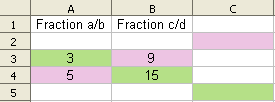
\includegraphics[width=.5\linewidth]{actiTableur}
\end{center}

\item Programme en \texttt{C2} le produit de \texttt{A4} par \texttt{B3} et en \texttt{C5} le produit de \texttt{A3} par \texttt{B4}.
\item Teste dans le tableur les trois fractions trouvées à la question 1. Que remarques-tu dans les cellules \texttt{C2} et \texttt{C5} ?
\item En te servant du tableur, trouve parmi les nombres en écriture fractionnaire suivants ceux qui sont égaux à $\dfrac{3}{5}$ : $\dfrac{301}{501}$ ; $\dfrac{192}{320}$ ; $\dfrac{8,1}{13,5}$ ; $\dfrac{2500}{4000}$.
\item Un nombre en écriture fractionnaire égal à $\dfrac{3}{5}$ s'écrit sous la forme $\dfrac{3\,k}{5\,k}$ où $k$ est un nombre non nul. Démontre que leurs produits en croix sont égaux.
\item On veut déterminer la fraction de dénominateur 120 égale à la fraction $\dfrac{3}{5}$. Remplis les cellules du tableur que l'on connaît et programme en \texttt{B3} le nombre cherché.
\item De la même façon, trouve les nombres manquants : $\dfrac{3}{5}=\dfrac{...}{75}$ ; $\dfrac{3}{5}=\dfrac{...}{125}$ ; $\dfrac{3}{5}=\dfrac{...}{0,25}$.
\end{enumerate}
\end{activite}


%%%%%%%%%%%%%%%%%%%%%%%%%%%%%%%%%%%%%%%%%%%%%%%


\begin{activite}[Inverses]
\begin{enumerate}
\item Quelle est la longueur du côté d'un carré d'aire 1 unité d'aire (U.A.) ?
\item On considère plusieurs rectangles qui ont tous la même aire de 1 U.A.. Recopie puis complète le tableau suivant par les nombres qui conviennent :
 
\renewcommand*\tabularxcolumn[1]{>{\centering\arraybackslash}m{#1}}
\renewcommand{\arraystretch}{1.6}
\begin{CLtableau}{\linewidth}{7}{c}
\hline
& Rectangle 1 & Rectangle 2 & Rectangle 3 & Rectangle 4 & Rectangle 5 & Rectangle 6 \\ \hline
Longueur & 2 & & & 3 & & $\dfrac{4}{3}$ \\ \hline
Largeur & & $0,1$ & $0,25$ & & $\dfrac{1}{7}$ & \\ \hline
\end{CLtableau}

    \begin{enumerate}
        \item Que dire de la longueur de ces rectangles ? Et de la largeur ?
        \item Quel lien y a-t-il entre la longueur et la largeur de ces rectangles ?
        
        \textbf{On dit que deux nombres sont inverses l'un de l'autre quand leur produit est égal à 1.}
        
        \item Recopie et complète : les nombres 2 et ... sont inverses l'un de l'autre, ainsi que $0,1$ et ... ; $0,25$ et ... ; 3 et ... ; $\dfrac{1}{7}$ et ... ; $\dfrac{4}{3}$ et ... .
        
        Que peux-tu dire pour le nombre 1 ?
        
        \item Soit $x$ un nombre non nul, quel est l'inverse de $x$ ? Justifie.
        \item Soient $a$ et $b$ deux nombres non nuls, quel est l'inverse de $\dfrac{a}{b}$ ? Justifie.
    \end{enumerate}
 
\end{enumerate}
\end{activite}



%%%%%%%%%%%%%%%%%%%%%%%%%%%%%%%%%%%%%%%%%%%%%%%



\begin{activite}[Comparaison dans tous les cas]

\begin{partie}[Dénominateurs n'ayant pas de diviseur commun autre que 1]
Corentin le lapin et Luce la puce décident de faire une course. Corentin fait des bonds de $\dfrac{1}{3}$ de mètre tandis que Luce fait des bonds de $\dfrac{1}{5}$ de mètre. 

\begin{center}
    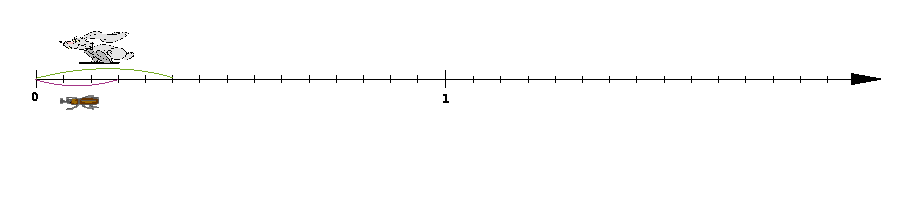
\includegraphics[width=\linewidth]{actiLapinScara}
\end{center}

    \begin{enumerate}
        \item Quand Corentin fait deux bonds, Luce en fait trois. Reproduis la demi-droite graduée ci-dessus représentant la course, puis place les points $C$ et $L$ pour indiquer les positions de Corentin et de Luce.
        \item Complète les phrases suivantes :
        
« Corentin a parcouru $\dfrac{...}{...}$ de mètre, ce qui équivaut à $\dfrac{...}{15}$ de mètre. »

« Luce a parcouru $\dfrac{...}{...}$ de mètre, ce qui équivaut à $\dfrac{...}{15}$ de mètre. »

        \item En t'aidant de la question 2, indique lequel des deux a parcouru la plus grande distance. Parmi les fractions $\dfrac{2}{3}$ et $\dfrac{3}{5}$, laquelle est la plus grande ?
    \end{enumerate}
\end{partie}

\begin{partie}[Dénominateurs ayant plusieurs diviseurs communs]
Lola la tortue et Jeannot le lièvre décident de faire une course sur une demi-droite graduée. Le point de départ est l'origine de la demi-droite. Lola parcourt $\dfrac{5}{4}$ d'unité et Jeannot parcourt $\dfrac{7}{6}$ d'unité.
    \begin{enumerate}
        \item Trace une demi-droite et gradue-la pour y placer les points $L$ et $J$ indiquant les positions de Lola et Jeannot.
        \item Lequel des deux a parcouru le plus grand trajet ? Parmi les fractions $\dfrac{5}{4}$ et $\dfrac{7}{6}$, laquelle est la plus grande ?
    \end{enumerate}
\end{partie}


\begin{partie}[Bilan]
\begin{enumerate}
    \item Énonce une règle qui permet de comparer des fractions de dénominateurs différents.
    \item Applique la règle que tu as trouvée pour comparer : $\dfrac{7}{5}$ et $\dfrac{13}{11}$ puis $\dfrac{3}{25}$ et $\dfrac{1}{10}$.
\end{enumerate}
\end{partie}

\end{activite}

%%%%%%%%%%%%%%%%%%%%%%%%%%%%%%%%%%%%%%%%%%%%%%%


\begin{activite}[Divisions]
\begin{enumerate}
\item Sachant que pour tous nombres $a$ et $b$ non nuls : $\dfrac{a}{b}=a \times \dfrac{1}{b}$, décompose de la même façon le quotient $\dfrac{\dfrac{3}{2}}{\dfrac{5}{3}}$.
\item Que peux-tu dire du nombre $\dfrac{1}{\dfrac{5}{3}}$ ? Déduis-en une fraction égale à ce nombre.
\item Transforme alors le quotient $\dfrac{\dfrac{3}{2}}{\dfrac{5}{3}}$ en produit et complète la phrase suivante : \emph{« Diviser par une fraction, c'est ... .».}
\item Termine alors le calcul du quotient de $\dfrac{3}{2}$ par $\dfrac{5}{3}$.
\item Applique cette règle pour effectuer les calculs suivants : $\dfrac{\dfrac{10}{11}}{\dfrac{7}{8}}$ ; $\dfrac{\dfrac{4}{7}}{\dfrac{5}{9}}$ ; $\dfrac{\dfrac{2}{5}}{\dfrac{14}{3}}$.
\end{enumerate}
\end{activite}


\cours
\section{Amplifier ou réduire un quotient}

\begin{aconnaitre}
\textbf{Si on multiplie ou si on divise} le numérateur et le dénominateur d'un quotient par \textbf{un même nombre non nul} alors on obtient \textbf{quotient égal}.

Pour tous nombres $a$, $b$ et $k$ où $b$ et $k$ sont non nuls :
\[ \frac{a \times k}{b \times k} = \frac{a}{b} \text{ et } \frac{a \div k}{b \div k} = \frac{a}{b}\]
\end{aconnaitre}

\begin{exemple*1}
Simplifie le quotient $\dfrac{42}{-140}$.
\correction

\begin{tabular}{lll}
$\dfrac{42}{-140}=-\dfrac{42}{140}$ & $\longrightarrow$ & On détermine le signe du quotient. \\
$\dfrac{42}{-140}=-\dfrac{3 \times 2 \times 7}{10 \times 7 \times 2}$  & $\longrightarrow$ & On cherche les facteurs communs à 2 et 140. \\
$\dfrac{42}{-140}=-\dfrac{3}{10}$ & $\longrightarrow$ & On simplifie le quotient. \\
\end{tabular}
\end{exemple*1}

\begin{exemple*1}
Détermine le nombre manquant dans l'égalité $\dfrac{-1,2}{6}=\dfrac{...}{18}$.
\correction

\vspace{.5em}
\begin{tabular}{lll}
\hspace{1.5em}
\includegraphics[width=.8cm]{figX3} & & \\
$\dfrac{-1,2}{6}=\dfrac{...}{18}$ & $\longrightarrow$ & Pour passer de 6 à 18 \textbf{on multiplie par 3}. \\
\hspace{1.5em}
\includegraphics[width=.8cm]{figX3b} & & \\
donc $\dfrac{-1,2}{6}=\dfrac{-3,6}{18}$  & $\longrightarrow$ & Ainsi, pour trouver le nombre manquant, \textbf{on multiplie} \\
& & \textbf{$\mathbf{-1,2}$ par 3}, ce qui donne $-3,6$. \\
\end{tabular}
\end{exemple*1}


\section{Comparer deux fractions}

\begin{aconnaitre}[Fractions dont le numérateur et le dénominateur sont positifs]
\begin{itemize}
\item Si les deux fractions ont le même dénominateur, la plus grande est celle qui a le plus grand numérateur.

Par exemple $\dfrac{5}{7}>\dfrac{2}{7}$ car $5 > 2$.

\item Si les deux fractions ont le même numérateur, la plus grande est celle qui a le plus petit dénominateur.

Par exemple $\dfrac{4}{9}<\dfrac{4}{5}$ car $9 > 5$.

\item Si une fraction est plus grande que 1 (son numérateur est plus grand que son dénominateur), alors elle est plus grande qu'une fraction qui est plus petite que 1 (dont le numérateur est plus petit que le dénominateur).

Par exemple $\dfrac{9}{5}>\dfrac{6}{7}$ car $\dfrac{9}{5}>1$ et $\dfrac{6}{7}<1$. 
\end{itemize}
\end{aconnaitre}



\begin{remarque}
Attention, les règles données ci-dessus ne sont pas vraies si le numérateur ou le dénominateur d'une des fractions est négatif.
\end{remarque}

\section{Multiplication}

\begin{aconnaitre}
Pour \textbf{multiplier des nombres en écriture fractionnaire}, on multiplie les numérateurs entre eux et les dénominateurs entre eux.

Pour tous nombres $a$, $b$, $c$ et $d$ où $b$ et $d$ sont non nuls :
\[ \dfrac{a}{b} \times \dfrac{c}{d} = \dfrac{a\times c}{b \times d} \]
\end{aconnaitre}

\begin{remarque}
Si $b=1$, la formule devient $a \times \dfrac{c}{d} = \dfrac{a\times c}{d}$
\end{remarque}

\begin{exemple*1}
Calcule l'expression $B=-\dfrac{35}{33} \times \dfrac{-39}{-80}$. Donne le résultat sous forme simplifiée.
\correction
\vspace{.5em}
 
\begin{tabular}{lll}
$B = -\dfrac{35 \times 39}{33 \times 80}$ & $\longrightarrow$ & On détermine le signe du résultat. \\
$B = -\dfrac{7 \times \mathbf{5} \times 13 \times \mathbf{3}}{11 \times \mathbf{3} \times 2 \times \mathbf{5} \times 8}$ & $\longrightarrow$ & On cherche des facteurs communs. \\
$B = -\dfrac{7 \times 13}{11 \times 2 \times 8}$ & $\longrightarrow$ & On simplifie. \\
$B = -\dfrac{91}{176}$ & $\longrightarrow$ & On calcule. \\
\end{tabular}
\end{exemple*1}

\section{Division de deux quotients}

\subsection{Inversion d'un nombre non nul}

\begin{definition}
\textbf{Deux nombres sont \MotDefinition{inverses}{}} l'un de l'autre si leur produit est égal à 1.
\end{definition}

\begin{propriete}
\begin{itemize}
    \item Tout nombre $x$ non nul admet un inverse qui est le nombre $\dfrac{1}{x}$.
    \item Tout nombre en écriture fractionnaire $\dfrac{a}{b}$ ($a\neq 0$ et $b \neq 0$) admet un inverse qui est le nombre $\dfrac{b}{a}$.
\end{itemize}
\end{propriete}

\begin{remarque}
\begin{itemize}
    \item Un nombre et son inverse ont toujours le même signe.
    
    En effet, leur produit 1 est positif et seul le produit de deux nombres de même signe est positif.
    \item Zéro est le seul nombre qui n'admet pas d'inverse.
    
    En effet, tout nombre multiplié par 0 donne 0 et ne donnera jamais 1.
\end{itemize}
\end{remarque}

\begin{exemple}
Calcule l'inverse de 3.
\correction
L'inverse de 3 est $\dfrac{1}{3}$.
\end{exemple}

\begin{exemple}
Calcule l'inverse de $\dfrac{-7}{3}$.
\correction
L'inverse de $\dfrac{-7}{3}$ est $\dfrac{1}{\dfrac{-7}{3}}=\dfrac{3}{-7}=\dfrac{-3}{7}$.
\end{exemple}

\subsection{Diviser des quotients}

\begin{aconnaitre}
\textbf{Diviser par un nombre non nul} revient à multiplier par l'inverse de ce nombre.

Pour tous nombres $a$, $b$, $c$ et $d$ où $b$, $c$ et $d$ sont non nuls :
\[ \dfrac{a}{b} \div \dfrac{c}{d} = \dfrac{a}{b} \times \dfrac{d}{c} \text{ ou } \dfrac{\phantom{i}\dfrac{a}{b}\phantom{i}}{\dfrac{c}{d}}=\dfrac{a}{b} \times \dfrac{d}{c} \]
\end{aconnaitre}

\begin{exemple*1}
Calcule $C=\dfrac{-8}{7} \div \dfrac{5}{-3}$.
\correction
\vspace{.5em}
 
\begin{tabular}{lll}
$C=+\left(\dfrac{8}{7} \div \dfrac{5}{3}\right)$ & $\longrightarrow$ & On détermine le signe du résultat. \\
$C=\dfrac{8}{7} \times \dfrac{3}{5}$ & $\longrightarrow$ & On multiplie par l'inverse du deuxième quotient. \\
$C=\dfrac{8\times 3}{7\times 5}$ & $\longrightarrow$ & On multiplie les fractions. \\
$C=\dfrac{24}{35}$ & $\longrightarrow$ & On calcule. \\
\end{tabular}
\end{exemple*1}


\begin{exemple*1}
Calcule $D=\dfrac{-\dfrac{32}{21}}{\dfrac{-48}{-35}}$ et donne le résultat en le simplifiant le plus possible.
\correction
\vspace{.5em}
 
\begin{tabular}{lll}
$D=-\dfrac{\dfrac{32}{21}}{\dfrac{48}{35}}$ & $\longrightarrow$ & On détermine le signe du résultat. \\
$D=-\dfrac{32}{21}\times \dfrac{35}{48}$ & $\longrightarrow$ & On multiplie par l'inverse du deuxième quotient. \\
$D=-\dfrac{\mathbf{8}\times \mathbf{2}\times 2 \times \mathbf{7} \times 5}{\mathbf{7 \times 3 \times 3 \times \mathbf{2} \times \mathbf{8}}}$ & $\longrightarrow$ & On cherche des facteurs communs. \\
$D=-\dfrac{10}{9}$ & $\longrightarrow$ & On calcule sans oublier de simplifier avant ! \\
\end{tabular}
\end{exemple*1}


\begin{exemple*1}
Quelle est la nature du nombre $E$ défini par $E=\dfrac{1+\dfrac{2}{3}}{1-\dfrac{2}{3}}$ ?
\correction
\vspace{.5em}
 
\begin{tabular}{lll}
$E=\dfrac{\dfrac{3}{3}+\dfrac{2}{3}}{\dfrac{3}{3}-\dfrac{2}{3}}=\dfrac{\dfrac{5}{3}}{\dfrac{1}{3}}$ & $\longrightarrow$ & $E$ peut s'écrire aussi $E=\left(1+\dfrac{2}{3}\right) \div \left(1-\dfrac{2}{3}\right)$. \\
 & & On commence donc par calculer les parenthèses.\\
$E=\dfrac{5}{3} \times \dfrac{3}{1}$ & $\longrightarrow$ & On multiplie par l'inverse du deuxième quotient. \\
$E=\dfrac{5\times \mathbf{3}}{\mathbf{3}\times 1}$ & $\longrightarrow$ & On cherche des facteurs communs. \\
$E=5$ donc $E$ est un nombre entier. & &  \\
\end{tabular}
\end{exemple*1}


\section{Signe d'une fraction}

\begin{propriete}
Pour déterminer le signe d'une fraction, on utilise la règle du produit des signes.
\end{propriete}

\begin{aconnaitre}
Si une fraction est négative, on peut l'écrire de trois manières différentes en mettant le signe moins au numérateur, au dénominateur (peu utilisé) ou devant la fraction.
On écrira donc indifféremment  $\dfrac{-2}{3}$ ou $-\dfrac{2}{3}$ et rarement $\dfrac{2}{-3}$.
\end{aconnaitre}



\exercicesbase
\begin{colonne*exercice}
\serie{Comparaison}


\begin{exercice}[Signes]
Donne le signe des nombres suivants :

$\dfrac{-5,2}{4,23}$ ; $\dfrac{5}{-2,1}$ ; $\dfrac{472}{23}$ ; $\dfrac{-8,9}{-45}$ ; $-\dfrac{12}{13}$ ; $-\dfrac{11}{-5,2}$.
\end{exercice}





\begin{exercice}
Indique les nombres égaux parmi ceux de la liste ci-dessous :

$\dfrac{-8}{9}$ ; $-\dfrac{8}{9}$ ; $\dfrac{-8}{-9}$ ; $-\dfrac{8}{-9}$ ; $\dfrac{8}{-9}$ ; $-\dfrac{-8}{9}$ ; $\dfrac{8}{9}$.
\end{exercice}




\begin{exercice}[Encadrement]

\begin{enumerate}
\item On considère la fraction $\dfrac{56}{21}$.

Effectue la division euclidienne de 56 par 21 et déduis-en un encadrement de la fraction par deux nombres entiers consécutifs.
\item Encadre $\dfrac{-89}{15}$ puis $\dfrac{47}{59}$ par deux nombres entiers consécutifs.
\item Encadre respectivement $\dfrac{-47}{25}$ et $\dfrac{13}{-4}$ par deux nombres entiers consécutifs et déduis-en la comparaison de ces deux fractions.
\item Peux-tu appliquer la même méthode pour comparer $\dfrac{25}{3}$ et $\dfrac{90}{11}$ ?
\end{enumerate}
\end{exercice}




\begin{exercice}[Avec des valeurs approchées]
Soient deux nombres : $a =\dfrac{816}{577}$  et $b =\dfrac{577}{408}$.
\begin{enumerate}
\item Donne la valeur arrondie de $a$ et celle de $b$ au millième. Peux-tu en déduire la comparaison de $a$ et de $b$ ?
\item Donne des valeurs approchées de $a$ et $b$ qui permettent de les comparer. Compare $a$ et $b$.
\end{enumerate}
\end{exercice}





\begin{exercice}[Égalités]
Recopie et complète chacune des égalités suivantes :
\begin{enumerate}
\item $\dfrac{...}{-5}=\dfrac{10}{20}$
\item $\dfrac{2}{3}=\dfrac{...}{27}$
\item $\dfrac{-15}{45}=\dfrac{-5}{...}$
\item $\dfrac{...}{-18}=\dfrac{7}{6}$
\item $3=\dfrac{...}{4}$
\item $-2,1=-\dfrac{21}{...}$
\end{enumerate}
\end{exercice}




\begin{exercice}
Dans chaque cas, à partir des égalités données et en utilisant seulement les quatre nombres qui apparaissent, écris toutes les égalités d'écritures fractionnaires possibles :
\begin{enumerate}
\item $7 \times (-8) = -4 \times 14$
\item $-3 \times (-1) = 2 \times 1,5$
\item $2,1 \times 12 = 9 \times 2,8$
\item $-4 \times 9 = 12 \times (-3)$
\end{enumerate}
\end{exercice}




\begin{exercice}[Égalité ?]
Recopie et complète en utilisant $=$ ou $\neq$, en justifiant dans chaque cas :
\begin{enumerate}
\item $\dfrac{9}{5} ... \dfrac{26}{15}$ 
\item $\dfrac{-7}{-3} ... \dfrac{-14}{6}$
\item $\dfrac{-12,7}{-5} ... \dfrac{25,4}{10}$
\item $\dfrac{-27,35}{27,35} ... \dfrac{15,72}{-15,72}$
\end{enumerate}
\end{exercice}





\begin{exercice}[Avec un dénominateur entier positif]
Réécris chacune des écritures fractionnaires suivantes avec un dénominateur entier positif :
$\dfrac{4}{-5}$ ; $\dfrac{-8}{-7}$ ; $-\dfrac{5,2}{-7}$ ; $\dfrac{7}{-2,1}$ ; $\dfrac{8,2}{0,12}$ ; $-\dfrac{-1}{-3,54}$.
\end{exercice}





\begin{exercice}[Même dénominateur positif]
\begin{enumerate}
\item Recopie et complète la phrase suivante :

« Deux nombres en écriture fractionnaire de même dénominateur positif sont rangés... ».
\item Compare les nombres suivants :

$\dfrac{-7,5}{3}$ et $\dfrac{-7,49}{3}$ ;

$\dfrac{4,05}{2,1}$ et $\dfrac{4,2}{2,1}$ ;

$-\dfrac{0,74}{5}$ et $\dfrac{-0,7309}{5}$ ; 

$\dfrac{8}{-5,23}$ et $\dfrac{-7,9}{5,23}$. 
\end{enumerate}
\end{exercice}





\begin{exercice}[Avec le même numérateur]
\begin{enumerate}
\item Recopie et complète la phrase suivante :

« Deux nombres positifs en écriture fractionnaire de même numérateur sont rangés… »
\item Compare les nombres suivants :

$\dfrac{3,5}{8,2}$ et $\dfrac{3,5}{8,15}$ ;

$-\dfrac{-1}{6}$ et $\dfrac{1}{5,7}$.
\end{enumerate}
\end{exercice}




\begin{exercice}[Avec le même numérateur (bis)]
Compare les nombres suivants en commençant par comparer leurs opposés :
\begin{enumerate}
\item $\dfrac{1}{-5}$ et $\dfrac{1}{-7}$ ;
\item $\dfrac{-3}{8}$ et $\dfrac{-3}{8,2}$ ;
\item $-\dfrac{5,23}{14,5}$ et $\dfrac{-5,23}{14,6}$ ;
\item $\dfrac{-7,5}{0,23}$ et $\dfrac{75}{-2,4}$. 
\end{enumerate}
\end{exercice}





\begin{exercice}
Dans chaque cas, réécris les nombres avec le même dénominateur positif puis compare-les :
\begin{enumerate} 
\item $\dfrac{-5}{4}$ et $\dfrac{-9}{8}$ ;
\item $\dfrac{2,7}{-9}$ et $\dfrac{-1}{3}$ ;
\item -3 et $-\dfrac{20,9}{-7}$ ;
\item $-\dfrac{2}{11}$ et $\dfrac{-5}{33}$ ; 
\item $\dfrac{7}{2,5}$ et $\dfrac{-20,5}{7,5}$ ; 
\item $\dfrac{13}{-27}$ et $\dfrac{-79}{162}$.
\end{enumerate}
\end{exercice}




\begin{exercice}[Multiple commun]
\begin{enumerate}
\item Quels sont les dix premiers multiples de 12 ? Ceux de 18 ? Déduis-en le plus petit multiple non nul commun à 12 et 18, puis un dénominateur commun positif des fractions : $\dfrac{-7}{12}$ et $\dfrac{-11}{18}$.

Compare alors ces deux nombres.
\item La méthode précédente permet-elle de trouver rapidement un dénominateur commun aux nombres : $\dfrac{8}{11}$ et $\dfrac{10}{13}$ ?

Comment en trouver un alors rapidement ? Compare ces deux nombres.
\end{enumerate}
\end{exercice}





\begin{exercice}Dans chaque cas, réécris les nombres avec le même dénominateur positif, puis compare-les :
\begin{enumerate}
\item $\dfrac{-5}{8}$ et $\dfrac{-3,8}{6}$ ;
\item $\dfrac{14}{5}$ et $\dfrac{20}{7}$ ;
\item $\dfrac{3}{-50}$ et $-\dfrac{4}{75}$ ;
\item $\dfrac{54,5}{0,27}$ et $\dfrac{-2,62}{0,13}$.
\end{enumerate}
\end{exercice}






\begin{exercice}
Compare en justifiant :
\begin{enumerate}
\item $-\dfrac{12}{18}$ et $\dfrac{399}{-300}$ ; 
\item $\dfrac{2}{57}$ et $\dfrac{1}{28,4}$ ;
\item $\dfrac{-75}{47}$ et $\dfrac{25}{-15}$ ;
\item $\dfrac{-5}{6}$ et $-\dfrac{15}{14}$ ;
\item $\dfrac{6}{13}$ et $\dfrac{29}{65}$ ;
\item $\dfrac{3}{-22}$ et $\dfrac{4,5}{33}$.
\end{enumerate}
\end{exercice}




\begin{exercice}[Dans l'ordre]
\begin{enumerate}
\item Range les nombres suivants dans l'ordre croissant sans utiliser de valeurs approchées :

$\dfrac{7}{-15}$ ; $\dfrac{7}{3}$ ; $\dfrac{490}{420}$ ; $\dfrac{-5}{12}$ ; $\dfrac{-24}{-18}$ ; 2,5.
\item Range les nombres suivants dans l'ordre décroissant :

$\dfrac{-29}{100}$ ; $\dfrac{7}{-25}$ ; $-0,285$ ; $-\dfrac{1}{5}$ ; $\dfrac{13}{-50}$ ; 0 ; $\dfrac{-1}{2,5}$.
\end{enumerate}
\end{exercice}





\begin{exercice}[Trajet]
Quatre amis font un voyage en trois jours. Le premier jour, ils parcourent 40\,\%\ du trajet total ; le deuxième jour, un quart et le dernier jour, $\dfrac{7}{20}$ du trajet total.

Quel jour ont-ils parcouru la plus grande distance ?

Peux-tu calculer la distance parcourue chaque jour ?
\end{exercice}







\serie{Multiplications}





\begin{exercice}[La règle et les signes]
Effectue les produits suivants :
\begin{enumerate}
\item $\dfrac{3}{2} \times \dfrac{5}{7}$ ;
\item $\dfrac{-4}{11} \times \dfrac{1}{-3}$ ;
\item $3 \times \dfrac{-7}{5}$ ;
\item $\dfrac{5}{-4} \times \dfrac{5}{-2}$ ;
\item $\dfrac{8}{17} \times \dfrac{5}{-3}$ ;
\item $-\dfrac{13}{5} \times \left(-\dfrac{2}{11}\right)$ ;
\item $\left(-\dfrac{7}{15}\right) \times (-8) \times \dfrac{2}{3}$ ;
\item $\dfrac{-1}{2} \times \dfrac{5}{-4} \times \dfrac{-3}{2}$.
\end{enumerate}
\end{exercice}





\begin{exercice}[Toujours plus simple]
Simplifie, si possible, les écritures fractionnaires suivantes :
\begin{enumerate}
\item $\dfrac{-5 \times 2}{2 \times 7}$ ;  
\item $\dfrac{-5 + 2}{7 + 2}$ ;
\item $\dfrac{4 \times (-11)}{4 \times (-11) \times 3}$ ;
\item $\dfrac{8 \times (-3) \times 7 \times 5}{3 \times 5 \times 8 \times 7}$ ;
\item $\dfrac{-5 \times 8}{2 \times (-7)}$ ;
\item $\dfrac{5 \times (-9) \times 2}{(-7) \times 10 \times (-1)}$ ;
\end{enumerate}
\end{exercice}





\begin{exercice}[Calculer en simplifiant]
Pour chacun des produits suivants, applique la règle de multiplication sans effectuer les calculs, simplifie lorsque cela est possible et donne alors le résultat sous la forme d'une fraction irréductible :
\begin{enumerate}
\item $\dfrac{8}{5} \times \dfrac{5}{7}$ ;
\item $\dfrac{-3}{10} \times \dfrac{-11}{3}$ ;
\item $\dfrac{-2}{3} \times \dfrac{-5}{2} \times \dfrac{3}{-7}$ ;
\item $\dfrac{5}{-7} \times \left(-\dfrac{7}{5}\right)$ ;
\item $-15 \times \dfrac{2}{15}$ ;
\item $\left(-\dfrac{8}{3}\right) \times \left(-\dfrac{1}{5}\right) \times 3$.
\end{enumerate}
\end{exercice}




\begin{exercice}Complète les égalités  suivantes :
\begin{enumerate}
\item $\dfrac{8}{...} \times \dfrac{7}{3} = -\dfrac{8}{3}$ ; 
\item $\dfrac{-5}{3} \times \dfrac{7}{...} = \dfrac{7}{6}$ ;
\item $\dfrac{6}{5} \times ... = -6$ ;
\item $\left(-\dfrac{8}{21}\right) \times \dfrac{...}{...} = 1$ ;
\item $\dfrac{...}{10} \times \dfrac{7}{...} = -5$ ;
\item $\dfrac{...}{-9} \times \dfrac{2}{...} = \dfrac{4}{15}$ ;
\item $\dfrac{-5}{...} \times \dfrac{3}{-14} \times \dfrac{...}{25} = \dfrac{-2}{7}$.
\end{enumerate}
\end{exercice}




\begin{exercice}[Simplifier avant de calculer]
\begin{enumerate}
\item Écris 15 sous la forme d'un produit de deux nombres entiers. Décompose de même 20 en produit de nombres entiers positifs les plus petits possibles.
\item Recopie et complète les égalités suivantes :
$\dfrac{15}{7} \times \dfrac{11}{20} = \dfrac{... \times ...}{... \times ...} = \dfrac{(... \times ...) \times ...}{... \times (... \times ... \times ...)}$.
\item Simplifie l'expression obtenue et donne le résultat sous forme d'une fraction irréductible.
\end{enumerate}
\end{exercice}





\begin{exercice}
Calcule les produits suivants en simplifiant, puis donne les résultats sous la forme d'une fraction irréductible :
\begin{enumerate}
\item $\dfrac{-7}{25} \times \dfrac{-5}{8}$ ;
\item $\dfrac{18}{-49} \times \dfrac{14}{27}$ ;
\item $\dfrac{45}{28} \times \dfrac{7}{-15}$ ;
\item $\dfrac{-2}{6} \times \left(-\dfrac{21}{11}\right)$ ;
\item $\dfrac{21}{32} \times \dfrac{108}{49}$ ;
\item $-26 \times \dfrac{-5}{39}$ ;
\item $\dfrac{8}{5} \times \dfrac{-5}{21} \times \left(-\dfrac{9}{16}\right)$ ;
\item $\dfrac{56}{-5} \times \dfrac{30}{21} \dfrac{7}{10}$.
\end{enumerate}
\end{exercice} 




\begin{exercice}[Avec la calculatrice]
Utilise ta calculatrice pour effectuer les produits suivants et donne les résultats sous la forme d'une fraction irréductible :
\begin{enumerate}
\item $\dfrac{686}{-153} \times \dfrac{-99}{-196}$ ; 
\item $\dfrac{2,1}{12,5} \times \left(-\dfrac{6,25}{0,49}\right)$.
\end{enumerate}
\end{exercice}



\begin{exercice}
Calcule mentalement :
\begin{enumerate}
\item les trois quarts de 400 ;
\item le double de $\dfrac{-7}{15}$ ;
\item les cinq septièmes des six cinquièmes de l'unité ;
\item les $\dfrac{7}{10}$ de $\dfrac{9}{10}$.
\end{enumerate}
\end{exercice}




\begin{exercice}[Dépense]
Abdel dépense les $\dfrac{5}{12}$ de son argent de poche, puis les trois quarts de ce qu'il lui reste alors.
\begin{enumerate}
\item Quelle fraction de son argent de poche a-t-il dépensée la deuxième fois ?
\item Le montant de son argent de poche étant de 72\,€, combien a-t-il dépensé au total ?
\end{enumerate}
\end{exercice}



\begin{exercice}
Recopie et complète en utilisant $=$ ou $\neq$, en justifiant dans chaque cas :
\begin{enumerate}
\item $\dfrac{-9,1}{5,2} ... \dfrac{79,8}{-45,6}$ ;
\item $\dfrac{-5}{-3} ... \dfrac{-3,5}{2,1}$ ;
\item $\dfrac{17,36}{-22,32} ... -\dfrac{28,7}{36,9}$ ;
\item $\dfrac{-56}{-57} ... \dfrac{57}{58}$ ;
\end{enumerate}
\end{exercice}





\serie{Divisions}


\begin{exercice}Inverses
Recopie et complète les égalités suivantes et écris, dans chaque cas, trois phrases utilisant le mot « inverse(s) » :
\begin{enumerate}
\item $4 \times \dfrac{1}{...} = 1$ ;
\item $... \times 0,25 = 1$ ;
\item $\dfrac{1}{...} \times (-3) = 1$ ;
\item $... \times \left(-\dfrac{1}{15}\right) = 1$ ;
\item $\dfrac{3}{4} \times \dfrac{...}{...} = 1$ ;
\item $\dfrac{...}{-25} \times \dfrac{...}{7} = 1$ ;
\item $... \times \left(-\dfrac{8}{5}\right) = 1$ ;
\item $-0,01 \times ... = 1$
\end{enumerate}
\end{exercice}



\begin{exercice}[Ne pas confondre !]
\begin{enumerate}
\item Recopie et complète les égalités suivantes :
\[ \left(\dfrac{9}{-14}\right) \times ... = 1 et \left(\dfrac{9}{-14}\right) + ... = 0\].
Écris deux phrases, l'une utilisant le mot « opposé(s) » et l'autre, le mot « inverse(s) ».
\item Trouve deux nombres qui sont leur propre inverse. Trouve un nombre qui est son propre opposé.
\item Tous les nombres ont-ils un inverse ? Un opposé ?
\item Quel est l'opposé de l'inverse de 4 ? Quel est l'inverse de l'opposé de 4 ?
\end{enumerate}
\end{exercice}



\begin{exercice}[Inverse]
\begin{enumerate}
\item Recopie et complète le tableau ci-dessous avec des écritures fractionnaires.

\renewcommand*\tabularxcolumn[1]{>{\centering\arraybackslash}m{#1}}
\renewcommand{\arraystretch}{1.6}
\begin{Ctableau}{\linewidth}{7}{c}
\hline
$x$ & 7 & $\dfrac{-3}{5}$ & $-\dfrac{8}{9}$ & $-0,6$ & $1,25$ \\ \hline
$\dfrac{1}{x}$ & & & & & \\ \hline
\end{Ctableau}
\item Détermine l'inverse de l'inverse de chaque nombre. Que remarques-tu ?
\end{enumerate}
\end{exercice}


\begin{exercice}[Mentalement]
\begin{enumerate}
\item Effectue mentalement les calculs suivants : $16 \div 2$ ; $100 \times 0,25$ ; $16 \times 0,5$ ; $100 \div 4$.
\item Justifie les résultats égaux avec la règle de division.
\end{enumerate}
\end{exercice}


\begin{exercice}La règle
Applique dans chaque cas la règle de division puis effectue les calculs :
\begin{enumerate}
\item $\dfrac{2}{3} \div 5$ ; 
\item $\dfrac{-5}{7} \div (-4)$ ;
\item $\dfrac{5}{6} \div \dfrac{7}{-11}$ ;
\item $8 \div \dfrac{1}{8}$ ;
\item $\dfrac{-3}{2} \div \dfrac{-5}{7}$ ;
\item $\dfrac{1}{10} \div \left(-\dfrac{7}{9}\right)$.
\end{enumerate}
\end{exercice}

\begin{exercice}Trait de fraction
Écris les quotients suivants en utilisant le symbole $\div$ puis effectue le calcul :
\[ A = \dfrac{2}{\dfrac{3}{5}}  ; B = \dfrac{\dfrac{2}{3}}{5} ; C = \dfrac{\dfrac{2}{3}}{\dfrac{7}{11}}.\]
\end{exercice}


\begin{exercice}[Division et simplification]
Applique la règle de division, simplifie puis effectue les calculs et donne les résultats sous la forme d'une fraction irréductible :
\begin{enumerate}
\item $\dfrac{8}{-15} \div \dfrac{-4}{5}$ ;
\item $\dfrac{9}{10} \div (-3)$ ;
\item $\dfrac{-4}{45} \div \dfrac{16}{15}$ ;
\item $\dfrac{-5}{6} \div \left(-\dfrac{15}{18}\right)$ ;
\item $12 \div \dfrac{3}{-4}$ ;
\item $1 \div \left(\dfrac{-7}{4}\right)$.
\end{enumerate}
\end{exercice}

\end{colonne*exercice}


\exercicesappr
\begin{colonne*exercice}
%\begin{exercice}[Partage]
\begin{enumerate}
\item Calcule la moitié de $\dfrac{-5}{12}$.
\item Il reste les $\dfrac{7}{8}$ d'un gâteau.

Trois amis décident de se partager équitablement ce reste : quelle fraction du gâteau aura chacun d'entre eux ?
\end{enumerate}
\end{exercice}


\begin{exercice}[Avec des lettres]
\begin{enumerate}
\item Sachant que $a = \dfrac{-2}{21}$  et $b =\dfrac{5}{-7}$, calcule :
\[	\dfrac{a}{b} ; \dfrac{b}{a} ; a \times b ; a + b \text{ et } a - b\]
Tu donneras les résultats sous la forme d'une fraction irréductible.
\item Même consigne avec $a =\dfrac{5}{24}$  et $b =-\dfrac{35}{18}$.
\end{enumerate}
\end{exercice}


\begin{exercice}
Jenny avait 145 fr. Elle a dépensé les $\dfrac{2}{5}$ de ce qu'elle avait. Combien d’argent lui reste-t-il ?
\end{exercice}


\begin{exercice}
Un salarié gagne 3900 CHF par mois. Il dépense $\dfrac{3}{20}$ de cette somme pour son loyer, $\dfrac{1}{13}$ pour les impôts et 2000 CHF pour vivre. Combien économise-t-il chaque mois ?
\end{exercice}

\columnbreak
\begin{exercice}
J'ai dépensé les $\dfrac{4}{5}$ de mon argent pour acheter un livre qui coûtait 32 CHF. Quelle somme avais-je dans mon porte-monnaie?
\end{exercice}


\begin{exercice}
Olivier a les $\dfrac{7}{16}$ des $\dfrac{2}{3}$ de l'âge de sa mère qui a 48 ans. Quel est l’âge d’Olivier ?
\end{exercice}


\begin{exercice}
Pierre dit à sa sœur pour l'impressionner: « Ce livre a coûté très cher. Je l'ai payé $\dfrac{5}{12}$ des $\dfrac{6}{5}$ de 20 CHF. » Quel est le prix du livre ?
\end{exercice}


\begin{exercice}
Alicia et Alizée ont groupé leurs économies pour s’acheter un lecteur MP3 et des DVD. 

Elles ont dépensé les $\dfrac{6}{10}$ de leur pactole pour l'achat du lecteur MP3 et les $\dfrac{6}{9}$ de ce qu'il restait pour l’acquisition des DVD. Après ces achats, il ne leur reste plus que 28 €.
\begin{enumerate}
\item De quelle somme disposaient-elles avant de faire leurs achats ? 
\item Quel est le prix du lecteur MP3 et celui des DVD ?
\end{enumerate}
\end{exercice}


\begin{exercice}
Monsieur Reesh avait 500 000 CHF dans son coffre mais Arsène Lupin est passé par là et lui a dérobé $\dfrac{3}{4}$ des $\dfrac{5}{6}$ des $\dfrac{4}{5}$ de la somme. Combien lui reste-t-il dans son coffre ?
\end{exercice}


\begin{exercice}
Lors de ses dernières vacances, Alex a dépensé les $\dfrac{3}{4}$ des $\dfrac{5}{9}$ des $\dfrac{7}{10}$ de son argent de poche qui se montait à 3000 CHF. Quelle somme lui reste-t-il ?
\end{exercice}


\end{colonne*exercice}

\connaissances
%\QCMautoevaluation{Pour chaque question, plusieurs réponses sont proposées. Déterminer celles qui sont correctes.}

\begin{QCM}
\begin{GroupeQCM}

\begin{exercice}
La valeur arrondie au dixième de $\dfrac{2}{3}$ est...
\begin{ChoixQCM}{4}
\item $0$
\item $1$
\item $0,6$
\item $0,7$
\end{ChoixQCM}
\begin{corrige}
\reponseQCM{a}
\end{corrige}
\end{exercice}

\begin{exercice}
Une valeur approchée de $\dfrac{19}{13}$ au millième près est...
\begin{ChoixQCM}{4}
\item $1,46$
\item $1,461$
\item $1,462$
\item $1,4615$
\end{ChoixQCM}
\begin{corrige}
\reponseQCM{a}
\end{corrige}
\end{exercice}


\begin{exercice}
$\dfrac{-24}{-18}=...$
\begin{ChoixQCM}{4}
\item $\dfrac{20}{15}$
\item $-\dfrac{4}{3}$
\item $1,33$
\item $\dfrac{4}{3}$
\end{ChoixQCM}
\begin{corrige}
\reponseQCM{a}
\end{corrige}
\end{exercice}


\begin{exercice}
L'opposé de $\dfrac{4}{5}$ est...
\begin{ChoixQCM}{4}
\item $\dfrac{5}{4}$
\item $\dfrac{-4}{-5}$
\item $\dfrac{-4}{5}$
\item $-\dfrac{4}{5}$
\end{ChoixQCM}
\begin{corrige}
\reponseQCM{a}
\end{corrige}
\end{exercice}


\begin{exercice}
$\left(\dfrac{4}{5}\right)^{-1} = ...$
\begin{ChoixQCM}{4}
\item $\dfrac{3}{5}$
\item $\dfrac{-4}{-5}$
\item $\dfrac{5}{4}$
\item $-\dfrac{4}{5}$
\end{ChoixQCM}
\begin{corrige}
\reponseQCM{a}
\end{corrige}
\end{exercice}


\end{GroupeQCM}


\begin{GroupeQCM}

\begin{exercice}
$\dfrac{37}{15}$ est supérieur à...
\begin{ChoixQCM}{4}
\item $2$
\item $\dfrac{77}{30}$
\item $\dfrac{598}{599}$
\item $\dfrac{25}{10}$
\end{ChoixQCM}
\begin{corrige}
\reponseQCM{a}
\end{corrige}
\end{exercice}


\begin{exercice}
$\dfrac{-14}{5}$ est inférieur à...
\begin{ChoixQCM}{4}
\item $\dfrac{14}{-5}$
\item $-2$
\item $\dfrac{-14}{3}$
\item son inverse
\end{ChoixQCM}
\begin{corrige}
\reponseQCM{a}
\end{corrige}
\end{exercice}


\begin{exercice}
$\dfrac{-5}{6}$ est le résultat de...
\begin{ChoixQCM}{4}
\item $\dfrac{-1}{3} \times \dfrac{-5}{2}$
\item $\dfrac{-5}{11} \times \dfrac{11}{6}$
\item $\dfrac{-30}{36} \div 6$
\item $-5 \times \dfrac{1}{6}$
\end{ChoixQCM}
\begin{corrige}
\reponseQCM{a}
\end{corrige}
\end{exercice}


\begin{exercice}
$-\dfrac{7}{5} \div \dfrac{2}{-3}=...$
\begin{ChoixQCM}{4}
\item $2,1$
\item $\dfrac{10}{21}$
\item $\dfrac{3,5}{1,6}$
\item $-\dfrac{21}{10}$
\end{ChoixQCM}
\begin{corrige}
\reponseQCM{a}
\end{corrige}
\end{exercice}


\begin{exercice}
$\dfrac{\dfrac{2}{3}}{4}=...$
\begin{ChoixQCM}{4}
\item $2 \div 3 \div 4$
\item $\dfrac{8}{3}$
\item $\dfrac{2}{12}$
\item On ne peut pas calculer
\end{ChoixQCM}
\begin{corrige}
\reponseQCM{a}
\end{corrige}
\end{exercice}

\end{GroupeQCM}
\end{QCM}

\TravauxPratiques
%\begin{TP}[Dominos en fractions]


Vous allez créer un jeu de dominos utilisant des fractions.

\begin{enumerate}
    \item Répartissez-vous le travail pour compléter le tableau ci-dessous. La première ligne (cases A1 à F1) contient les résultats des calculs situés dans les lignes 2 à 7.

\vspace{1em}
\renewcommand*\tabularxcolumn[1]{>{\centering\arraybackslash}m{#1}}
\renewcommand{\arraystretch}{1.6}
\begin{cltableau}{\linewidth}{7}
\hline
 & A & B & C & D & E & F \\ \hline
1 & $\dfrac{5}{3}$ & $\dfrac{-3}{5}$ & $\dfrac{3}{5}$ & $\dfrac{-9}{4}$ & $\dfrac{2}{7}$ & $3$ \\ \hline
2 & $\dfrac{1}{3} + \dfrac{4}{3}$ & $\dfrac{-4}{5} +\dfrac{1}{5}$ & & & & \\ \hline
3 & $\dfrac{7}{3}-\dfrac{4}{6}$ & $\dfrac{2}{15}-\dfrac{1}{5}-\dfrac{8}{15}$ & & & & \\ \hline
4 & $\dfrac{2}{3}+1$ & $\dfrac{12}{5}-3$ & & & & \\ \hline
5 & & & & & & \\ \hline
6 & & & & & & \\ \hline
7 & & & & & & \\ \hline
\end{cltableau}

\vspace{1em}

Quelques exemples (cases A2, B2, A3, B3, A4, B4) ont été donnés à titre indicatif. Pour chaque colonne, il faut trouver :
\begin{itemize}
    \item ligne 2 : une somme algébrique de fractions de même dénominateur ;
    \item ligne 3 : une somme algébrique de fractions de dénominateurs différents ;
    \item ligne 4 : une somme algébrique d'un nombre entier et d'une fraction ;
    \item ligne 5 : un produit de deux fractions ;
    \item ligne 6 : un produit de trois fractions ;
    \item ligne 7 : un quotient de deux fractions.
\end{itemize}

    \item Créez le jeu de dominos en respectant le plan suivant (à chaque fois, il faut remplacer le nom de la case par son contenu).
    
    Taille d'un domino : 6\,cm sur 2\,cm.
    
    \vspace{1em}
    \begin{center}
        \renewcommand*\tabularxcolumn[1]{>{\centering\arraybackslash}m{#1}}
        \begin{tabularx}{.6\linewidth}{|X|X|X|X|X|X|X|X|}
        \cline{1-2} \cline{4-5} \cline{7-8}
            A1 & A2 & & A3 & B1 & & A4 & C2 \\ \cline{1-2} \cline{4-5} \cline{7-8}
        \end{tabularx}
        \vspace{.5em}
        
        \begin{tabularx}{.6\linewidth}{|X|X|X|X|X|X|X|X|}
        \cline{1-2} \cline{4-5} \cline{7-8}
            A5 & D3 & & A6 & E4 & & A7 & F5 \\ \cline{1-2} \cline{4-5} \cline{7-8}
        \end{tabularx}
        \vspace{.5em}
        
        \begin{tabularx}{.6\linewidth}{|X|X|X|X|X|X|X|X|}
        \cline{1-2} \cline{4-5} \cline{7-8}
            B2 & B3 & & B4 & C1 & & B5 & D2 \\ \cline{1-2} \cline{4-5} \cline{7-8}
        \end{tabularx}
        \vspace{.5em}
        
        \begin{tabularx}{.6\linewidth}{|X|X|X|X|X|X|X|X|}
        \cline{1-2} \cline{4-5} \cline{7-8}
            B6 & E3 & & B7 & F4 & & C3 & C4 \\ \cline{1-2} \cline{4-5} \cline{7-8}
        \end{tabularx}
        \vspace{.5em}
        
        \begin{tabularx}{.6\linewidth}{|X|X|X|X|X|X|X|X|}
        \cline{1-2} \cline{4-5} \cline{7-8}
            C5 & D1 & & C6 & E2 & & C7 & F3 \\ \cline{1-2} \cline{4-5} \cline{7-8}
        \end{tabularx}
        \vspace{.5em}
        
        \begin{tabularx}{.6\linewidth}{|X|X|X|X|X|X|X|X|}
        \cline{1-2} \cline{4-5} \cline{7-8}
            D4 & D5 & & D6 & E1 & & D7 & F2 \\ \cline{1-2} \cline{4-5} \cline{7-8}
        \end{tabularx}
        \vspace{.5em}
        
        \begin{tabularx}{.6\linewidth}{|X|X|X|X|X|X|X|X|}
        \cline{1-2} \cline{4-5} \cline{7-8}
            E5 & E6 & & E7 & F1 & & F6 & F7 \\ \cline{1-2} \cline{4-5} \cline{7-8}
        \end{tabularx}
    \end{center}
    
    \item Découpez les dominos et échangez votre jeu avec un autre groupe. Il ne vous reste plus qu'à jouer en accolant deux cases de même valeur.
\end{enumerate}
\end{TP}

\begin{TP}[Fractions en tableur]

\begin{enumerate}
    \item Calculez puis donnez le résultat sous forme d'une fraction la plus simple possible :
    \[ A = \dfrac{-3}{7} \times \dfrac{5}{2} ; \qquad	B = \dfrac{2}{3} \times \dfrac{9}{2} \]
    \[ C = \dfrac{2}{3} + \dfrac{3}{4} ; \qquad    D = \dfrac{5}{6} + \dfrac{3}{8} \]
    \item Vous allez créer un modèle de fichier tableur permettant de trouver le produit de deux fractions :
    
    \begin{center}
        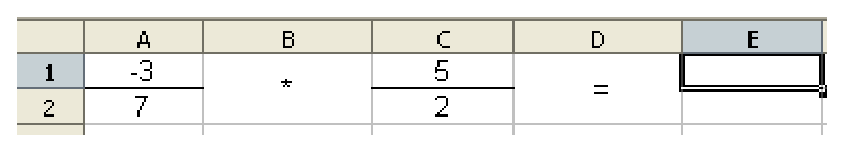
\includegraphics[width=.6\linewidth]{tableur1}
    \end{center}
    
    \begin{itemize}
        \item Recopiez les cellules ci-dessus ;
        \item Dans la cellule E1, tapez « \texttt{=A1*C1} » ;
        \item Dans la cellule E2, tapez « \texttt{=A2*C2} » ;
        \item Utilisez cette feuille de calcul pour vérifier le résultat du calcul B (question a.). Que remarquez-vous ?
    \end{itemize}
    
    \item Sur le même fichier, vous allez maintenant construire un outil permettant de calculer la somme de deux fractions.
    
    \begin{center}
        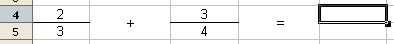
\includegraphics[width=.6\linewidth]{tableur2}
    \end{center}
    
    Recopiez les cellules ci-dessus ;
    Que faut-il taper comme formules dans les cellules E4 et E5 ?
    Utilisez cette feuille de calcul pour vérifier le résultat du calcul D (question a.). Que remarquez-vous ?
    \item Procédez de la même façon pour construire sur le même fichier quatre outils permettant :
    \begin{itemize}
        \item de calculer le produit de trois fractions ;
        \item de calculer la différence de deux fractions ;
        \item de calculer la somme de trois fractions ;
        \item de calculer le quotient de deux fractions.
    \end{itemize}
    \item Construisez un nouvel outil permettant de calculer la somme de deux fractions en faisant apparaître les étapes intermédiaires.
    \item Refaites tous les calculs avec le fichier tableur qui se trouve en complément. Quelle est la nouveauté apportée par ce fichier par rapport au vôtre ?
    \item Dans quels cas, les deux fichiers donnent-ils des résultats identiques ?
\end{enumerate}
\end{TP}

\recreation % avec R majuscule pour saut de page
%\begin{enigme}[Étourdi !]
Un abreuvoir est alimenté par deux robinets. Lorsque le robinet d'évacuation est fermé, le premier robinet seul le remplit en 4 heures. Le deuxième robinet seul le remplit en 3 heures.

\vspace{.5em}

Lorsque l'abreuvoir est plein, le robinet d'évacuation le vide en 2 heures.

\vspace{.5em}

Alors que l'abreuvoir est vide, l'éleveur ouvre les deux robinets pour le remplir,
mais oublie de fermer le robinet d'évacuation !

\vspace{.5em}

L'abreuvoir va-t-il quand même se remplir ?

Si oui, en combien de temps ?
\end{enigme}





\themaG
\chapter{Angles}\label{ChAngles}

\vspace{5cm}
\begin{acquis}
\begin{itemize}
\item Savoir repérer les angles formés par deux parallèles et une sécante (angles alternes-internes, angles alternes-externes, angles correspondants).
\item Savoir calculer des mesures d’angles en utilisant plusieurs propriétés (somme des angles d'un triangle, angles formés par deux parallèles et une sécante…).
\columnbreak
\item Savoir utiliser les propriétés des angles pour prouver que des droites sont parallèles ou perpendiculaires.
\item Savoir résoudre des problèmes en utilisant les angles.
\end{itemize}
\end{acquis}


\activites  
\begin{activite}[Les deux font la paire]



\begin{tabularx}{\linewidth}{XXXX}
\multicolumn{1}{c}{Figure 1} &
\multicolumn{1}{c}{Figure 2} &
\multicolumn{1}{c}{Figure 3} &
\multicolumn{1}{c}{Figure 4} \\
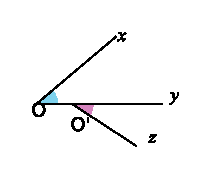
\includegraphics[width=.85\linewidth]{acti1} &

\includegraphics[width=.85\linewidth]{acti2} &
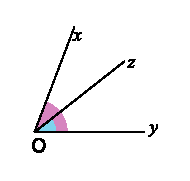
\includegraphics[width=.85\linewidth]{acti3} &
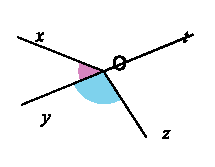
\includegraphics[width=.85\linewidth]{acti4} \\ 
\end{tabularx}

\begin{enumerate}
\item Dans les figures 2 et 4, les angles bleu et rose sont dits \textbf{adjacents}. Ce n'est pas le cas pour les autres figures. À partir de tes observations, essaie d'expliquer à quelles conditions deux angles sont adjacents. 
\item Deux angles adjacents ont-ils nécessairement la même mesure ? Justifie ta réponse.

\vspace{1em}

\begin{tabularx}{\linewidth}{XXXX}
\multicolumn{1}{c}{Figure 5} &
\multicolumn{1}{c}{Figure 6} &
\multicolumn{1}{c}{Figure 7} &
\multicolumn{1}{c}{Figure 8} \\
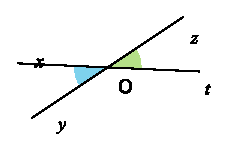
\includegraphics[width=.85\linewidth]{acti5} &

\includegraphics[width=.85\linewidth]{acti6} &
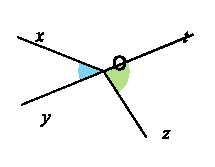
\includegraphics[width=.85\linewidth]{acti7} &
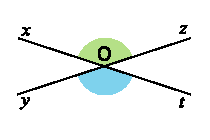
\includegraphics[width=.85\linewidth]{acti8} \\ 
\end{tabularx}

\item Dans les figures 5 et 8, les angles bleu et vert sont dits \textbf{opposés par le sommet}. Ce n'est pas le cas pour les autres figures. À partir de tes observations, essaie d'expliquer à quelles conditions deux angles sont opposés par le sommet.
\item Deux angles opposés par le sommet ont-ils nécessairement la même mesure ? Justifie ta réponse en utilisant une propriété sur deux angles symétriques par rapport à un point.
\end{enumerate}
\end{activite}


\begin{activite}[De jolies sommes !]
\begin{enumerate} \item Trace un triangle $ABC$ rectangle en $A$ puis mesure les angles $\widehat{ABC}$ et $\widehat{BCA}$.
\item Marie affirme que tous les élèves de la classe ne trouveront pas nécessairement les mêmes mesures mais qu'il y a quand même une relation entre ces deux mesures. Quelle est-elle ? Justifie ta réponse.

\vspace{1em}

On dit que deux angles sont \textbf{complémentaires} lorsque la somme de leurs mesures est égale à 90°. 
\item Les angles $\widehat{ABC}$ et $\widehat{BCA}$ sont-ils complémentaires ?
\item  Construis deux angles complémentaires \textbf{et} adjacents dont l'un mesure 64°.
\item Ahmed a mesuré l'angle $\widehat{xOz}$ ci-dessous et a trouvé 110°.

\begin{center}
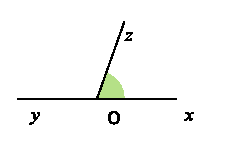
\includegraphics[width=.25\linewidth]{acti9}
\end{center}

Sa voisine lui dit que ce n'est pas possible et qu'à partir de l'erreur d'Ahmed elle pense connaître la bonne mesure. Quelle est cette mesure ? Comment a-t-elle pu la trouver ?

\vspace{1em}

On dit que deux angles sont \textbf{supplémentaires} lorsque la somme de leurs mesures est égale à 180°. 
\item Les angles $\widehat{xOz}$ et $\widehat{zOy}$ sont-ils supplémentaires ?
\item Construis deux angles supplémentaires \textbf{et} non adjacents dont l'un mesure 52°.
\end{enumerate}
\end{activite}


\begin{activite}[Avec des angles correspondants égaux...]
\begin{enumerate}
\item Observe la figure ci-dessous puis reproduis-la en choisissant la même mesure pour les angles $\widehat{ERF}$ et $\widehat{ESH}$.

\begin{center}
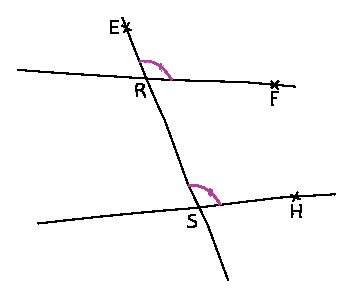
\includegraphics[width=.25\linewidth]{acti10}
\end{center}

\item\label{AactiquestionAngles} Comment peux-tu qualifier les angles $\widehat{ERF}$ et $\widehat{ESH}$ ? 
\item\label{AactiquestionDroites} Sur ta figure, quelle est la position relative des droites $(RF)$ et $(SH)$ ?
\item\label{AactiquestionPhrase} À l'aide des questions \ref{AactiquestionAngles} et \ref{AactiquestionDroites}, recopie puis complète la phrase : \textsl{« Si deux angles correspondants sont ... alors les deux droites coupées par la sécante sont ... . »}.
\item Écris une propriété identique à celle de la question \ref{AactiquestionPhrase} pour les angles alternes-internes.
\end{enumerate}
\end{activite}

\cours

\section{Caractériser deux angles ayant un sommet commun}

\begin{aconnaitre}
\textbf{Deux angles adjacents} sont deux angles qui ont un sommet commun, un côté commun et qui sont situés de part et d'autre de ce côté commun.

\vspace{.5em}

\textbf{Deux angles opposés par le sommet} sont deux angles qui ont un sommet commun et qui ont leurs côtés dans le prolongement l'un de l'autre.
\end{aconnaitre}

\begin{exemple*1}

Sur la figure ci-dessous, que peux-tu dire des angles $\widehat{AOB}$ et $\widehat{BOC}$ ?

\begin{center}
    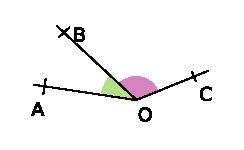
\includegraphics[width=.25\linewidth]{cours1}
\end{center}

\correction
Les angles $\widehat{AOB}$ et $\widehat{BOC}$ ont comme sommet commun le point $O$, comme côté commun la demi-droite $[OB)$ et sont placés de part et d'autre de $[OB)$ : ils sont donc adjacents.
\end{exemple*1}


\begin{exemple*1}
Sur la figure ci-dessous, que peux-tu dire des angles $\widehat{AOB}$ et $\widehat{DOE}$ ?

\begin{center}
    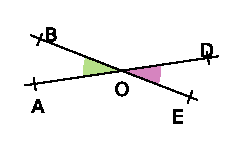
\includegraphics[width=.25\linewidth]{cours2}
\end{center}

\correction
Les angles $\widehat{AOB}$ et $\widehat{DOE}$ ont comme sommet commun le point $O$ et des côtés dans le prolongement l'un de l'autre ($A$, $O$, $D$ et $B$, $O$, $E$ sont alignés) : ils sont donc opposés par le sommet.
\end{exemple*1}

\vspace{1em}

Exercices « À toi de jouer »

Sur la figure ci-dessous, nomme trois paires d'angles adjacents.

\begin{center}
    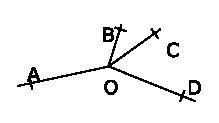
\includegraphics[width=.2\linewidth]{cours3}
\end{center}

Que dire des angles $\widehat{VST}$ et $\widehat{ESR}$ pour un parallélogramme $VERT$ de centre $S$ ?


\begin{aconnaitre}
Si deux angles sont opposés par le sommet \textbf{alors ils ont la même mesure.}
\end{aconnaitre}



\section{Angles complémentaires et supplémentaires}

\begin{aconnaitre}
\textbf{Deux angles complémentaires} sont deux angles dont la somme des mesures est égale à 90°.

\vspace{.5em}

\textbf{Deux angles supplémentaires} sont deux angles dont la somme des mesures est égale à 180°.
\end{aconnaitre}

\begin{exemple*1}
Sur la figure ci-dessous, que peux-tu dire des angles $\widehat{AOB}$ et $\widehat{BOC}$ ?

\begin{center}
    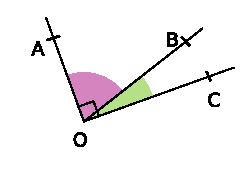
\includegraphics[width=.25\linewidth]{cours4}
\end{center}

\correction
Les angles $\widehat{AOB}$ et $\widehat{BOC}$ forment un angle droit : la somme des mesures de ces angles vaut 90°. Ce sont donc des angles complémentaires.
\end{exemple*1}

\begin{remarque}
Deux angles complémentaires et adjacents forment un angle droit. On peut donc en déduire que des droites sont perpendiculaires.
\end{remarque}


\begin{exemple*1}
Sur la figure ci-dessous, que peux-tu dire des angles $\widehat{AOB}$ et $\widehat{FED}$ ?

\begin{center}
    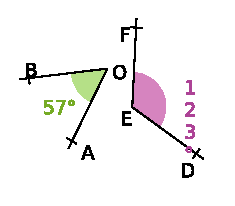
\includegraphics[width=.25\linewidth]{cours5}
\end{center}

\correction
$\widehat{AOB}+\widehat{FED}=57^\circ+123^\circ=180^\circ$ donc les angles $\widehat{AOB}$ et $\widehat{FED}$ sont supplémentaires.
\end{exemple*1}

\begin{remarque}
Deux angles supplémentaires et adjacents forment un angle plat. On peut donc en déduire que des points sont alignés.
\end{remarque}

\begin{remarque}
Deux angles complémentaires ou supplémentaires ne sont pas forcément adjacents.
\end{remarque}

\vspace{1em}

Exercices « À toi de jouer »

Les angles ci-dessous sont-ils complémentaires ?

\begin{center}
    
\includegraphics[width=.2\linewidth]{cours6}
\end{center}

Donne le complémentaire d'un angle de 27°.

Que peux-tu dire des angles aigus d'un triangle rectangle ? Justifie ta réponse.


Les angles ci-dessous sont-ils supplémentaires ?
\begin{center}
    
\includegraphics[width=.2\linewidth]{cours7}
\end{center}


Les points A, O et B sont-ils alignés ?
\begin{center}
    
\includegraphics[width=.2\linewidth]{cours8}
\end{center}







\section{Caractériser deux angles définis par deux droites et une sécante}


\begin{aconnaitre}
\begin{minipage}{.3\linewidth}
\centering

\includegraphics[width=.65\linewidth]{cours9}
\end{minipage}\hfill%
\begin{minipage}{.67\linewidth}
Les angles verts sont \textbf{alternes-internes}.

Ils sont déterminés par les droites $(d)$, $(d')$ et la sécante $(d_1)$.

Les angles roses sont \textbf{correspondants.}

Ils sont déterminés par les droites $(d)$, $(d')$ et la sécante $(d_2)$.
\end{minipage}
\end{aconnaitre}

\begin{exemple*1}
À l'aide de la figure, nomme des angles alternes-internes et des correspondants.

\begin{center}
    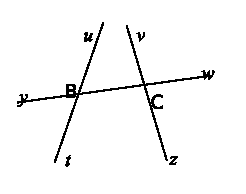
\includegraphics[width=.25\linewidth]{cours10}
\end{center}

\correction
Les droites $(ut)$, $(vz)$ et la sécante $(yw)$ forment :
\begin{itemize}
    \item deux paires d'angles alternes-internes qui sont : $\widehat{uBw}$ et $\widehat{yCz}$, $\widehat{vCy}$ et $\widehat{tBw}$.
    \item quatre paires d'angles correspondants qui sont : $\widehat{yBu}$ et $\widehat{vCy}$, $\widehat{yBt}$ et $\widehat{yCz}$, $\widehat{uBw}$ et $\widehat{vCw}$, $\widehat{tBw}$ et $\widehat{zCw}$.
\end{itemize}
\end{exemple*1}

\vspace{1em}

Exercices « À toi de jouer »

Sur la figure ci-dessous, les angles $\widehat{yOx'}$ et $\widehat{xEz'}$ sont-ils alternes-internes ? Justifie.

\begin{center}
    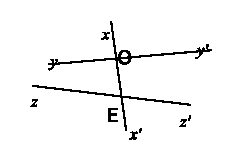
\includegraphics[width=.2\linewidth]{cours11}
\end{center}

Sur la figure  ci-dessous, nomme deux paires d'angles alternes-internes et quatre paires d'angles correspondants.

\begin{center}
    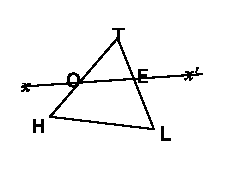
\includegraphics[width=.2\linewidth]{cours12}
\end{center}

\begin{aconnaitre}
Si deux angles alternes-internes sont déterminés par des droites parallèles \textbf{alors ils ont la même mesure.}

\vspace{.5em}

Si deux angles correspondants sont déterminés par des droites parallèles \textbf{alors ils ont la même mesure}.
\end{aconnaitre}

\begin{exemple*1}
Les droites $(vt)$ et $(uy)$ sont parallèles. Calcule la mesure des angles $\widehat{zEy}$ et $\widehat{vGw}$.

\begin{center}
    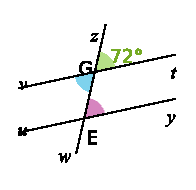
\includegraphics[width=.25\linewidth]{cours13}
\end{center}

\correction
Les angles correspondants $\widehat{zGt}$ et $\widehat{zEy}$ sont déterminés par les droites $(vt)$ et $(uy)$ qui sont parallèles. Ils sont donc de la même mesure. L'angle $\widehat{zEy}$ mesure donc 72°.

\vspace{.5em}

Les angles $\widehat{zGt}$ et $\widehat{vGw}$ sont opposés par le sommet. Ils sont donc de la même mesure. L'angle $\widehat{vGw}$ mesure donc 72°.
\end{exemple*1}

\vspace{1em}

Exercice « À toi de jouer »

Sur la figure ci-contre, les droites $(zz')$ et $(uu')$ sont parallèles. Calcule la mesure de l'angle $\widehat{x'Rz'}$ puis celle de l'angle $\widehat{uEx}$.

\begin{center}
    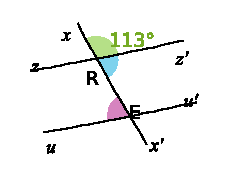
\includegraphics[width=.3\linewidth]{cours14}
\end{center}


\begin{aconnaitre}
Si deux angles alternes-internes sont de même mesure \textbf{alors les deux droites coupées par la sécante sont parallèles.}

\vspace{.5em}

Si deux angles correspondants sont de même mesure \textbf{alors les deux droites coupées par la sécante sont parallèles.}
\end{aconnaitre}


\begin{exemple*1}
Les droites $(yy')$ et $(zz')$ sont-elles parallèles ? Les droites $(xx')$ et $(uu')$ sont-elles parallèles ?

\begin{center}
    
\includegraphics[width=.3\linewidth]{cours15}
\end{center}

\correction
Les angles $\widehat{x'Ay'}$ et $\widehat{xBz}$ déterminés par les droites $(yy')$, $(zz')$ et la sécante $(xx')$ sont alternes-internes. Les angles $\widehat{x'Ay'}$ et $\widehat{xBz}$ ont la même mesure.

Donc les droites $(yy')$ et $(zz')$ sont parallèles.

\vspace{.5em}

Les angles $\widehat{x'Ay'}$ et $\widehat{u'Dy'}$ déterminés par les droites $(xx')$, $(uu')$ et la sécante $(yy')$ sont correspondants. Si les droites $(xx')$ et $(uu')$ étaient parallèles alors les angles $\widehat{x'Ay'}$ et $\widehat{u'Dy'}$ seraient de la même mesure, ce qui n'est pas le cas.

Donc les droites $(xx')$ et $(uu')$ ne sont pas parallèles.
\end{exemple*1}

\vspace{1em}

Exercice « À toi de jouer »

Dans chacun des cas ci-dessous, indique si les droites $(AB)$ et $(OT)$ sont parallèles. Justifie ta réponse.

\begin{center}
\begin{minipage}{.48\linewidth}
\centering
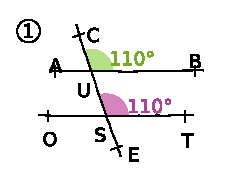
\includegraphics[width=.45\linewidth]{cours16}
\end{minipage}\hfill%
\begin{minipage}{.48\linewidth}
\centering
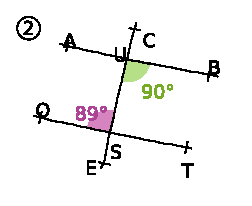
\includegraphics[width=.45\linewidth]{cours17}
\end{minipage}
\end{center}


\exercicesbase
\begin{colonne*exercice}
\serie{Propriétés des triangles}


\begin{exercice}[Reconnaître]
Donne, en justifiant, la nature de chacun des triangles s'il est particulier.
\begin{colenumerate}{4}
\item 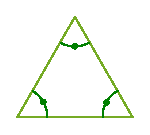
\includegraphics[width=.8\linewidth]{exoEnt1}
\item 
\includegraphics[width=.8\linewidth]{exoEnt2}
\item 
\includegraphics[width=.8\linewidth]{exoEnt3}
\item 
\includegraphics[width=.8\linewidth]{exoEnt4}
\end{colenumerate}
\end{exercice}



\begin{exercice}
Dans chaque cas, effectue un croquis puis construis la figure.
\begin{colenumerate}{1}
\item Trace un triangle $FIN$ rectangle en $F$ tel que $FI$ = 5 cm et $NF$ = 6 cm.
\item Trace un triangle $TRS$ rectangle en $S$ tel que $TS$ = 72 mm et $SR$ = 85 mm.
\item Construis un triangle $MNO$ équilatéral de côté 5 cm.
\item Construis un triangle isocèle $STU$ isocèle en $S$ tel que $ST$ = 58 mm et $TU$ = 32 mm.
\item Construis un triangle $ABC$ tel que $AB$ = 6 cm ; $BC$ = 5,2 cm et $CA$ = 42 mm.
\end{colenumerate}
\end{exercice}



\begin{exercice}[Médiatrices dans un triangle]
\begin{enumerate}
\item Construis un triangle $ABC$ tel que $AB$ = 5,7 cm, $AC$ = 5,3 cm et $BC$ = 7 cm.
\item Construis les médiatrices des segments $[AB]$ et $[CB]$. Note $O$ leur point d'intersection.
\item Construis la médiatrice du segment $[AC]$. Que constates‑tu ?
\item Trace le cercle de centre $O$ passant par $A$. Comment s'appelle ce cercle ?
\end{enumerate}
\end{exercice}



\begin{exercice}[Bissectrice dans un triangle]
\begin{enumerate}
\item Trace un triangle $UST$ tel que $UT$ = 6 cm ; $US$ = 10 cm et $ST$ = 14 cm.
\item Construis les bissectrices des angles $\widehat{UST}$, $\widehat{UTS}$ et $\widehat{TUS}$.

Que constates‑tu ?
\end{enumerate}
\end{exercice} 




\begin{exercice}
Dans les 6 cas suivants, détermine si la droite $d$ est :
\begin{enumerate}
\item une hauteur ;
\item une médiatrice ;
\item une bissectrice ;
\item une médiane.
\end{enumerate}

\begin{colenumerate}{3}
\item 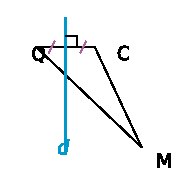
\includegraphics[width=.8\linewidth]{exoEnt5}
\item 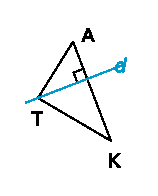
\includegraphics[width=.8\linewidth]{exoEnt6}
\item 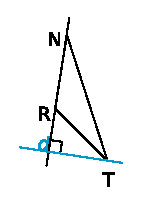
\includegraphics[width=.8\linewidth]{exoEnt7}
\item 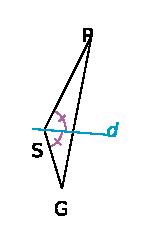
\includegraphics[width=.8\linewidth]{exoEnt8}
\item 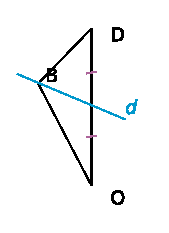
\includegraphics[width=.8\linewidth]{exoEnt9} 
\item 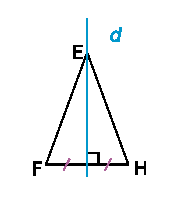
\includegraphics[width=.8\linewidth]{exoEnt10}
\end{colenumerate}
\end{exercice}




\begin{exercice}[Vocabulaire]
\begin{enumerate}
\item Construis un triangle $BOA$ tel que $BO$ = 5 cm, $OA$ = 7 cm et $AB$ = 8 cm. Trace la droite $d_1$ perpendiculaire à $[BO]$ et passant par $A$.
\item Trace la droite $d_2$ perpendiculaire au segment $[OA]$ et passant par son milieu.
\item Trace la droite $d_3$ qui coupe l'angle $\widehat{OBA}$ en deux angles égaux.
\item Trace la droite $d_4$ qui passe par $O$ et par le milieu de $[BA]$.
\item Détermine quelle(s) droite(s) représente(nt) la hauteur du triangle.
\item Détermine quelle(s) droite(s) représente(nt) une médiatrice.
\item Détermine quelle(s) droite(s) représente(nt) une bissectrice.
\item Détermine quelle(s) droite(s) représente(nt) une médiane.
\end{enumerate}
\end{exercice}




\begin{exercice}[Hauteurs d'un triangle]
Construis un triangle $BON$ tel que $BO$ = 68 mm, $BN$ = 62 mm et $NO$ = 45 mm.

Trace :
\begin{itemize}
\item en noir, la perpendiculaire à $(BN)$ passant par $O$ ;
\item en rouge, la perpendiculaire à $(NO)$ passant par $B$ ;
\item en vert, la perpendiculaire à $(BO)$ passant par $N$. Que remarques‑tu ?
\end{itemize}
\end{exercice}


\begin{exercice}[Hauteur (« relative à » ou « issue de »)]
\begin{enumerate}
\item Construis un triangle $AVE$ quelconque puis trace :
    \begin{itemize}
    \item en bleu, la hauteur issue du sommet $E$ ;
    \item en noir, la hauteur issue du sommet $A$ ;
    \item en rouge, la hauteur relative à $[AE]$.
    \end{itemize}
\item Observe ces trois hauteurs. Quelle remarque peux-tu faire ?
\end{enumerate}
\end{exercice}



\begin{exercice}[À l'intérieur ou pas ?]
\begin{enumerate}
\item Construis un triangle $DER$ ayant tous ses angles aigus. Trace les hauteurs de ce triangle.
\item Construis un triangle $NRV$ tel que $\widehat{NRV}$ soit un angle obtus. Trace les hauteurs de ce triangle.
\item Construis un triangle $GHT$ rectangle en $T$. Trace les hauteurs de ce triangle.
\item Observe les trois figures. Quelles remarques peux-tu faire ?
\end{enumerate}
\end{exercice}



\begin{exercice}[Vocabulaire] 
\begin{enumerate}
\item Construis un triangle $OA$. Trace la droite $(d_1)$ perpendiculaire à $[BO]$ et passant par $A$.
\item Trace la droite $(d_2)$ perpendiculaire au segment $[OA]$ et passant par son milieu.
\item Trace la droite $(d_3)$ qui coupe l'angle $\widehat{BOA}$ en deux angles égaux.
\item Trace la droite $(d_4)$ qui passe par $O$ et par le milieu de $[BA]$.
\item Reformule les questions précédentes en utilisant les mots : médiatrice, bissectrice, médiane et hauteur.
\end{enumerate}
\end{exercice}



\begin{exercice}[Cercles circonscrits]
Dans chaque cas, construis le triangle $LYS$ puis son cercle circonscrit.
\begin{enumerate}
\item $LS$ = 8 cm, $\widehat{YLS}$ = 65° et $\widehat{YSL}$ = 45°.
\item $LS$ = 4 cm, $LY$ = 5 cm et $\widehat{YLS}$ = 103°.
\item $LYS$ est isocèle en $L$ tel que $LY$ = 8 cm et $YS$ = 5,5 cm.
\item $LYS$ est un triangle équilatéral de côté 6 cm.
\end{enumerate}
\end{exercice}




\begin{exercice}[Sois malin !]
\begin{enumerate}
\item Construis un triangle $MEC$ tel que son cercle circonscrit ait un rayon de 5 cm.
\item Construis un triangle $RNB$ isocèle en $B$ avec $BN$ = 4 cm tel que son cercle circonscrit ait un rayon de 5 cm.
\end{enumerate}
\end{exercice}



\begin{exercice}[Cercle inscrit]
Dans chaque cas, construis le triangle $ABC$ puis son cercle inscrit.
\begin{enumerate}
\item $AC$ = 8 cm, $\widehat{BAC}$ = 60° et $\widehat{ACB}$ = 50°.
\item $AC$ = 10 cm, $AB$ = 8 cm et $\widehat{BAC}$ = 45°.
\item $ABC$ est isocèle en $A$ tel que $AB$ = 9 cm et $BC$ = 6 cm.
\item $ABC$ est un triangle équilatéral de côté 7,5 cm.
\end{enumerate}
\end{exercice}



\serie{Utiliser le vocabulaire associé aux angles}






\begin{exercice}
$\hat{a}$ et $\hat{b}$ sont deux angles complémentaires.

Calcule la mesure de $\hat{b}$ si :

$\hat{a}$ = 45°,\hfill%
$\hat{a}$ = 37°,\hfill%
$\hat{a}$ = 2°,\hfill%
$\hat{a}$ = 88,3°.  
\end{exercice}



\begin{exercice}
$\hat{x}$ et $\hat{y}$ sont deux angles supplémentaires.

Calcule la mesure de $\hat{y}$ si :

$\hat{x}$= 103°,\hfill%
$\hat{x}$= 95°,\hfill%
$\hat{x}$= 56°,\hfill%
$\hat{x}$= 0,3°.
\end{exercice}




\begin{exercice}
Indique si les angles proposés sont adjacents, complémentaires ou bien encore supplémentaires. Justifie tes réponses. 

\begin{center}
    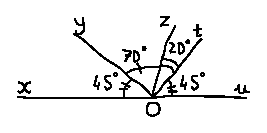
\includegraphics[width=.8\linewidth]{exoEnt11}
\end{center}

\begin{enumerate}
\item $\widehat{yOz}$ et $\widehat{zOt}$ ;
\item $\widehat{xOy}$ et $\widehat{yOu}$ ;
\item $\widehat{xOy}$ et $\widehat{tOu}$ ;
\item $\widehat{yOu}$ et $\widehat{tOu}$ ;
\item $\widehat{xOz}$ et $\widehat{zOt}$ ;
\item $\widehat{xOt}$ et $\widehat{uOt}$.
\end{enumerate}
\end{exercice}


\columnbreak
\begin{exercice}[Les deux font la paire]
Nomme, en justifiant, deux angles de la figure, codés ou non :
\begin{enumerate}
\item complémentaires et adjacents ;
\item complémentaires et non adjacents ;
\item supplémentaires et adjacents ;
\item supplémentaires et non adjacents ;
\item opposés par le sommet.
\end{enumerate}

\begin{center}
    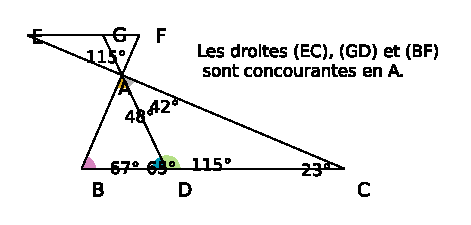
\includegraphics[width=\linewidth]{exoEnt12}
\end{center}

\end{exercice}




\begin{exercice}[Les angles inconnus]
\begin{enumerate}
\item Trouve la mesure de deux angles complémentaires, sachant que l'un d'eux est 8 fois plus grand que l'autre.
\item Trouve la mesure de deux angles supplémentaires, sachant que l'un d'eux est 9 fois plus petit que l'autre.
\end{enumerate}
\end{exercice}



\begin{exercice}[Des angles dynamiques...]
\begin{enumerate}
\item À l'aide du logiciel \emph{TracenPoche}, construis deux angles complémentaires et adjacents.
\item Propose une façon de procéder pour que ces angles restent adjacents, complémentaires et égaux à 45°, même quand on bouge les points.
\end{enumerate}
\end{exercice}



\begin{exercice}
Que peut-on dire des angles :

\begin{minipage}{.3\linewidth}
\begin{enumerate}
\item 1 et 3 ?
\item 1 et 5 ?
\item 3 et 5 ?
\item 1 et 4 ?
\item 4 et 6 ?
\item 3 et 7 ?
\end{enumerate}
\end{minipage}\hfill%
\begin{minipage}{.67\linewidth}
\centering
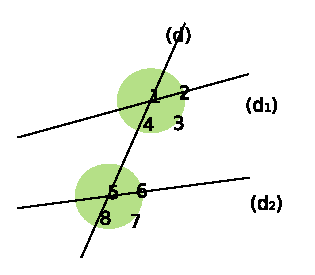
\includegraphics[width=\linewidth]{exoEnt13}
\end{minipage}
\end{exercice}




\begin{exercice}
Nomme deux angles de la figure et précise le nom de la sécante correspondante :
\begin{enumerate}
\item alternes-internes avec l'angle \no 3 ;
\item correspondants avec l'angle \no 10 ;
\item alternes-internes avec l'angle \no 13 ;
\item correspondants avec l'angle \no 7.
\end{enumerate}

\begin{center}
    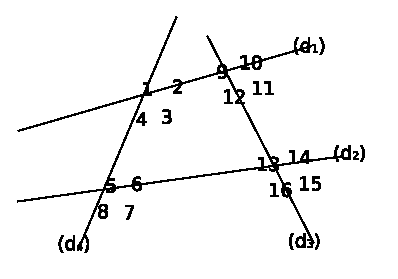
\includegraphics[width=.8\linewidth]{exoEnt14}
\end{center}

\end{exercice}



\begin{exercice}[Recherche de mesures d'angles]
\begin{enumerate}
\item Nomme deux paires d'angles de la figure :
    \begin{itemize}
    \item alternes-internes aigus ;
    \item alternes-internes de même mesure ;
    \item correspondants aigus ;
    \item supplémentaires et non adjacents.
    \end{itemize}
    
\begin{center}
    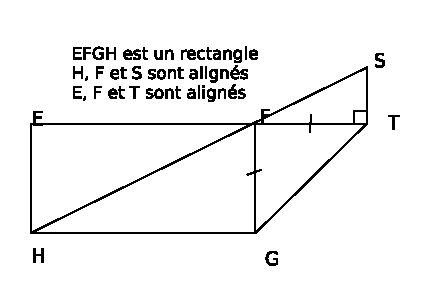
\includegraphics[width=.9\linewidth]{exoEnt15}
\end{center}

\item Sachant de plus que $\widehat{EFH}$ = 27°, calcule la mesure de l'angle $\widehat{SFT}$ puis celle de $\widehat{SFG}$.
\end{enumerate}
\end{exercice}

\columnbreak
\serie{Caractériser des droites parallèles par les angles}



\begin{exercice}
Dans chaque cas, dire si les droites $(d_1)$ et $(d_2)$ sont ou non parallèles et pourquoi.
\begin{center}
    \includegraphics[width=.8\linewidth]{exoEnt16}
\end{center}
\end{exercice} 



\begin{exercice}[Le coup des équerres !]
Arnaud a placé ses deux équerres identiques sur la droite $(d)$ comme l'illustre le schéma ci-dessous.

\begin{center}
    \includegraphics[width=.8\linewidth]{exoEnt17}
\end{center}

\begin{enumerate}
\item Il affirme que, de cette façon, il peut tracer des droites parallèles. Est-ce vrai et pourquoi ?
\item Quelles seraient les autres façons de positionner les équerres pour obtenir le même résultat ?
\end{enumerate}
\end{exercice} 



\begin{exercice}[Angles et droites parallèles]

\begin{center}
    \includegraphics[width=.8\linewidth]{exoEnt18}
\end{center}

\begin{enumerate}
\item Calcule la mesure de l'angle $\widehat{uBr}$.
\item Les droites $(xy)$ et $(sr)$ sont-elles parallèles ? Justifie ta réponse.
\end{enumerate}
\end{exercice}



\columnbreak
\serie{Calculer des angles formés par des\\ droites parallèles}





\begin{exercice}[Parallèles ?]
Sur la figure ci-dessous, les angles $\widehat{BAE}$ et $\widehat{FEO}$ sont égaux à 58°.

\begin{center}
    \includegraphics[width=.7\linewidth]{exoEnt19}
\end{center}

\begin{enumerate}
\item Que peux-tu dire des droites $(EF)$ et $(AB)$ ? Justifie ta réponse.
\item On sait de plus que la mesure de l'angle $\widehat{FBA}$ est 45°. Déduis-en la mesure de l'angle $\widehat{OFE}$. Justifie ta réponse.
\end{enumerate}
\end{exercice}


\begin{exercice}[Droites parallèles]

\begin{center}
    \includegraphics[width=.7\linewidth]{exoEnt20}
\end{center}

Sur la figure ci-dessus, les droites $(xy)$ et $(zt)$ sont parallèles. L'angle $\widehat{xMu}$ vaut 125°.
\begin{enumerate}
\item Donne la mesure de l'angle $\widehat{vMy}$. Justifie ta réponse.
\item Donne d'autres angles dont la mesure est de 125°. Justifie ta réponse.
\end{enumerate}
\end{exercice}

\newpage
\begin{exercice}[Angles supplémentaires]
                        
\begin{center}
    \includegraphics[width=\linewidth]{exoEnt21}
\end{center}
                                 
\begin{enumerate}
\item Justifie que les angles $\widehat{BAC}$ et $\widehat{BDC}$ sont de même mesure.
\item Que dire des angles $\widehat{BDC}$ et $\widehat{BDE}$ ? Pourquoi ? Justifie alors que les deux angles marqués sont supplémentaires.
\end{enumerate}
\end{exercice}

\columnbreak
\begin{exercice}[Zigzag]

\begin{center}
    \includegraphics[width=.8\linewidth]{exoEnt22}
\end{center}

Sur la figure ci-dessus :
\begin{itemize}
    \item les droites $(AB)$, $(CD)$ et $(EF)$ sont parallèles ;
    \item $R$ est un point de la droite $(AB)$, $S$ est un point de la droite $(CD)$ et $T$ est un point de la droite $(EF)$ tels que : $\widehat{BRS}$ = 20° et $\widehat{RST}$ = 57°.
\end{itemize}

Calcule la mesure de l'angle $\widehat{STF}$.
\end{exercice}


\begin{exercice}
Construis à l'aide de \emph{TracenPoche} un quadrilatère $EFGH$ ayant deux angles droits, en $E$ et en $G$.
\begin{enumerate}
\item Affiche la mesure des angles $\widehat{EFG}$ et $\widehat{EHG}$. Que remarques-tu ?
\item Trace le segment $[FH]$. En raisonnant dans les triangles $EFH$ et $FHG$, démontre que $\widehat{EFG}$ et $\widehat{EHG}$ sont supplémentaires.
\end{enumerate}
\end{exercice}

\end{colonne*exercice}


\exercicesappr
\begin{colonne*exercice}
\begin{exercice}
Dans chaque cas, précise si les droites $(d_1)$ et $(d_2)$ sont ou non parallèles et pourquoi.

\begin{center}
    \includegraphics[width=\linewidth]{exoApp1}
\end{center}

\end{exercice}



\begin{exercice}[Triangle isocèle]

\begin{center}
    \includegraphics[width=.8\linewidth]{exoApp2}
\end{center}

La figure ci-dessus est telle que :
\begin{itemize}
    \item $B$, $A$ et $D$ sont des points alignés ;
    \item $\widehat{BAC}$ et $\widehat{ACD}$ sont supplémentaires ;
    \item $\widehat{BAC}$= 110°.
\end{itemize}

\begin{enumerate}
\item Montre, en justifiant, que les angles $\widehat{DAC}$ et $\widehat{ACD}$ sont égaux à 70°.
\item Montre alors que le triangle $ADC$ est isocèle.
\item De plus, l'angle $\widehat{ACB}$ mesure 50°. Montre, en justifiant, que les angles $\widehat{BCA}$ et $\widehat{ADC}$ sont complémentaires.
\item Trouve, en justifiant, deux autres paires d'angles complémentaires.
\end{enumerate}
\end{exercice}




\begin{exercice}[Parallèles ou non ?]

\begin{center}
    \includegraphics[width=.8\linewidth]{exoApp3}
\end{center}

La figure ci-dessus est tracée à main levée.

\begin{enumerate}
\item Calcule la mesure de l'angle $\widehat{LON}$.
\item Déduis-en la mesure de l'angle $\widehat{ONL}$.
\item Détermine alors si les droites $(LN)$ et $(MP)$ sont parallèles.
\item Sachant que les segments $[LN]$ et $[MP]$ sont de même longueur, détermine la nature du quadrilatère $LNPM$.
\end{enumerate}
\end{exercice}




\begin{exercice}[Un isocèle de plus]

\begin{center}
    \includegraphics[width=.6\linewidth]{exoApp4}
\end{center}

La figure ci-dessus est telle que :
\begin{itemize}
    \item les droites $(RO)$ et $(SN)$ sont sécantes en $T$ ;
    \item le triangle $RST$ est isocèle en $R$ ;
    \item les droites $(RS)$ et $(NO)$ sont parallèles.
\end{itemize}

Montre que le triangle $TNO$ est isocèle.
\end{exercice}




\begin{exercice}[Un périscope de fortune !]

\begin{enumerate}
\item Fais une recherche sur Internet concernant la loi de réflexion de la lumière.
\item Le schéma ci-dessous illustre un rayon de lumière qui se réfléchit sur un miroir avec un angle de 30°. Détermine $\hat{x}$ et $\hat{y}$. Justifie.

\begin{center}
    \includegraphics[width=.8\linewidth]{exoApp5}
\end{center}

\item Éric a construit un périscope avec une boîte de carton et deux miroirs parallèles comme l'illustre le schéma ci-dessous.

\begin{center}
    \includegraphics[width=.8\linewidth]{exoApp6}
\end{center}

\begin{itemize}
    \item Si un rayon entre horizontalement dans le périscope, en sortira-t-il horizontalement aussi ?
    
    (Tu pourras montrer que les rayons d'entrée et de sortie sont parallèles.)
    \item Ce résultat dépend-il de l'inclinaison des miroirs parallèles ?
    
    (Autrement dit, a-t-on le même résultat si l'angle formé par le rayon et le miroir est différent de 45° ?)
\end{itemize}
\end{enumerate}
\end{exercice}

\end{colonne*exercice}

\connaissances
\QCMautoevaluation{Pour chaque question, plusieurs réponses sont proposées. Déterminer celles qui sont correctes.}

\begin{QCM}

\begin{GroupeQCM}


\begin{exercice}
Parmi les couples d'angles suivants, quels sont ceux qui sont complémentaires ?
\begin{ChoixQCM}{2}
\item $\widehat{FEG}=8$° et $\widehat{HIK}=82$°
\item $\widehat{FEG}=90$° et $\widehat{HIK}=90$°
\item $\widehat{ABC}=73$° et $\widehat{STU}=107$°
\item $\widehat{FEG}=89,9$° et $\widehat{HIK}=0,1$°
\end{ChoixQCM}
\begin{corrige}
\reponseQCM{a}
\end{corrige}
\end{exercice}
\end{GroupeQCM}



\begin{EnonceCommunQCM}
Les questions \RefQCM{Aqcm1} et \RefQCM{Aqcm2} se rapportent à la figure ci-dessous.
\begin{center}
    \includegraphics[width=.25\linewidth]{qcm1}
    
    $E$, $R$ et $I$ sont alignés.
\end{center}
\end{EnonceCommunQCM}

\begin{GroupeQCM}


\begin{exercice}\label{Aqcm1}
Les angles...
\begin{ChoixQCM}{2}
\item $\widehat{ERH}$ et $\widehat{HRI}$ sont supplémentaires
\item $\widehat{FRG}$ et $\widehat{HRI}$ sont adjacents
\item $\widehat{ERG}$ et $\widehat{FRI}$ sont supplémentaires
\item $\widehat{FRG}$ et $\widehat{GRH}$ sont adjacents
\end{ChoixQCM}
\begin{corrige}
\reponseQCM{a}
\end{corrige}
\end{exercice}





\begin{exercice}\label{Aqcm2}
L'angle...
\begin{ChoixQCM}{2}
\item $\widehat{FRG}$ est le complémentaire de $\widehat{GRH}$
\item $\widehat{FRE}$ est le complémentaire de $\widehat{HRI}$
\item $\widehat{ERF}$ est le complémentaire de $\widehat{FRI}$
\item $\widehat{GRH}$ est le complémentaire de $\widehat{HRI}$
\end{ChoixQCM}
\begin{corrige}
\reponseQCM{a}
\end{corrige}
\end{exercice}
\end{GroupeQCM}
\end{QCM}

\begin{QCM}

\begin{EnonceCommunQCM}
Les questions \RefQCM{Aqcm3}, \RefQCM{Aqcm4} et \RefQCM{Aqcm5} se rapportent à la figure ci-dessous.
\begin{center}
    \includegraphics[width=.25\linewidth]{qcm2}
    
    $(AD)$ et $(FH)$ sont parallèles.
\end{center}
\end{EnonceCommunQCM}

\begin{GroupeQCM}

\begin{exercice}\label{Aqcm3}

\begin{ChoixQCM}{2}
\item $\widehat{ACH}$ et $\widehat{BCD}$ sont opposés par le sommet
\item $\widehat{CDF}$ et $\widehat{BCD}$ sont opposés par le sommet
\item $\widehat{ACH}$ et $\widehat{BCD}$ sont adjacents
\item $\widehat{BCD}$ et $\widehat{CHF}$ sont correspondants
\end{ChoixQCM}
\begin{corrige}
\reponseQCM{a}
\end{corrige}
\end{exercice}




\begin{exercice}\label{Aqcm4}

\begin{ChoixQCM}{4}
\item $\widehat{BCD}=100$°
\item $\widehat{BHF}=100$°
\item $\widehat{BCA}=100$°
\item $\widehat{DCH}=100$°
\end{ChoixQCM}
\begin{corrige}
\reponseQCM{a}
\end{corrige}
\end{exercice}




\begin{exercice}\label{Aqcm5}

\begin{ChoixQCM}{4}
\item $\widehat{CDF}=40$°
\item $\widehat{BFH}=50$°
\item $\widehat{DCH}=80$°
\item $\widehat{CDF}=100$°
\end{ChoixQCM}
\begin{corrige}
\reponseQCM{a}
\end{corrige}
\end{exercice}



\begin{exercice}
\begin{center}
    \includegraphics[width=.25\linewidth]{qcm3}
\end{center}
\begin{ChoixQCM}{4}
\item Si les angles roses sont égaux alors $(d)$ et $(d')$ sont parallèles
\item Si $(d)$ et $(d')$ sont parallèles alors les angles roses sont égaux
\item Les angles roses sont correspondants
\item Les angles roses sont alternes-internes
\end{ChoixQCM}
\begin{corrige}
\reponseQCM{a}
\end{corrige}
\end{exercice}


\begin{exercice}
Quelles sont les affirmations vraies ?
\begin{ChoixQCM}{4}
\item $\widehat{OUG}$ et $\widehat{ZKL}$ sont opposés par le sommet
\item Deux angles alternes-internes peuvent être opposés par le sommet
\item Deux angles correspondants peuvent être opposés par le sommet
\item Le supplémentaire d'un angle aigu est obtus
\end{ChoixQCM}
\begin{corrige}
\reponseQCM{a}
\end{corrige}
\end{exercice}




\begin{exercice}
\begin{center}
    \includegraphics[width=.25\linewidth]{qcm4}
    
    $(TR)$ et $(SU)$ sont parallèles et $\widehat{REA}$=60°.
\end{center}
\begin{ChoixQCM}{4}
\item $\widehat{EAS}=60$°
\item $\widehat{TEA}=120$°
\item $\widehat{EAU}=60$°
\item $\widehat{EAU}=90$°
\end{ChoixQCM}
\begin{corrige}
\reponseQCM{a}
\end{corrige}
\end{exercice}

\end{GroupeQCM}
\end{QCM}

\TravauxPratiques
\begin{TP}[Triominos avec les angles]


\textbf{1\up{ère} étape : calculer et justifier}

\begin{enumerate}
\item Voici six figures. Pour chacune d'elles, calculez, en justifiant votre calcul, l'angle marqué par un point d'interrogation. (Les droites d'une même couleur sont parallèles.)

\begin{center}
    \includegraphics[width=.6\linewidth]{tabImage}
\end{center}


\item Voici six énoncés. Pour chacun d'eux, répondez à la question en justifiant la réponse :

\begin{center}
    \includegraphics[width=.6\linewidth]{tabType}
\end{center}


\vspace{1em}\textbf{2\up{e} étape : construction des triominos}\vspace{1em}

\item \label{AtpTabType} Voici un tableau qui va vous permettre de construire le jeu de triominos. 

\begin{center}
    \includegraphics[width=.6\linewidth]{tableau}
\end{center}

Toutes les cases d'une même colonne renvoient à l'angle indiqué en ligne 1. Par exemple, les cases F2, F3... renvoient à un angle de 110°.

Pour le type \textbf{t3}, mettez aussi des exemples d'angles correspondants.

\item Dans une feuille blanche au format A4, construisez 10 triangles équilatéraux de 9 cm de côté. Utilisez une seconde feuille pour obtenir 20 triominos au total. Complétez chacun d'eux avec les énoncés ou constructions indiqués dans le tableau de la question \ref{AtpTabType}. en respectant l'ordre donné ci-dessous. Pour vous aider, voici un exemple pour le premier triomino de la série :

\hfill\includegraphics[width=.15\linewidth]{tp7} \hfill \includegraphics[width=.3\linewidth]{tp8}\hfill\phantom{.}
 
\begin{center}
    \includegraphics[width=.75\linewidth]{tp9}
    
    \includegraphics[width=.75\linewidth]{tp10}
\end{center}

\vspace{1em}\textbf{3\up{e} étape : par équipe de deux joueurs}\vspace{1em}

Retournez tous les triominos pour former la pioche. Chaque joueur en prend quatre.      

Un triomino est tiré dans la pioche pour servir de départ. Chaque joueur place à son tour un triomino. (Les côtés qui se touchent doivent correspondre à des angles égaux.)

Si le joueur ne peut pas jouer, il passe son tour \textbf{et} pioche. Le premier joueur qui n'a plus de triomino est déclaré vainqueur.

\textbf{Attention} : si un joueur se trompe en plaçant un triomino, il doit le reprendre et tirer un triomino supplémentaire dans la pioche ; c'est alors à son adversaire de jouer...
\end{enumerate}

\end{TP}

\recreation % avec R majuscule pour saut de page
\begin{enigme}[Un problème de construction]
Trace une droite $(d)$ et place un point $A$ n'appartenant pas à $(d)$.

Construis un triangle équilatéral dont un des sommets est $A$ et les deux autres sommets sont deux points de la droite $(d)$.

Propose une méthode de construction à l'aide d'un logiciel de géométrie dynamique.
\end{enigme}




\themaC
\chapter{Puissances et\\grandeurs}\label{ChPuissances}

\vspace{5cm}
\begin{acquis}
\begin{itemize}
\item Savoir calculer la puissance d'un nombre entier relatif.
\item Savoir utiliser les formules de calcul avec les puissances.
\item Savoir calculer avec les puissances de 10.
\item Savoir résoudre des problème en utilisant les puissances.
\end{itemize}
\end{acquis}


\activites  
\begin{activite}[Le triangle de Sierpinski]

\begin{partie}[Répondre avec des 3 et des $\times$ uniquement !]

\begin{minipage}{.62\linewidth}
La figure de départ est un triangle équilatéral violet. On construit à l'intérieur de celui-ci un triangle bleu obtenu en joignant les milieux des côtés du triangle de départ.
\end{minipage}\hfill%
\begin{minipage}{.35\linewidth}
\centering
\includegraphics[width=.8\linewidth]{Pacti1}
\end{minipage}

\vspace{1em}

\begin{minipage}{.35\linewidth}
\centering
\includegraphics[width=.6\linewidth]{Pacti2}
\end{minipage}\hfill%
\begin{minipage}{.62\linewidth}
\begin{enumerate}
\item De la même façon, on construit un petit triangle bleu dans chacun des triangles violets de la figure 1. Combien obtient-on de triangles violets dans la figure 2 ?
\item Imaginons que l'on continue à construire des triangles bleus dans les triangles violets. Combien a-t-on de triangles violets dans la figure 4 ? Puis dans la figure 7 (en n'utilisant encore que des 3 et des signes $\times$) ? Et dans la figure 20 ?
\end{enumerate}
\end{minipage}
\end{partie}

\vspace{1em}

\begin{partie}[Une nouvelle notation : la notation « puissance »]

La notation « puissance » est utilisée pour remplacer des produits comme dans les exemples suivants :
    \begin{itemize}
        \item $9 = \underbrace{3 \times 3}_{\text{2 facteurs}} = 3^2$ qui se lit « 3 au carré » ou « 3 puissance 2 » ou « 3 exposant 2 »,
        
        \item $81 = \underbrace{3 \times 3 \times 3 \times 3}_{\text{4 facteurs}}= 3^4$ qui se lit « 3 puissance 4 » ou « 3 exposant 4 ».
        
        
    \end{itemize}
     
\begin{enumerate}
\item Écris, à l'aide de la notation « puissance », le nombre de triangles violets qu'il y a dans la figure 7 puis calcule ce nombre. Recommence pour la figure 20.
\item À l'aide de ta calculatrice, indique combien il y a de triangles violets dans la figure 13, la figure 18, la figure 10 et enfin dans la figure 15. Existe-t-il un moyen d'effectuer ces calculs facilement avec ta calculatrice ?
\end{enumerate}
\end{partie}
 \end{activite}
 
 
\begin{activite}[Des produits avec 2, 3 et 5]

\begin{partie}\label{PactiP1} Nous allons exprimer certains nombres sous la forme de produits. Dans cette activité, les seuls facteurs autorisés sont : 2 ; 3 et 5. Nous utiliserons la notation « puissance » dès que cela est possible.
Exemples :
        \begin{itemize}
        \item $25 = 5 \times 5$ peut s'écrire $25 = 5^2$ ;
		\item $48 = 2 \times 2 \times 2 \times 2 \times 3$ peut s'écrire $48 = 2^4 \times 3$ ;
		\item $90 = 2 \times 3 \times 3 \times 5$ peut s'écrire $90 = 2 \times 3^2 \times 5$.
		\end{itemize}
\begin{enumerate}
\item\label{Pacti1} Exprime de la même façon les nombres 4 ; 12 ; 27 ; 30 ; 45 et 108. Peut-on exprimer le nombre 26 de la même façon ? Justifie.
\item Un élève a écrit l'égalité suivante : $54 = 2^1 \times 3^3$. En considérant que sa réponse est bonne, combien vaut $2^1$ ?
\item Un élève a écrit l'égalité suivante : $50 = 2^1 \times 3^0 \times 5^2$. En considérant que sa réponse est bonne, combien vaut $3^0$ ?
\item Réécris les trois exemples du départ puis les nombres de la question \ref{Pacti1} sous la forme  $2^a \times 3^b \times 5^c$ ($a$, $b$ et $c$ sont des nombres entiers, éventuellement égaux à 0 ou 1).
\item\label{Pacti2} Trouve le plus possible de nombres inférieurs à 100 qui peuvent s'exprimer sous la forme d'un produit ne comportant que des 2, des 3 et des 5.
\end{enumerate}
\end{partie}


\begin{partie}On peut programmer un tableur pour qu'il calcule un produit lorsqu'on lui indique combien celui-ci comporte de 2, de 3 et de 5.

\begin{minipage}{.62\linewidth}
\begin{enumerate}
\item À l'aide du tableur, vérifie les résultats que tu as obtenus à la partie \ref{PactiP1} question \ref{Pacti2} puis poursuis ta recherche.
\item Comment être certain d'avoir terminé cette recherche ?
\end{enumerate}
\end{minipage}\hfill%
\begin{minipage}{.35\linewidth}
\centering
\includegraphics[width=.8\linewidth]{Pacti3}
\end{minipage}
\end{partie}
 \end{activite}
 
 
\begin{activite}[Écriture décimale d'une puissance de 10]
\begin{enumerate}
\item Donne l'écriture décimale des nombres suivants : $10^3$ ; $10^5$ et $10^9$.
\item Recopie puis complète : « L'écriture décimale de $10^{12}$ est un 1 suivi de ... zéros. »
\item Écris sous la forme d'une puissance de 10 les nombres suivants : 
	100 ; 1 000 000 et 1 000 000 000 000 000 000 000.
\item Donne l'écriture décimale des nombres suivants : $10^{-2}$ ; $10^{-6}$ et $10^{-8}$.
\item Recopie puis complète : « L'écriture décimale de $10^{-12}$ comporte ... zéros suivis d'un 1 (la virgule étant placée après le premier ...). »
\item À l'aide de la calculatrice, écris sous la forme d'une puissance de 10 les nombres suivants : 
 0,001 ; 0,000 000 01 et 0,000 000 000 000 000 1.
\end{enumerate}
\end{activite}


\begin{activite}[Toutes sortes de puissances]
\begin{partie}[Des chinois sous différentes formes]

La Chine compte actuellement environ 1 300 000 000 habitants. Donne le nombre d'habitants de la Chine en milliards. Combien cela fait-il en millions ? Et en milliers ?

Complète : $1 300 000 000 = ... \times 10^9 = ... \times 10^6 = ... \times 10^3$.
\end{partie}

\vspace{1em}
\begin{partie}[Distances astronomiques]

Dans le domaine de l'astronomie, le parsec sert à mesurer de très grandes distances entre les astres. Un parsec correspond à environ $3,086 \times 10^{16}$ m.

Complète : 1 parsec = $,086 \times 10^{16}$ m = ... cm = ... km = ... mm.
\end{partie}

\vspace{1em}
\begin{partie}[Globules rouges]

La taille moyenne d'un globule rouge est $7 \times 10^{-6}$ m.

Complète : $7 \times 10^{-6}$ m = ... cm = ... mm.
\end{partie}
\end{activite}

\begin{activite}[Opérations avec des puissances de 10]

\begin{partie}[Produit de puissances de 10]

\[ 10^2 \times 10^3 = \underbrace{\underbrace{10 \times 10}_{\text{... facteurs}} \times \underbrace{10 \times 10 \times 10}_{\text{... facteurs}}}_{\text{... facteurs au total}} = 10^{...}  \qquad \quad 10^5 \times 10^4 = \underbrace{\underbrace{10 \times ... \times 10}_{\text{... facteurs}} \times \underbrace{10 \times ... \times 10}_{\text{...facteurs}}}_{\text{... facteurs au total}} = 10^{...}  \]
      
\begin{enumerate}
\item Recopie puis complète les expressions ci-dessus.
\item Calcule de la même façon : $10^5 \times 10^8$ et $10^7 \times 10^6$.
\item Complète alors la formule suivante : 

Pour tous nombres entiers positifs $n$ et $p$ : $10^n \times 10^p = 10^{...}$.

\end{enumerate}
\end{partie}

\begin{partie}[Quotient de puissances de 10]
\begin{enumerate}
\item Si on décompose $\dfrac{10^5}{10^2}$, on obtient $\dfrac{10 \times 10 \times 10 \times 10 \times 10}{10 \times 10}$.

Simplifie cette fraction et donne le résultat sous la forme d'une puissance de 10.
\item Recommence avec les fractions suivantes : $\dfrac{10^7}{10^5}$ et $\dfrac{10^3}{10^2}$.
\item Complète alors la formule suivante :

Pour tous nombres entiers positifs $n$ et $p$ : $\dfrac{10^n}{10^p}=10^{...}$.
\end{enumerate}
\end{partie}

\begin{partie}[Puissance de puissances de 10]

\begin{enumerate}
\item Compte le nombre de facteurs 10 contenus dans l'écriture décomposée de $(10^2)^3$.
\item Recommence avec $(10^3)^5$. Combien aurait-on de facteurs 10 dans $(10^5)^8$ ?
\item Complète alors la formule suivante : 

Pour tous nombres entiers positifs $n$ et $p$ : $(10^n)^p=10^{...}$.
\end{enumerate}
\end{partie}
\end{activite}



\cours
\section{Puissances entières d'un nombre relatif}

\subsection{Notations $a^n$}

\begin{definition}
Pour tout nombre entier $n$ positif non nul, pour tout nombre relatif $a$ :
\[ a^n = \underbrace{a \times a \times ... \times a}_{\text{$n$ facteurs}} \]
$a^n$ (lu « \textbf{a puissance n} ») est appelé \MotDefinition{puissance}{} $n$-ième de $a$ et $n$ est appelé l'\MotDefinition{exposant}{}.
\end{definition}


\begin{remarque}
Par convention : $a^0=1$. De plus, on a : $a^1=a$
\end{remarque}

\begin{exemple}
Donne l'écriture décimale des nombres : $2^4$ et $10^3$.
\correction
$2^4 = 2 \times 2 \times 2 \times 2 = 16$

$10^3 = 10\times10\times10 = 1 000$
\end{exemple}


\begin{exemple}
Écris sous la forme d'une puissance les expressions : $3^2 \times 3^3$ et $\dfrac{2^5}{2^3}$.
\correction
$3^2 \times 3^3  = (3 \times 3) \times (3 \times 3 \times 3) = 35$

$\dfrac{2^5}{2^3}=\dfrac{2\times2\times2\times2\times2}{2\times2\times2}=2^2$
\end{exemple} 





\subsection{Signe d'une puissance}

\begin{exemple*1}
Calculer les puissances suivantes :
\begin{itemize}
    \item $2^3 =$ 
    \item $5^2 =$ 
    \item $(-3)^4 =$ 
    \item $(-3)^3 =$ 
    \item $(-4)^2 =$ 
    \item $(-4)^3 =$ 
\end{itemize}
\end{exemple*1}

À partir des exemples ci-dessus, on peut conjecturer la propriété suivante : 
 Propriété 

\begin{propriete}
Pour tout nombre entier relatif $n$,
\begin{itemize}
    \item Si $a$ est positif alors $a^n$ est positif.
    \item Si $a$ est négatif alors $a^n$ est : \subitem positif lorsque l'exposant $n$ est pair,
			       \subitem et négatif lorsque l'exposant $n$ est impair.
\end{itemize}
\end{propriete}

\begin{exemple*1}
Quel est le signe de $A = (-3)^4$ et de $B = (-2)^5$ ?
\correction
Comme $-3$ est négatif et l'exposant 4 est pair, $A$ est un nombre positif.

Comme $-2$ est négatif et l'exposant 5 est impair, $B$ est un nombre négatif.
\end{exemple*1}
Exemple : 



\subsection{Utiliser les formules sur les puissances}


\begin{aconnaitre}
Pour tout nombre relatif $a$ non nul et pour tous nombres entiers relatifs $m$ et $p$ :
\[ a^m \times a^p = a^{m+p} \qquad ; \qquad \dfrac{a^m}{a^p}=a^{m-p} \qquad \text{et} \qquad (a^m)^p = a^{m\times p} .\]
\end{aconnaitre}

\begin{exemple*1}
Écris les expressions sous la forme $a^n$, où $a$ est un nombre relatif et $n$ un entier relatif.

$A=5^7 \times 5^4$

$B=\dfrac{(-2)^6}{(-2)^5}$

\correction

$A = 5^7 \times 5^4 = 5^{7+4}=5^{11}$

$B=\dfrac{(-2)^6}{(-2)^5}=(-2)^{6-5}=(-2)^1=-2$
\end{exemple*1}


\begin{exemple*1}
Écris le nombre $C=\dfrac{(-2)^4\times 4^5}{8^2}$ sous la forme d'une puissance de 2.

\correction

\begin{tabular}{lcl}
$C=\dfrac{(-2)^4\times 4^5}{8^2}$ & $\longrightarrow$ & On remplace 4 par 22 et 8 par 23. \\
$C=\dfrac{(-2)^4\times 4^5}{8^2}$ & $\longrightarrow$ & On remarque que (- 2)4 = 24. \\
$C=2^{4+10-6}$ & $\longrightarrow$ & On applique les règles sur les puissances. \\
$C=2^8$ & $\longrightarrow$ & On donne l'écriture demandée par l'énoncé.\\
\end{tabular}
\end{exemple*1}



\begin{aconnaitre}
Pour tous nombres relatifs $a$ et $b$ non nuls et pour tout nombre entier relatif $n$ :
\[ (a\times b)^n = a^n \times b^n  \qquad \text{et} \qquad \left(\dfrac{a}{b}\right)^n = \dfrac{a^n}{b^n} \]
\end{aconnaitre}


\begin{exemple*1}
Écris les expressions suivantes sous la forme $a^n$, où $a$ est un nombre relatif non nul et $n$ un entier relatif.

$D=2^3 \times 5^3$

$E=\dfrac{15^5}{5^5}$

$F=(-6)^5 \times \left(\dfrac{1}{3}\right)^5$

\correction

$D=2^3 \times 5^3 = (2\times 5)^3 = 10^3$

$E=\dfrac{15^5}{5^5} = \left(\dfrac{15}{5}\right)^5 = 3^5$

$F=(-6)^5 \times \left(\dfrac{1}{3}\right)^5 = \left(-6\times \dfrac{1}{3}\right)^5 = (-2)^5 = -2^5$

\end{exemple*1}





\section{Puissances de 10}

\subsection{Notations $10^n$}

\begin{definition}
Pour tout nombre entier $n > 0$ : $10^n=\underbrace{10 \times 10 \times ...\times 10}_{n \text{ facteurs}}=1\underbrace{0...0}_{n \text{ zéros}}$ et $10^0=1$. 

\end{definition}

\begin{exemple*1}
Écris les nombres 1 000, 10 000 000 et 100 000 sous la forme d’une puissance de 10.

\correction

$1 000 = 10^3$

$10 000 000 = 10^7$

$100 000 = 10^5$
\end{exemple*1}


\subsection{Multiplication par une puissance de 10}

\begin{aconnaitre}
Soit $n$ un nombre entier positif non nul.

Multiplier un nombre par $10^n$ revient à décaler la virgule de \textbf{$n$ rangs vers la droite} (on complète par des zéros si nécessaire).
\end{aconnaitre}

\begin{exemple*1}
Donne l'écriture décimale des nombres $208,641 \times 10^2$ et $-37,1 \times 10^4$.

\correction

$208,641 \times 10^2 = 20 864,1$ 

$-37,1 \times 10^4 = -371 000$
\end{exemple*1}


\begin{exemple*1}
Par combien faut-il multiplier 7,532 pour obtenir 75 320 ?

\correction

Pour passer de 7,532 à 75 320, on décale la virgule de \textbf{4 rangs vers la droit}e donc il faut multiplier 7,532 par $10^4$  pour obtenir 75 320.
\end{exemple*1}




\subsection{Calcul avec des puissances de 10}



On considère \textbf{deux nombres entiers relatifs $m$ et $p$}. Les règles de calcul avec les puissances de 10 sont les mêmes qu'avec les nombres relatifs mais elles sont très souvent utilisées : 

\begin{aconnaitre}[Règle de calcul avec deux puissances de 10]
\[ 10^m \times 10^p = 10^{m + p} \qquad ; \qquad \dfrac{10^m}{10^p}=10^{m-p} \qquad ; \qquad \left(10^m\right)^p = 10^{m\times p} \]
\end{aconnaitre} 
		
\begin{exemple*1}

Donne l'écriture décimale du nombre $A = 10^4 \times 10^3$.

\correction

$A = 10^4 \times 10^3 = 10^{4+3} = 10^7 = 10 000 000$
\end{exemple*1}



\begin{exemple*1}
Écris le nombre $B =\dfrac{10^5}{10^2}$ sous la forme d'une seule puissance de 10.

\correction

\begin{tabular}{lcl}
$B = 10^{5-2}$ & $\longrightarrow$ & On applique la règle du quotient de deux puissances de 10. (Attention aux signes moins !) \\
$B = 10^3$ & $\longrightarrow$ & On donne l'écriture demandée par l'énoncé. \\
\end{tabular}
\end{exemple*1}



\begin{exemple*1}
Écris le nombre $C =\left(10^3\right)^7 \times \left(10^2\right)^3$ sous la forme d'une seule puissance de 10.

\correction

\begin{tabular}{lcl}
$C = 10^{3 \times 7} \times 10^{2 \times 3}$ & $\longrightarrow$ & On applique la règle des puissances de puissance de 10. \\
$C = 10^{21} \times 10^6$ & $\longrightarrow$ & On effectue les multiplications sur les exposants. \\
$C = 10^{21 + 6}$ & $\longrightarrow$ & On applique la règle du produit de deux puissances de 10. \\
$C = 10^{27}$ & $\longrightarrow$ & On donne l'écriture demandée par l'énoncé. \\
\end{tabular}

\end{exemple*1}



\begin{remarque}
Attention : il n'y a pas de règle avec l'addition ou la soustraction !
\end{remarque}



\begin{exemple*1}
Donne l'écriture décimale des nombres $F = 10^3 + 10^2$ et  $G = 10^4 - 10^1$.
\end{exemple*1}

\exercicesbase
\begin{colonne*exercice}
\serie{Puissance d'un nombre}

\begin{exercice}[]
Voici une liste de mots : exposant, puissance, facteurs, produit. Recopie chaque phrase en la complétant par le mot qui convient.

\begin{colenumerate}{1} 
\item $3^7$ se lit « 3 ... 7 ».
\item $5^4$ est le ... de quatre ... tous égaux à 5.
\item 8 est l'... de $6^8$.
\item Le ... de six ... égaux s'écrit sous la forme d'une ... d'... 6.
\end{colenumerate} 
\end{exercice}

\begin{exercice}[D'une écriture à l'autre]

\begin{colenumerate}{1} 
\item Écris en toutes lettres : $3^4$ ; $2^3$ ; $7,1^9$ et $(-4)^2$.
\item Écris en expressions mathématiques :
    \subitem huit puissance neuf 
    \subitem quatre au cube 
    \subitem trois puissance cinq 
    \subitem sept au carré
\end{colenumerate} 
\end{exercice}

\begin{exercice}[]\label{Pex1}
Recopie et complète chaque expression par l'exposant manquant :

\begin{colenumerate}{1} 
\item $4 \times 4 \times 4 \times 4 \times 4 \times 4 \times 4 \times 4 \times 4 = 4^{...}$
\item $(-5) \times (-5) \times (-5) \times (-5) \times (-5) = (-5)^{...}$
\item $0,1 \times 0,1 \times 0,1 = 0,1^{...}$
\end{colenumerate} 
\end{exercice}

\begin{exercice}[]
Décompose chaque nombre comme dans l'exercice \RefExercice{Pex1} :

\begin{colenumerate}{3} 
\item $9^4$
\item $2^3$
\item $5^7$
\item $(-7)^5$
\item $5,3^4$
\item $(-0,8)^3$ 
\end{colenumerate} 
\end{exercice}



\begin{exercice}[]
Quels sont les nombres négatifs :

\begin{colenumerate}{3} 
\item $(-6)^4$
\item $6^8$
\item $-132^{51}$
\item $(-12)^{15}$
\item $(-3)^7$
\item $(-3,6)^{100}$
\item $-(-35)^7$
\item $-87^4$
\item $-(-13^8)$
\end{colenumerate} 
 
\end{exercice}


\begin{exercice}[Puissance de 1 ou de $-1$]

Calcule :

\begin{colenumerate}{4} 
\item $1^{12}$
\item $1^0$
\item $(-1)^8$
\item $(-1)^0$
\item $-1^7$
\item $-1^6$
\item $(-1)^9$
\item $-1^0$
\end{colenumerate} 
 
\end{exercice}

\begin{exercice}[Exposant 0 ou 1]

Calcule :

\begin{colenumerate}{4} 
\item $4^0$
\item $0,5^1$
\item $(-6)^0$
\item $1,2^1$
\item $0,5^1$
\item $-5^1$
\item $(-1,8)^1$
\item $-7^0$
\end{colenumerate} 
 
\end{exercice}

\begin{exercice}[]
Décompose puis donne l'écriture décimale en calculant à la main :

\begin{colenumerate}{4} 
\item $2^4$
\item $-2^4$
\item $(-2)^4$
\item $7^2$  
\item $(-3)^4$
\item $-3^4$
\item $(-6)^3$
\end{colenumerate} 
 
\end{exercice}

\begin{exercice}[]
Donne l'écriture décimale en calculant à la calculatrice :

\begin{colenumerate}{4} 
\item $2^{14}$ 
\item $17^{7}$ 
\item $8^{11}$
\item $12^3$
\item $-3^{10}$
\item $(-11)^8$
\item $(-4)^5$
\item $-6^4$
\end{colenumerate} 
 
\end{exercice}

\begin{exercice}[]
Écris les nombres suivants sous la forme d'un produit :

\begin{colenumerate}{1} 
\item de puissances de 2 et de 5 :
    \subitem $A = 2 \times 2 \times 5 \times 5 \times 5 \times 2 \times 2 \times 5 \times 5$
    \subitem $B = 25 \times 10 \times 5 \times 8$
    \subitem $C = 625 \times 512$
\item de puissances de 2, de 3 et de 7 :
    \subitem $D = 2 \times 2 \times 2 \times 3 \times 7 \times 7$ 
    \subitem $E = 32 \times 21 \times 12$ 
    \subitem $F = 12 \times 21 \times 49$
    \subitem $G = 42$
\end{colenumerate} 
\end{exercice}

\begin{exercice}[]
Écris sous la forme d'un produit :

\begin{colenumerate}{1} 
\item de puissances de 2 et de 5 :
    \subitem $A =\dfrac{2\times 2\times 2\times 5 \times 5}{2\times 2 \times 5}$ 
    \subitem $B =\dfrac{25}{4} \times \dfrac{64}{8}$ 
\item de puissances de 2, de 3 et de 7 :
    \subitem $C =\dfrac{2\times 3\times 3\times 7 \times 7}{2\times 3 \times 7 \times 7}$ 
    \subitem $D =\dfrac{2^6\times 3^4\times 7^2}{49\times 32 \times 27}$ 
\end{colenumerate} 
\end{exercice}

\begin{exercice}[]
Écris sous la forme $a^n$, où $a$ est un nombre relatif et $n$ est un entier naturel.

\begin{colenumerate}{2} 
\item $5^2 \times 5^4$
\item $6^5\times 6^8$
\item $3^4 \times 5^4$
\item $-4\times (-4)^7$ 
\item $7^{-5}\times 7$
\item $-2^3\times (-2)^5$
\item $\left(\dfrac{2}{3}\right)^3 \times \left(\dfrac{2}{3}\right)^5$
\end{colenumerate} 
\end{exercice}

\begin{exercice}[]
Écris sous la forme $a^n$, où $a$ est un nombre relatif et $n$ est un entier relatif.
\begin{colenumerate}{3} 
\item $\dfrac{3^8}{3^4}$
\item $\dfrac{6^5}{3^5}$
\item $\dfrac{20^6}{4^6}$
\end{colenumerate} 
 
\end{exercice}

\begin{exercice}[]
Écris sous la forme $a^n$, où $a$ est un nombre relatif et $n$ est un entier naturel.

\begin{colenumerate}{3} 
\item $\left(2^4\right)^3$ 
\item $\left(\left(-5\right)^3\right)^2$
\item $\left(-4^7\right)^8$
\end{colenumerate} 
\end{exercice}

\begin{exercice}[]
Écris sous la forme d'une seule puissance.
\begin{colenumerate}{2} 
\item $A=8^2 \times 8^3 \times 8^7$
\item $B=11^8 \times \dfrac{11^7}{11^4}$
\item $C=\dfrac{\left(-3\right)^6 \times \left(-3\right)^8}{\left(-3\right)^7}$
\end{colenumerate} 
\end{exercice}

\begin{exercice}[]
Recopie et complète.

\begin{colenumerate}{2} 
\item $3^4 \times 3.... = 3^9$
\item $\dfrac{2^6}{2^{...}}=2^5$
\item $4^{...} \times 4^3 = 4^3$
\item $\left(5^{...}\right)^6 = 5^{18}$
\item $\left(\left(-3\right)^2\right)^{...}=\left(-3\right)^{13}$
\end{colenumerate} 
\end{exercice}


\serie{Calculs avec des puissances}




\begin{exercice}[]
Calcule, sans calculatrice, les expressions suivantes :
$A = 3 \times 2^4 + 5 \times 4^3$
$B = 1 + 10 + 10^2 + 10^3 + 10^4 + 10^5$
$C = 1 -3^2 \times (-5)^2$
$D = 2^3 \times (-9) + 3^3 -(5^2 + 2^1)$
\end{exercice}

\begin{exercice}[]

Calcule les expressions suivantes en utilisant ta calculatrice :

\begin{colenumerate}{2} 
\item $25^3-\left(5 + 11\right)^5$
\item $\dfrac{\left(2+7\right)^5}{5-(-2)}$
\item $\left(\dfrac{-3}{8}\right)^4$
\end{colenumerate}
\end{exercice}

\begin{exercice}[]
Écris sous la forme d'une puissance :

\begin{colenumerate}{3} 
\item $3^4 \times 3^2$
\item $4^3 \times 4^{-5}$
\item $(-5)^4 \times (-5)^3$
\item $\dfrac{2^4}{2^5}$
\item $\left(7^2\right)^3$
\item $7^5 \times 2^5$
\item $8^3 \times 4^3$
\end{colenumerate} 
\end{exercice}



\begin{exercice}[]
Calcule astucieusement :
\begin{colenumerate}{2} 
\item $A = 2^4 \times 0,026 \times 5^4$
\item $B = 5^2 \times 2^2 \times 84$
\item $C = 2^3 \times 5^3 \times 2 500$
\item $D = 2^6 \times 36 \times 5^5$
\end{colenumerate}
\end{exercice}



\serie{Puissances de 10}


\begin{exercice}[]
Donne l'écriture décimale des nombres :

\begin{colenumerate}{4} 
\item $10^4$
\item $10^6$ 
\item $10^8$ 
\item $10^0$
\item $10^5$
\item $-10^0$
\item $(-10)^1$
\item $(-10)^{10}$
\end{colenumerate} 
\end{exercice}

\begin{exercice}[]
Écris à l'aide d'une puissance de 10 :

\begin{colenumerate}{1} 
\item 10 000 ; 10 000 000 ; 1 000 000 ; 1 000.
\item cent ; cent mille ; un milliard ; mille milliards.
\end{colenumerate} 
\end{exercice}

\begin{exercice}[Produit de puissances]
Exprime sous la forme d'une puissance de 10 :

\begin{colenumerate}{2} 
\item $10^5 \times 10^7$
\item $10^4 \times 10^{12}$
\item $10^8 \times 10^9$
\item $10^1 \times 10^3 \times 10^2$
\item $10 \times 10^5$
\item $10^6 \times 10^0$
\end{colenumerate} 
\end{exercice}

\begin{exercice}[Quotient de puissances]
Exprime sous la forme d'une puissance de 10 :

\begin{colenumerate}{2} 
\item $\dfrac{10^5}{10^4}$
\item $\dfrac{10^7}{10^2}$
\item $\dfrac{10^3}{10}$
\item $\dfrac{10^4}{10^0}$
\end{colenumerate} 
\end{exercice}

\begin{exercice}[Puissance de puissances]
Exprime sous la forme d'une puissance de 10 :

\begin{colenumerate}{3} 
\item $\left(10^3\right)^7$
\item $\left(10^8\right)^2$
\item $\left(10^0\right)^7$
\end{colenumerate} 

\end{exercice}

\begin{exercice}[Méli-mélo]
Écris chaque expression sous la forme d'une puissance de 10 :

\begin{colenumerate}{2} 
\item $\left(10^9\right)^4$
\item $\dfrac{10^9}{10^4}$
\item $10^{12} \times 10^0 \times 10^5$
\item $\dfrac{10^6}{10^6}$
\item $\dfrac{10^{12}\times 10^5}{10^9}$
\item $10^9 \times 10^{12}$
\item $\dfrac{10^0}{10^8}$
\item $\left(10^3\right)^1$
\item $\left(10^{10}\right)^0$
\item $\dfrac{10^{21}}{10^4 \times 10^{17}}$
\end{colenumerate}
\end{exercice}

\begin{exercice}[]
Recopie et complète par l'exposant manquant. Tu indiqueras sur ton cahier l'opération que tu as effectuée pour trouver ce nombre :

\begin{colenumerate}{2} 
\item $10^4 \times 10^{...} = 10^7$
\item $10^{...} \times 10^7 = 10^{13}$
\item $10^8 \times 10^{...} = 10^8$
\item $10^8 \times 10^{...} = 10^9$
\end{colenumerate} 

\end{exercice}

\begin{exercice}[]
Complète les phrases suivantes :

\begin{colenumerate}{1} 
\item Lorsque je multiplie un nombre positif par $10^3$, j'obtiens un résultat ... fois plus ... que le nombre de départ.
\item Lorsque je divise un nombre positif par $10^2$, j'obtiens un résultat ... fois plus ... que le nombre de départ.
\end{colenumerate}
\end{exercice}

\end{colonne*exercice}


%\exercicesappr
%\begin{colonne*exercice}
%\input{Puissances/Puissances_exos_approf}
%\end{colonne*exercice}

\connaissances
\QCMautoevaluation{Pour chaque question, plusieurs réponses sont proposées. Déterminer celles qui sont correctes.}

\begin{QCM}
\begin{GroupeQCM}

\begin{exercice}
$5^3=...$
\begin{ChoixQCM}{4}
\item $15$
\item $8$
\item $125$
\item $\dfrac{1}{125}$
\end{ChoixQCM}
\begin{corrige}
\reponseQCM{a}
\end{corrige}
\end{exercice}

\begin{exercice}
$-2^4=...$
\begin{ChoixQCM}{4}
\item $-2 \times 2 \times 2 \times 2$
\item $(-2)4$
\item $-8$
\item $-16$
\end{ChoixQCM}
\begin{corrige}
\reponseQCM{a}
\end{corrige}
\end{exercice}

\begin{exercice}
$\left(-1\right)^{123}=...$
\begin{ChoixQCM}{4}
\item $-123$
\item $-1$
\item $1$
\item $0$
\end{ChoixQCM}
\begin{corrige}
\reponseQCM{a}
\end{corrige}
\end{exercice}

\begin{exercice}
$10^3=...$
\begin{ChoixQCM}{4}
\item mille
\item $10 \times 100$
\item $100$
\item $0,001$
\end{ChoixQCM}
\begin{corrige}
\reponseQCM{a}
\end{corrige}
\end{exercice}

\begin{exercice}
$2\times 3^2$
\begin{ChoixQCM}{4}
\item $6^2$
\item $18$
\item $2\times 9$
\item $36$
\end{ChoixQCM}
\begin{corrige}
\reponseQCM{a}
\end{corrige}
\end{exercice}

\begin{exercice}
$-\left(\dfrac{1}{2}\right)^2=...$
\begin{ChoixQCM}{4}
\item $-\dfrac{2}{4}$
\item $\dfrac{1^2}{2}$
\item $\dfrac{2}{4}$
\item $\dfrac{1}{4}$
\end{ChoixQCM}
\begin{corrige}
\reponseQCM{a}
\end{corrige}
\end{exercice}

\begin{exercice}
Fin 2006, la population mondiale était d'environ 6 500 000 000 habitants. Ce nombre peut s'écrire...
\begin{ChoixQCM}{4}
\item $65 \times 10^8$
\item $6,5 \times 10^9$
\item $650 \times 10^9$
\item $0,65 \times 10^{10}$
\end{ChoixQCM}
\begin{corrige}
\reponseQCM{a}
\end{corrige}
\end{exercice}

\begin{exercice}
$6,4 \times 10^7 = ...$
\begin{ChoixQCM}{4}
\item $6,47$
\item $6,400 000 00$
\item $64 000 000$
\item $0,000 000 64$
\end{ChoixQCM}
\begin{corrige}
\reponseQCM{a}
\end{corrige}
\end{exercice}

\begin{exercice}
Mille milliards de mille sabords est égal, en sabords, à...
\begin{ChoixQCM}{4}
\item $10^3 \times 10^9 \times 10^3$
\item $1^{15}$
\item $10^{81}$
\item $10^{15}$
\end{ChoixQCM}
\begin{corrige}
\reponseQCM{a}
\end{corrige}
\end{exercice}

\begin{exercice}
$10^6 + 10^4 = ...$
\begin{ChoixQCM}{4}
\item $1 010 000$
\item $10^{10}$
\item $10^{24}$
\item $1,01\times 10^6$
\end{ChoixQCM}
\begin{corrige}
\reponseQCM{a}
\end{corrige}
\end{exercice}

\begin{exercice}
$4 + 2 \times 5^3 = ...$
\begin{ChoixQCM}{4}
\item $14^3$
\item $1 004$
\item $254$
\item $6 \times 15$
\end{ChoixQCM}
\begin{corrige}
\reponseQCM{a}
\end{corrige}
\end{exercice}

\end{GroupeQCM}
\end{QCM}


%\TravauxPratiques
%\input{Puissances/Puissances_enGrp.tex}

\Recreation % avec R majuscule pour saut de page
\begin{enigme}[Curiosité...]

Montre que la différence $10^3 -6^3$ est un carré (c'est-à-dire qu'elle peut s'écrire $n^2$, $n$ étant un entier) et que la différence $10^2 -6^2$ est un cube (c'est-à-dire qu'elle peut s'écrire $m^3$, $m$ étant un entier).

En fait, 6 et 10 sont les deux plus petits nombres qui sont tels que la différence de leurs cubes est un carré et la différence de leurs carrés, un cube !
\end{enigme}

\vspace{2em}

\begin{enigme}[Calcul impossible ?]
6 103 515 625 est une puissance de 5 et 16 777 216, une puissance de 2 : avec ta calculatrice, trouve lesquelles !

Calcule $6 103 515 625 \times 16 777 216$ sans utiliser la calculatrice cette fois !!
\end{enigme}

\vspace{2em}

\begin{enigme}[Je cherche !]
Quel est le chiffre des unités de $13^1$ ?

Celui de $13^2$ ? De $13^3$ ? De $13^4$ ? De $13^5$ ?
Quel est le chiffre des unités de $13^{2000}$ ?
\end{enigme}



\chapter{Introduction au calcul littéral}\label{ChCalculLitteral}

\vspace{5cm}
\begin{acquis}
\begin{itemize}
\item 
\item 
\item 
\end{itemize}
\end{acquis}


\activites  
\begin{activite}[Supprimer des parenthèses]

\begin{partie}[Un signe « + » devant des parenthèses]
\begin{enumerate}
\item Complète : $4x + (3 -7x) =  4x + \left((+ ...) + (-...)\right)$.

Écris alors cette expression sans parenthèse puis rédige une règle pour ajouter une somme algébrique. Que peut-on dire de parenthèses précédées d'un signe + ?
\item Écris l'expression suivante sans parenthèse : $G = 5 + (-6x + 1)$.
\end{enumerate}
\end{partie}

\begin{partie}[Un signe « $-$ » devant des parenthèses]
\begin{enumerate}
\item Quel est l'opposé de 5 ? Et celui de $-6,5$ ? Que vaut la somme de deux nombres opposés ? Que peut-on dire de deux nombres dont la somme est égale à 0 ?
\item Complète :
    \subitem $-3 + ... = 0$ donc l'opposé de $-3$ est ... ;
    \subitem $-3x^2 + ... = 0$ donc l'opposé de $-3x^2$ est ... ;
    \subitem $... + 5 = 0$ donc l'opposé de 5 est ... ;
    \subitem $3 + x + ... = 0$ donc l'opposé de $3 + x$ est ... ;
    \subitem $-x + ... = 0$ donc l'opposé de $-x$ est ... ;
    \subitem $-2x + 1 + ... = 0$ donc l'opposé de $-2x + 1$ est ... ;
    \subitem $... + 2x = 0$ donc l'opposé de $2x$ est ... ;
    \subitem $2 -x^2 + ... = 0$ donc l'opposé de $2 -x^2$ est ... .
\item Rappel : $a-b = a + \text{ opposé de } b$.

Complète : $F = 2x -(3 + x) = 2x + (...)$.

Déduis-en l'expression de F sans parenthèse.

\item De la même façon, écris sans parenthèse $G = 4 -(2 -x^2)$ et $H = 2x + 3 -(-2x + 1)$.

Rédige une règle pour soustraire une somme algébrique.
\end{enumerate}       
\end{partie}

\end{activite}



\begin{activite}[Écrire une expression littérale]

Avec des petits carrés identiques, disposés comme le montrent les figures ci-dessous, on constitue un nouveau carré.

\begin{center}
    \includegraphics[width=.8\linewidth]{CLacti1}
\end{center}

\begin{enumerate}
\item Réalise une figure avec quatre petits carrés sur un côté. Indique le nombre total de carrés coloriés.

Recommence avec une figure de six petits carrés de côté.

S'il y a 100 petits carrés sur le côté, combien y-a-t-il de carrés coloriés au total ?
\item On appelle $n$ le nombre de petits carrés d'un côté. On veut obtenir une formule en fonction de n qui donne le nombre total de carrés coloriés dans le nouveau carré.
    \begin{enumerate}
        \item Chloé dit : « Je pense que la formule est $4n$ ! ».
        
        Sofiane lui répond alors : « Mais non ! Tu en as trop ! ».

        Justifie la réponse de Sofiane et établis une première formule.
        
        \item Sur les cahiers de trois élèves, on observe les schémas suivants :
        
        \begin{center}
        Schéma de Jean \hfill Schéma de Fatima \hfill Schéma de Bakari
            \includegraphics[width=.8\linewidth]{CLacti2}
        \end{center}

        En suivant les découpages de Jean et de Fatima, établis deux nouvelles formules.
        
        À l'aide de son schéma, Bakari remarque que le nombre de carrés coloriés est un multiple de 4.
        
        Justifie sa remarque et déduis-en une quatrième formule.
        
        \item En utilisant chacune de ces quatre formules, calcule le nombre total de carrés coloriés lorsqu'il y en a 15 sur un côté. Les résultats trouvés étaient-ils prévisibles ?
    \end{enumerate}
\end{enumerate}
\end{activite}



\begin{activite}[Conjecturer, démontrer]

On considère le programme de calculs suivant :

\begin{center}
    \includegraphics[width=.6\linewidth]{CLacti3}
\end{center}

\begin{enumerate}

\item Effectue le programme en choisissant 5 comme nombre de départ puis $-8$ et enfin $3,45$. Quelle remarque peux-tu faire ?
\item\label{CLact1} Dans un tableur, reproduis le tableau ci-dessous.

\begin{center}
    \includegraphics[width=.3\linewidth]{CLacti4}
\end{center}

Complète la première ligne avec les nombres entiers de 1 à 10 puis programme les cellules pour qu'elles affichent les résultats pour chaque étape du programme de calculs. Que remarques-tu ?
\item\label{CLact2} Remplace les nombres de la première ligne par des nombres entiers négatifs puis par des nombres décimaux relatifs. Que remarques-tu ?
\item On appelle $x$ le nombre de départ. Écris les étapes en fonction de $x$ et retrouve alors ce que tu as remarqué aux questions \ref{CLact1} et \ref{CLact2}.
\end{enumerate}
\end{activite}



\begin{activite}[L'art du contre-exemple]

\begin{enumerate}
\item Calcule $x^2 + 3$ puis $3x + 1$ en remplaçant d'abord $x$ par 1 puis par 2. Que remarques-tu ? Est-ce que  $x^2 + 3 = 3x + 1$ ? Justifie.
\item En étudiant un cube, Zoé remarque qu'il possède $F = 6$ faces et $S = 8$ sommets. Elle écrit $F + 2 = S$. Cette formule est-elle vraie pour un parallélépipède ? Est-elle vraie pour la pyramide ci-dessous ?

\begin{center}
    \includegraphics[width=.8\linewidth]{CLacti5}
\end{center}

\end{enumerate}
\end{activite}



\begin{activite}[Rectangles cousins]

\begin{enumerate}
\item Calcule le périmètre et l'aire des deux rectangles suivants. Que remarques-tu ?

\begin{center}
    \includegraphics[width=.6\linewidth]{CLacti6}
\end{center}

Dans cette activité, on s'intéresse uniquement aux rectangles dont le périmètre est 40\,cm.

\item Un 3\up{e} rectangle a pour longueur $L = 16,5$\,cm. Calcule sa largeur $\ell$ puis son aire. 

\begin{center}
    \includegraphics[width=.3\linewidth]{CLacti7}
\end{center}

\item Donne les mesures d'un 4\up{e} rectangle de même périmètre.
\item La longueur peut-elle valoir 8\,cm ? Et 21\,cm ? Justifie et donne les valeurs possibles pour la longueur.
\item Écris une expression qui permet de calculer la largeur $\ell$ en fonction de la longueur $L$. 
\item En voulant exprimer l'aire $\mathcal{A}$ du rectangle en fonction de sa longueur $L$, des élèves ont donné les réponses suivantes.
    \subitem Gaël	: $\mathcal{A} = L \times 20 - L$
	\subitem Inès	: $\mathcal{A} = 2 \times L + 2 \times (20 - L)$
	\subitem Hamid	: $\mathcal{A} = L \times (20 - L)$
	\subitem José	: $\mathcal{A} = L \times 20 - 2 \times L$
	\subitem Karen	: $\mathcal{A} = 20 L - L^2$
	\subitem Liam	: $\mathcal{A} = L^2 - 20 \times L$

Parmi ces expressions, lesquelles sont fausses ? Y a-t-il plusieurs bonnes réponses ? Justifie.

\item À l'aide d'un tableur, calcule l'aire de ces rectangles pour toutes les valeurs entières de $L$ possibles. 
\item Pour quelle valeur de $L$ l'aire semble-t-elle la plus grande ?
\end{enumerate}
\end{activite}

 



                                          




\cours
\section{Définitions}

\begin{definition}
\begin{itemize}
    \item Une expression littérale est une expression mathématique qui contient une ou plusieurs lettres.
    \item Pour tout nombre $a$, on peut écrire :
        \subitem $a \times a = a^2$	(qui se lit « $a$ au carré ») ;
		\subitem $a \times a \times a = a^3$ (qui se lit « $a$ au cube »).
	\item Un monôme est une expression de la forme $ax^n$ où $a$ est un nombre appelé coefficient du monôme et $n$ un nombre entier naturel appelé degré du monôme.
\end{itemize}
\end{definition} 

\begin{exemple*1}

$4a+1$ ; $2n^2$ ; $2ab-6$ ; $xy^2$ sont des expressions littérales

$x^2$ ; $5x^3$ ; $-12x$ ; $25x^2$ sont des monômes

$12ab$ ; $3xy$ ne sont pas des monômes
\end{exemple*1}


\begin{definition}
Un polynôme est une somme de monômes. Un polynôme avec deux termes est appelé binôme, avec trois termes, trinôme.
\end{definition} 

\begin{exemple*1}

$5x^3-3$ est un polynôme également appelé binôme

$3x^2+5x-7$ est un polynôme également appelé trinôme

$-5x^3+x^2-12x+23$ est un polynôme
\end{exemple*1}


\section{Simplification d'une expression littérale}
       
\begin{aconnaitre}
\begin{itemize}
    \item Il y a deux signes pour la multiplication : on peut utiliser indifféremment $\times$ et $\cdot$.
    \item \textbf{Pour simplifier l'écriture d'une expression littérale}, on peut supprimer le signe de multiplication devant une lettre ou une parenthèse.
\end{itemize}
\end{aconnaitre} 

\begin{remarque}
On ne peut pas supprimer le signe $\times$ entre deux nombres.
\end{remarque}

\begin{exemple*1}
Simplifie l'expression suivante : $A = -5 \times x + 7 \times (-4) \times (3 \times x -2)$.

\correction

\begin{tabular}{lcl}
$A = -5 \times x + 7 \times (-4) \times (3 \times x -2)$ & $\longrightarrow$ & On repère tous les signes $\times$. \\
$A = -5x + 7 \times (-4)(3x -2)$ & $\longrightarrow$ & On supprime les signes $\times$ placés devant une lettre \\
& &  ou une parenthèse. \\
$A = -5x -28(3x -2)$ & $\longrightarrow$ & On calcule si possible. \\
\end{tabular}

\end{exemple*1} 


\begin{methode*1}[Remplacer des lettres par des nombres]
Pour \textbf{calculer une expression littérale pour une certaine valeur des lettres}, il suffit de remplacer les lettres par ces valeurs. 
\exercice

Calcule l'expression $A = 5x(x + 2)$ pour $x = 3$.

\correction

\begin{tabular}{lcl}
$A = 5 \times x \times (x + 2)$ & $\longrightarrow$ & On replace les signes $\times$ dans l'expression $A$. \\
$A = 5 \times 3 \times (3 + 2)$ & $\longrightarrow$ & On remplace la lettre $x$ par sa valeur 3. \\
$A = 15 \times 5$ & $\longrightarrow$ & On effectue les calculs. \\
$A = 75$ & & \\
\end{tabular}

\end{methode*1}






\exercicesbase
\begin{colonne*exercice}
\serie{Utiliser une expression littérale}


\begin{exercice}[En électricité]
Une formule relie la Puissance $P$ consommée par un dipôle à la tension $U$ à ses bornes et à l'intensité $I$ qui le traverse :

$P = U \times I$ où $P$ s'exprime en Watts (W), $U$ en Volts (V) et $I$ en Ampères (A).

\begin{colenumerate}{1} 
\item Quelle puissance génère un courant de 220 V et d'intensité 3 A ?
\item Construis un tableau donnant toutes les puissances générées par un courant de 220 V pour des intensités entières allant de 1 A à 10 A. Que peut-on dire d'un tel tableau ?
\end{colenumerate} 
\end{exercice}

\begin{exercice}[Sur Internet et avec tableur !]

\begin{colenumerate}{1} 
\item S'il est 10 h à Paris en été, quelle heure est-il au même moment à New-York ? Moscou ? Tokyo ?
\item Paris est à l'heure d'été. À l'aide d'un tableur, programme une feuille de calcul qui donne l'heure qu'il est dans une dizaine de villes du monde quand on entre l'heure de Paris. 
\end{colenumerate} 
\end{exercice}



\begin{exercice}[Formule d'Euler -Poincaré]

Pour certains solides convexes (par exemple le cube), il existe une formule qui relie le nombre de sommets du solide ($S$), son nombre d'arêtes ($A$) et son nombre de faces ($F$) :
\[ S - A + F = 2 \].

\begin{colenumerate}{1} 
\item Vérifie que cette formule fonctionne bien avec un cube.
\item Si on connaît $A$ et $F$, peut-on trouver directement $S$ ? Écris une formule permettant de trouver $S$.
\item Combien d'arêtes a un solide convexe qui a 4 sommets et 4 faces ? Dessine-le à main levée.
\end{colenumerate} 
 
\end{exercice}




\begin{exercice}
Traduis les phrases suivante par une expression algébrique :

\begin{colenumerate}{1} 
\item Le produit de la somme de $x$ et de 3 par 6,
\item La différence de $x$ et du produit de 5 par $y$,
\item La somme du produit de $x$ par 3 et de la différence de $2x$ et de 5,
\item Le produit de la différence du carré de $x$ et de 7 par la somme de $x$ et de 12.
\end{colenumerate} 
 
\end{exercice}




\serie{Simplifier une expression littérale}




\begin{exercice}
Recopie les expressions en supprimant les signes $\times$ s'ils sont inutiles.
\begin{colenumerate}{2}
\item $A = 9 \times n$
\item $B = x \times 3$
\item $C = 12 \times (7 - 3)$
\item $D = 4 \times (3,2 + 6)$
\item $E = n \times x$
\item $F = 2 \times \pi \times R$
\item $G = (3 + 6) \times (7 - 1)$
\item $H = 16 \times 3,5$
\end{colenumerate}
\end{exercice}




\begin{exercice}
Recopie les expressions en ajoutant les signes $\times$ lorsqu'ils sont sous-entendus.

\begin{colenumerate}{2}
\item $A = 3x + 2$
\item $B = ab - 4$
\item $C = 5(2x - 7)$
\item $D = 2a(2 + 8)$
\item $E = 3a - 5b$
\item $F = ab + 3 \times 7a$
\item $G = b - a + 7(3x + 7)$
\item $H = a + a - 7b + 1$
\end{colenumerate}
\end{exercice}



\begin{exercice}

Écris le plus simplement possible.
\begin{colenumerate}{2}
\item $A = 3 \times a \times b$
\item $B = 3 \times a  + 3 \times b$
\item $C = 8 \times a \times 2$
\item $D = 5 + 3 \times b$ 
\item $E = 5 \times a + 3 + 2$
\item $F = 2 \times 3 \times a \times (b \times c)$
\end{colenumerate}
\end{exercice}

\begin{exercice}[]Écris le plus simplement possible.
\begin{colenumerate}{2}
\item $A = 7 \times a \times b \times 3$
\item $B = 7 + a \times b + 3$
\item $C = 3 \times (2 \times a + b) \times 5$
\item $D = (2,5 - 1) \times a \times b$
\end{colenumerate}
\end{exercice}

\begin{exercice}[]Simplifie les expressions en utilisant les notations "au carré" et "au cube".
\begin{colenumerate}{2}
\item $A = a \times a$
\item $B = b \times b \times b$
\item $C = c \times c \times 3$
\item $D = 9 + d  \times d \times d$
\item Aire d'un carré de côté $c$ : $c \times c = ...$
\item Aire d'un disque de rayon $r$ : $\pi \times r \times r = ...$
\end{colenumerate}
\end{exercice}

\begin{exercice}
Écris les expressions suivantes le plus simplement possible en utilisant les notations \og au carré\fg et \og au cube \fg si nécessaire.
\begin{colenumerate}{2}
\item $A = 1 \times a + a \times a$
\item $B = a \times a \times a - 0 \times b$
\item $C = 6 \times a \times a - a$
\item $D = 2 \times a \times 3 \times a$
\item $E = a \times a \times b \times 3$
\item $F = 1 \times a \times a \times b \times 0$
\item $G = a \times 2 \times b \times a \times b$
\item $H = (a + b)(a + b)$
\end{colenumerate}
\end{exercice}

\begin{exercice}
Écris les multiplications cachées.
\begin{colenumerate}{2}
\item $A = 5a^2$
\item $B = 2 - b^3$
\item $C = a^2 + 2b^3$
\item $D = a^2b^3$
\end{colenumerate}
\end{exercice}

\begin{exercice}[]
Si $x$ représente un nombre, comment écrire les expressions suivantes ?

\begin{colenumerate}{1} 
\item Le double de $x$.
\item Le tiers de $x$.
\item La somme de $x$ et de 13. 
\item La différence de $x$ et de 7. 
\item Le triple de la somme de 2 et de $x$.
\item Le tiers de la différence de 16 et $x$.
\end{colenumerate} 
\end{exercice}

\begin{exercice}[] Traduis par une phrase les expressions.
\begin{colenumerate}{2}
\item $A = x + 7$
\item $B = 3x$
\item $C = 2x + 1$
\item $D = 5 - 2x$
\item $E = (3 + x)(3 - x)$
\item $F = x2 + 5$
\end{colenumerate}
\end{exercice}

\begin{exercice}[] Calcule chaque expression pour la valeur de x indiquée.
\begin{colenumerate}{2}
\item $A = x^2$	pour $x = 2,5$
\item $B = 5x^2$	pour $x = 2$
\item $C = 4 + 2x^2$	pour $x = 0$
\item $D = x^3$	pour $x = 3$
\item $E = 2x^3$	pour $x = 5$
\item $F = 15 - x^3$	pour $x = 1$
\end{colenumerate}
\end{exercice}

\begin{exercice}
Calcule chacune des expressions suivantes pour $x = 3$ et $y = 2$.
\begin{colenumerate}{2}
\item $A = xy + 4$
\item $B = x - y + 8$
\item $C = xy - x - y + 4$
\item $D = xyx$
\end{colenumerate}
\end{exercice}

\begin{exercice}
Calcule chacune des expressions suivantes pour $x = 1$ et $y = 2$.
\begin{colenumerate}{2}
\item $A = x^2 + x + y$
\item $B = x^2 + 2xy + y^2$
\item $C = x^2y$
\item $D = x^2 + y^2$
\end{colenumerate}
\end{exercice}





\serie{Produire une expression littérale}





\begin{exercice}[Rectangles imbriqués]

\begin{center}
    \includegraphics[width=.4\linewidth]{rectangle}
\end{center}

\begin{colenumerate}{1} 
\item Calcule l'aire de la partie coloriée en fonction de $x$.
\item Combien vaut cette aire si $x = 14,7$ m ?
\end{colenumerate} 
\end{exercice}

\begin{exercice}
Sachant que le quadrilatère $MATH$ est un parallélogramme, exprime tous les angles de la figure ci-dessous en fonction de $x$.

\begin{center}
    \includegraphics[width=.6\linewidth]{parallelogramme}
\end{center}


\end{exercice}


\begin{exercice}
Pour son téléphone portable, Grégoire paye : 12 € d'abonnement, $a$ € par SMS envoyé et 40 centimes d'euros par minute de communication. 

\begin{colenumerate}{1} 
\item Écris une expression permettant de calculer sa dépense sachant que ce mois-ci, Grégoire a envoyé 30 SMS et a utilisé $m $minutes de communication.
\item Quelle est cette dépense si $a = 0,8$ et $m = 150$ ?
\end{colenumerate} 
\end{exercice}



\begin{exercice}
Sandrine a construit un triangle tel que la longueur du petit côté vaut la moitié de celle du grand et la longueur du moyen vaut les trois quarts de celle du grand.

\begin{colenumerate}{1} 
\item Écris une expression permettant de calculer le périmètre du triangle en fonction de la longueur $L$ du plus grand des côtés.
\item Détermine le périmètre si $L$ vaut 7 cm.
\end{colenumerate} 
\end{exercice}



\begin{exercice}
Marc a rentré trois nombres en mémoire dans sa machine à calculer. Pour cela, il a utilisé les lettres $a$, $b$ et $c$. Il veut maintenant calculer les expressions suivantes :

$S = 2a - 3b + 7c + 5$

$T = 7a \times b + 4c - 8$

Calcule ces expressions pour $a = 12$, $b = 5$ et $c = 7$. Vérifie tes résultats à la calculatrice.
\end{exercice}



\serie{Supprimer les parenthèses}



\begin{exercice}
Replace dans chacune des expressions tous les signes $\times$ sous‑entendus.
\begin{colenumerate}{1}
\item $A = 3x^2 + 5x -10$
\item $B = 4y(21 -3y)$
\item $C = (2z -1)(5 -z)$
\end{colenumerate}
\end{exercice}

\begin{exercice}
Relie les expressions qui sont égales puis trouve l'intruse :

\begin{center}
    \includegraphics[width=.8\linewidth]{tableau1}
\end{center}
\end{exercice}



\begin{exercice}
Supprime les parenthèses puis réduis les expressions suivantes :
\begin{colenumerate}{1}
\item $A = 3x + \dfrac{1}{4} - (3-2x)$
\item $B =-(\dfrac{1}{3}x + 2) + (5x-3)$ 
\item $C =(\dfrac{2}{3}x + \dfrac{1}{3}) - (\dfrac{5}{6}+\dfrac{2}{6}x)$
\item $D = \dfrac{1}{2} + 2x -(x-\dfrac{3}{2})$
\end{colenumerate}
\end{exercice}


\begin{exercice}
Complète les développements.
\begin{colenumerate}{1}
\item $A = x(3 + 2x) = x \times .. + .. \times 2x = ... + ...$
\item $B = 3a(4b -...) = ... -15^2$
\item $C = 5x(3y -...) = ... xy -20x$
\end{colenumerate}
\end{exercice}




\serie{Substitution}




\begin{exercice}[] Calcule chaque expression pour la valeur de $x$ indiquée.
\begin{colenumerate}{2}
\item $A = x + 11$	pour $x = 7$
\item $B = 5x$	pour $x = 2$
\item $C = 14 + x$	pour $x = 3$
\item $D = 14x$	pour $x = 1,5$
\item $E = 2 + 2x$	pour $x = 5$
\item $F = 15 - 3x$	pour $x = 1$
\end{colenumerate}
\end{exercice}

\begin{exercice}
Teste chacune des égalités suivantes pour $x = 2$ puis pour $x = 3$.

\begin{colenumerate}{2} 
\item $4x - 10 = 8$
\item $4x - 12 = 0$
\item $2x - 4 = 5x - 10$
\item $3x - 7 = x + 1$
\end{colenumerate} 
\end{exercice}



\begin{exercice}
Teste chacune des égalités pour $x = 5$.

\begin{colenumerate}{2} 
\item $x^2 - 25 = 0$
\item $x^2 - 5 = 4x$
\item $x^2 = 10$
\item $3x - 7 = x2 + 1$
\end{colenumerate} 
\end{exercice}


\begin{exercice}
Dans chacun des cas proposés, détermine si l'égalité $3x + 5 = 2y - 4$ est vraie ou pas.

\begin{colenumerate}{2} 
\item $x = 1$ et $y = 1$
\item $x = 3$ et $y = 9$
\item $x = \dfrac{1}{3}$ et $y = 6$
\item $x = 1,5$ et $y = 1$
\item $x = 0$ et $y = 0$
\item $x = \dfrac{5}{3}$ et $y = 2$
\end{colenumerate} 
\end{exercice}

\begin{exercice}
À l'achat d'un portable, on propose deux forfaits possibles :
\begin{itemize}
\item Première offre : 0,25 € par SMS. 
\item Deuxième offre : abonnement de 2 € et 0,15 € par SMS.
\end{itemize}

On note $n $le nombre de SMS envoyés.

\begin{colenumerate}{1} 
\item Pour chaque offre, écris le coût du forfait en fonction de $n$. 
\item Estelle a payé 4,70 € pour 18 SMS envoyés. Quel forfait a-t-elle choisi ?
\end{colenumerate} 
\end{exercice}



\begin{exercice}
Recopie puis complète l'arbre de calcul.
\begin{center}
    \includegraphics[width=.6\linewidth]{arbre1}
\end{center}
\end{exercice}


\begin{exercice}[À l'envers !]

\begin{colenumerate}{1} 
\item En t'inspirant de l'exercice précédent, crée un arbre de calcul pour obtenir l'expression : $5(4 - 3x) + 7$.
\item Calcule l'expression pour $x = 0$ puis $x =\dfrac{1}{2}$.
\end{colenumerate} 
\end{exercice}


\begin{exercice}[Comparaison de périmètres]
Exprime en fonction de $x$ et $y$ les périmètres du carré et du rectangle suivants.

\begin{center}
    \includegraphics[width=.5\linewidth]{carreRect}
\end{center}

Pour les valeurs de $x$ et de $y$ suivantes, le périmètre du carré est-il supérieur à celui du rectangle ?

\begin{colenumerate}{1} 
\item $x = 2$ et $y = 1$
\item $x = 3$ et $y = 1$
\item $x = 6$ et $y = 3$
\item $x = 10$ et $y = 7$
\end{colenumerate} 
\end{exercice}


\begin{exercice}[Une suite de nombres]

Voici une liste de 6 nombres :

2 ; 5 ; 7 ; 12 ; 19 ; 31.

Pour obtenir cette liste, on a choisi les deux premiers nombres au hasard (2 et 5). Les nombres suivants sont obtenus en ajoutant les deux qui précèdent. 

On note $S$ la somme de ces 6 nombres.

\begin{colenumerate}{1} 
\item Vérifie que cette somme $S$ est égale à 4 fois le cinquième nombre de la liste.
\item Avec un tableur, vérifie-le en choisissant d'autres nombres de départ.
\item Prouve que cette affirmation est toujours vraie, quels que soient les nombres choisis.
\end{colenumerate} 
\end{exercice}

\begin{exercice}
Vanessa a acheté un cahier à 2 € et trois classeurs.

\begin{colenumerate}{1} 
\item Exprime le prix total qu'elle a payé en fonction du prix en euros (noté $x$) d'un classeur.
\item Elle a payé 23 € en tout. Utilise un tableur pour retrouver le prix d'un classeur.
\end{colenumerate} 
\end{exercice}


\begin{exercice}
Recopie les expressions suivantes en rajoutant les signes $\times$ sous-entendus puis calcule-les pour $x = 2$ :

\begin{colenumerate}{2} 
\item $A = 2x$
\item $B = 4x +5$
\item $C = 4(x -3)(x + 8)$
\item $D = 3x -2(5x -15)$
\item $E = 9x^2$
\item $F = 7 -2x$
\item $G = 2(3x -2)$
\item $H = x(x + 2) -4x$
\item $I = 4x^2 -2x(4 -x)$
\item $J = -3x^2 + 5x -4$
\end{colenumerate}
\end{exercice}

\begin{exercice}[] Recopie et complète le tableau suivant :

\renewcommand*\tabularxcolumn[1]{>{\centering\arraybackslash}m{#1}}
\renewcommand{\arraystretch}{1.6}
\begin{cltableau}{\linewidth}{4}
\hline
 & $x = 4$ & $x = 0$ & $x = -2$ \\ \hline
$3(2x -7) -5x$ & & & \\ \hline
$(x -4)(x -2)$ & & & \\ \hline
$(2 -x)^2$ & & & \\ \hline
\end{cltableau}
\end{exercice}

\begin{exercice}
Calcule les expressions suivantes :
\begin{colenumerate}{1} 
\item $A = 3t^2 + 6t -8$ pour $t = 3$ ;
\item $B = 5x^2 -3x + 7$ pour $x = -2$ ;
\item $C = -3y^2 -5y -8$ pour $y = -3$.
\end{colenumerate}
\end{exercice}




\serie{Programme de calculs}



\begin{exercice}
Exprime en fonction de $x$ les expressions suivantes ($x$ étant non nul) :

\begin{colenumerate}{1} 
\item l'opposé de $x$ ;
\item l'inverse de $x$ ;	
\item l'opposé du carré de $x$;
\item le carré de l'opposé de $x$ ;	
\item l'opposé de l'inverse de $x$ ;
\item le carré de l'inverse de $x$.
\end{colenumerate} 
\end{exercice}

\begin{exercice}
Si on note $z$ l'âge en années d'Alexis aujourd'hui, comment note-t-on :

\begin{colenumerate}{1} 
\item l'âge qu'il aura dans deux ans ?
\item le double de son âge ?
\item le triple de l'âge qu'il avait il y a quatre ans ?
\item la moitié de l'âge qu'il aura dans cinq ans ?
\item son année de naissance ?
\end{colenumerate} 
\end{exercice}

\begin{exercice}
Relie chaque phrase de la première colonne avec l'expression qui lui correspond où $y$ est le prix d'achat de l'article en euros :
\begin{center}
    \includegraphics[width=.8\linewidth]{tableau2}
\end{center}
\end{exercice}

\begin{exercice}
Soient les deux programmes de calculs suivants :

Programme 1 :
\begin{itemize}
    \item Choisis un nombre ;
    \item Ajoute 6 à ce nombre ;
    \item Multiplie le résultat par -2 ;
    \item Ajoute le quadruple du nombre choisi au départ.
\end{itemize}

Programme 2 :
\begin{itemize}
    \item Choisis un nombre ;
    \item Soustrais 3 à ce nombre ;
    \item Multiplie le résultat par 4 ;
    \item Soustrais le double du nombre choisi au départ.
\end{itemize}

\begin{colenumerate}{1} 
\item Teste ces deux programmes de calculs pour $x = 2$ ; pour $x = -3$ et enfin pour $x = 4$.
\item\label{CLex42} Que remarques-tu ?
\item Si l'on note $x$ le nombre choisi au départ, écris une expression $A$ qui traduit le programme 1. 
\item De la même manière, écris une expression $B$ pour le programme 2.
\item Comment peux-tu expliquer la remarque faite à la question \ref{CLex42} ?
\end{colenumerate} 
\end{exercice}




 
\serie{Réduire}





\begin{exercice}
Réduis, si possible, les expressions suivantes :

\begin{colenumerate}{4} 
\item $x + x$
\item $x \times x$
\item $2x + x$
\item $3x + 2$
\item $2x \times x$
\item $x^2 + x$
\item $0 \times x$
\item $1 + 2x$
\item $0 + x$
\item $5x \times 6x$
\item $4 \times x \times 5$
\item $x \times x + x$
\end{colenumerate} 
\end{exercice}

\begin{exercice}
Réduis et ordonne, si possible, chacune des expressions suivantes :

\begin{colenumerate}{2} 
\item $12x -y + 2$
\item $7y + 12 -13y$
\item $10 -8d + 3$
\item $8 -x + x^2 + 5x$
\item $3t -12t + t^2 -7$
\item $a^2 + b -a + 3b $
\end{colenumerate} 
\end{exercice}

\begin{exercice}
Réduis les expressions suivantes :

\begin{colenumerate}{2} 
\item $\dfrac{3x}{2} + \dfrac{x}{4}$
\item $\dfrac{5x}{6}+\dfrac{x-4}{3}$
\item $3 + \dfrac{x-1}{5}$
\item $-5x - \dfrac{3x-2}{4} + 3$
\end{colenumerate}
\end{exercice}

\end{colonne*exercice}


%\exercicesappr
%\begin{colonne*exercice}
%\input{CalculLitteral/CalculLitteral_exos_approf}
%\end{colonne*exercice}

%\connaissances
%\input{CalculLitteral/CalculLitteral_qcm.tex}

%\TravauxPratiques
%\input{CalculLitteral/CalculLitteral_enGrp.tex}

%\recreation % avec R majuscule pour saut de page
%\input{CalculLitteral/CalculLitteral_finChap.tex}



\chapter{Additions et\\soustractions de\\fractions}\label{ChAddSousFrac}


\vspace{5cm}
\begin{acquis}
\begin{itemize}
\item Savoir amplifier des fractions en trouvant le PPMC de deux dénominateurs.
\item Être capable de résoudre des problèmes faisant intervenir des additions et des soustractions de fractions.
\item Être capable de résoudre des problèmes faisant intervenir les quatre opérations et les règles de priorité, avec des fractions.
\end{itemize}
\end{acquis}


\activites  
\begin{activite}[Additions et soustractions]

\begin{partie}[Première partie : Dénominateurs n'ayant pas de diviseur commun autre que 1]

\begin{center}
\includegraphics[width=.3\linewidth]{actiADF1}
\end{center}

\begin{enumerate}
\item Complète les phrases suivantes :
    \begin{itemize}
        \item L'aire de la région verte représente $\dfrac{2}{...}$ de l'aire totale ;
        \item L'aire de la région rose représente $\dfrac{1}{...}$ de l'aire totale.
    \end{itemize}
\item \label{ASFacti1} Quel calcul permet d'obtenir l'aire que représente la région coloriée par rapport à l'aire totale ?
\item En t'aidant du dessin, complète l'égalité : $\dfrac{2}{3}+\dfrac{1}{4}=\dfrac{...}{...}$.
\item \label{ASFacti2} Comment retrouver ce résultat par le calcul ?
\end{enumerate}
\end{partie}

\begin{partie}[Deuxième partie : Dénominateurs ayant plusieurs diviseurs communs]
\begin{enumerate}
\item Sur le même rectangle, on veut colorier, en bleu, $\dfrac{1}{8}$ de l'aire et, en orange, $\dfrac{5}{6}$ de l'aire. Quelles dimensions minimales, en nombre entier de centimètres, peux-tu donner à ce rectangle pour que ce partage soit facile à effectuer ? Fais une figure.
\item Reprends les questions \ref{ASFacti1} à \ref{ASFacti2} de la première partie.
\end{enumerate}
\end{partie}

\begin{partie}[Troisième partie : Bilan]
\begin{enumerate}
\item Énonce une règle qui permet d'additionner ou de soustraire des fractions de dénominateurs différents.
\item Applique cette règle pour effectuer les calculs suivants : $\dfrac{1}{5}+\dfrac{7}{2}$ et $\dfrac{7}{10}-\dfrac{11}{15}$.
\end{enumerate}
\end{partie}
\end{activite}





\begin{activite}[Aire d'une portion de disque]

\begin{partie}
\begin{enumerate}
\item Calculer l'aire et le périmètre d'un disque de rayon 9\,cm. On utilisera $\pi \approx 3,14$.
\item Sachant que le rayon mesure 9\,cm, calculer la longueur de l'arc de cercle $AB$ et l'aire du secteur de disque délimité par les rayons $[OA]$ et $[OB]$, et l'arc $AB$, dans chacun des cas suivants :

\includegraphics[width=\linewidth]{actiADF2}

\end{enumerate}
\end{partie}

\begin{partie}
L'aire d'un secteur de disque $AOB$ est-elle proportionnelle à la mesure de son angle $\widehat{AOB}$ ? Et la longueur de l'arc $AB$ ?
\end{partie}


\end{activite}


\cours
\section{Réduction de quotients au même dénominateur}

\begin{aconnaitre}
\begin{tabular}{p{.6\linewidth}|p{.35\linewidth}}
Pour additionner ou soustraire des fractions, il faut les mettre au \textbf{même dénominateur}. Pour cela, on utilise la règle suivante : \textbf{Si on multiplie ou si on divise} le numérateur et le dénominateur d'un quotient par \textbf{un même nombre non nul} alors on obtient \textbf{un quotient égal}. & Pour tous nombres $a$, $b$ et $k$ 
où $b$ et $k$ sont non nuls : \[ \dfrac{a\times k}{b \times k} = \dfrac{a}{b} \quad \text{et} \quad \dfrac{a \div k}{b \div k} = \frac{a}{b} \] \\
\end{tabular}
\end{aconnaitre}
 



\begin{exemple*1}

Réduis les quotients $\dfrac{2}{9}$ et $\dfrac{5}{12}$ au même dénominateur.

\correction

\begin{tabular}{lcl}
Multiple de 9 : 9, 18, 27, \textbf{36}, 45, 54,... & &\\
Multiple de 12 : 12, 24, \textbf{36}, 48, 60,... & $\longrightarrow$ & On cherche un multiple commun non nul aux \\
Un multiple commun de 9 et 12 est 36. & & dénominateurs (le plus petit possible). \\
C'est aussi le plus petit. &  &  \\
$\dfrac{2}{9} = \dfrac{2 \times \boldsymbol{4}}{9 \times \boldsymbol{4}} = \dfrac{8}{36}$ et $\dfrac{5}{12} = \dfrac{5\times \boldsymbol{3}}{12 \times \boldsymbol{3}} = \dfrac{15}{36}$ & $\longrightarrow$ & On détermine les écritures fractionnaires ayant \\
& &  36 pour dénominateur. \\
\end{tabular}
\end{exemple*1}


\begin{exemple*1}

Compare les quotients $\dfrac{2}{7}$ et $\dfrac{3}{8}$.

\correction

Les dénominateurs 7 et 8 n'ont aucun diviseur commun autre que 1.

Le plus petit multiple commun est $7 \times  8 = 56$, donc $\dfrac{2 \times \boldsymbol{8}}{7 \times \boldsymbol{8}} = \dfrac{16}{56}$ et $\dfrac{3 \times \boldsymbol{7}}{8 \times \boldsymbol{7}} = \dfrac{21}{56}$.

Rappel : deux fractions qui sont au même dénominateur sont rangées dans le même ordre que leur numérateur : Comme $16 < 21$ alors $\dfrac{16}{56}<\dfrac{21}{56}$ et finalement $\dfrac{2}{7}<\dfrac{3}{8}$.
\end{exemple*1}



\section{Addition ou soustraction}

\begin{aconnaitre}
\begin{tabular}{p{.6\linewidth}|p{.35\linewidth}}
Pour \textbf{additionner (ou soustraire)} des nombres en écriture fractionnaire \textbf{ayant le même dénominateur}, on additionne (ou on soustrait) les numérateurs et on garde le dénominateur commun. & Pour tous nombres $a$, $b$ et $c$ où $b$ est non nul : \[ \dfrac{a}{b}+\dfrac{c}{b}=\dfrac{a+c}{b} \] \\
\end{tabular}
\end{aconnaitre}



\begin{remarque}
Si les nombres en écriture fractionnaire n'ont pas le même dénominateur, il faut les réduire au même dénominateur.
\end{remarque}

\begin{exemple*1}

Calcule l'expression $A =-1+\dfrac{13}{30}-\dfrac{-11}{12}$.

\correction

\begin{tabular}{lcl}
Multiples de 30 : 30 ; \textbf{60} ; 90 ; 120... & & \\
Multiples de 12 : 12 ; 24 ; 36 ; 48 ; \textbf{60}... & $\longrightarrow$ & On cherche le plus petit multiple commun non nul à 30 et 12. \\
$A =\dfrac{-1 \times 60}{1 \times 60}+\dfrac{13 \times 2}{30 \times 2}+\dfrac{11 \times 5}{12 \times 5}$ & $\longrightarrow$ & On détermine le signe de chaque quotient et on réduit les \\
& & quotients au même dénominateur 60. \\
$A =\dfrac{-60}{60}+\dfrac{26}{60}+\dfrac{55}{60}=\dfrac{-60+26+55}{60}$ & $\longrightarrow$ & On additionne les numérateurs et on garde le dénominateur. \\
$A = \dfrac{21}{60}=\dfrac{7 \times 3}{20 \times 3}= \dfrac{7}{20}$ & $\longrightarrow$ & On simplifie si possible. \\
\end{tabular}

\end{exemple*1}





\exercicesbase
\begin{colonne*exercice}
\serie{Comparaison}

\begin{exercice}[Signes]

Donne le signe des nombres suivants :
$\dfrac{-5,2}{4,23}$ ; $\dfrac{5}{-2,1}$ ; $\dfrac{472}{23}$ ; $\dfrac{-8,9}{-45}$ ; $-\dfrac{12}{13}$ ; $-\dfrac{11}{-5,2}$.
\end{exercice}

\begin{exercice}

Indique les nombres égaux parmi ceux de la liste ci-dessous :
$\dfrac{-8}{9}$ ; $-\dfrac{8}{9}$ ; $\dfrac{-8}{-9}$ ; $-\dfrac{8}{-9}$ ; $\dfrac{8}{-9}$ ; $-\dfrac{-8}{9}$ ; $\dfrac{8}{9}$.
\end{exercice}

\begin{exercice}[Encadrement]

\begin{colenumerate}{1} 
\item On considère la fraction $\dfrac{56}{21}$.

Effectue la division euclidienne de 56 par 21 et déduis-en un encadrement de la fraction par deux nombres entiers consécutifs.
\item Encadre $\dfrac{-89}{15}$ puis $\dfrac{47}{59}$ par deux nombres entiers consécutifs.
\item Encadre respectivement $\dfrac{-47}{25}$ et $\dfrac{13}{-4}$ par deux nombres entiers consécutifs et déduis-en la comparaison de ces deux fractions.
\item Peux-tu appliquer la même méthode pour comparer $\dfrac{25}{3}$ et $\dfrac{90}{11}$ ?
\end{colenumerate} 
 
\end{exercice}

\begin{exercice}[Avec des valeurs approchées]
Soient deux nombres : $a = \dfrac{816}{577}$ et $b = \dfrac{577}{408}$.

\begin{colenumerate}{1} 
\item Donne la valeur arrondie de $a$ et celle de $b$ au millième. Peux-tu en déduire la comparaison de $a$ et de $b$ ?
\item Donne des valeurs approchées de $a$ et $b$ qui permettent de les comparer. Compare $a$ et $b$.
\end{colenumerate} 
 
\end{exercice}

\begin{exercice}[Égalités]

Recopie et complète chacune des égalités suivantes :

\begin{colenumerate}{2} 
\item $\dfrac{...}{-5} = \dfrac{10}{20}$
\item $\dfrac{2}{3} = \dfrac{...}{27}$
\item $\dfrac{-15}{45} = \dfrac{-5}{...}$
\item $\dfrac{...}{-18} = \dfrac{7}{6}$
\item $3 = \dfrac{...}{4}$
\item $-2,1 = -\dfrac{21}{...}$
\end{colenumerate} 
 
\end{exercice}

\begin{exercice}

Dans chaque cas, à partir des égalités données et en utilisant seulement les quatre nombres qui apparaissent, écris toutes les égalités d'écritures fractionnaires possibles :

\begin{colenumerate}{2} 
\item $7 \times (-8) = -4 \times 14$
\item $-3 \times (-1) = 2 \times 1,5$
\item $2,1 \times 12 = 9 \times 2,8$
\item $-4 \times 9 = 12 \times (-3)$
\end{colenumerate} 
 
\end{exercice}

\begin{exercice}[Égalité ?]
Recopie et complète en utilisant = ou $\neq$, en justifiant dans chaque cas :

\begin{colenumerate}{1} 
\item $\dfrac{-9,1}{5,2} \quad ... \quad \dfrac{79,8}{-45,6}$ 
\item $\dfrac{-5}{-3} \quad ... \quad \dfrac{-3,5}{2,1}$
\item $\dfrac{17,36}{-22,32} \quad ... \quad -\dfrac{28,7}{36,9}$
\item $\dfrac{-56}{-57} \quad ... \quad \dfrac{57}{58}$
\end{colenumerate} 
\end{exercice}


\begin{exercice}[Avec un dénominateur entier positif]

Réécris chacune des écritures fractionnaires suivantes avec un dénominateur entier positif :
$\dfrac{4}{-5}$ ; $\dfrac{-8}{-7}$ ; $-\dfrac{5,2}{-7}$ ; $\dfrac{7}{-2,1}$ ; $\dfrac{8,2}{0,12}$ ; $-\dfrac{-1}{-3,54}$.
\end{exercice}



\begin{exercice}[Même dénominateur positif]

\begin{colenumerate}{1} 
\item Recopie et complète la phrase suivante :

\og Deux nombres en écriture fractionnaire de même dénominateur positif sont rangés... \fg.
\item Compare les nombres suivants :

$\dfrac{-7,5}{3} \text{ et } \dfrac{-7,49}{3}$

$\dfrac{4,05}{2,1} \text{ et } \dfrac{4,2}{2,1}$

$-\dfrac{0,74}{5} \text{ et } \dfrac{-0,7309}{5}$

$\dfrac{8}{-5,23} \text{ et } \dfrac{-7,9}{5,23}$
\end{colenumerate} 
\end{exercice}

\begin{exercice}[Avec le même numérateur]

\begin{colenumerate}{1} 
\item Recopie et complète la phrase suivante :

\og Deux nombres positifs en écriture fractionnaire de même numérateur sont rangés... \fg
\item Compare les nombres suivants :

$\dfrac{3,5}{8,2} \text{ et } \dfrac{3,5}{8,15}$

$-\dfrac{-1}{6} \text{ et } \dfrac{1}{5,7}$
\end{colenumerate} 
\end{exercice}

\begin{exercice}[Avec le même numérateur (bis)]

Compare les nombres suivants en commençant par comparer leurs opposés :

\begin{colenumerate}{2} 
\item $\dfrac{1}{-5}$ et $\dfrac{1}{-7}$
\item $\dfrac{-3}{8}$ et $\dfrac{-3}{8,2}$
\item $-\dfrac{5,23}{14,5}$ et $\dfrac{-5,23}{14,6}$
\item $\dfrac{-7,5}{0,23}$ et $\dfrac{75}{-2,4}$
\end{colenumerate} 
\end{exercice}




\begin{exercice}

Dans chaque cas, réécris les nombres avec le même dénominateur positif puis compare-les :

\begin{colenumerate}{2} 
\item $\dfrac{-5}{4}$ et $\dfrac{-9}{8}$ 
\item $\dfrac{2,7}{-9}$ et $\dfrac{-1}{3}$ 
\item 3 et $-\dfrac{20,9}{-7}$ 
\item $-\dfrac{2}{11}$ et $\dfrac{-5}{33}$ 
\item $\dfrac{7}{2,5}$ et $\dfrac{20,5}{7,5}$ 
\item $\dfrac{13}{-27}$ et $\dfrac{-79}{162}$
\end{colenumerate} 
\end{exercice}

\begin{exercice}[Multiple commun]

\begin{colenumerate}{1} 
\item Quels sont les dix premiers multiples de 12 ? Ceux de 18 ? Déduis-en le plus petit multiple non nul commun à 12 et 18, puis un dénominateur commun positif des fractions :

\[ \dfrac{-7}{12} \quad \text{et} \quad \dfrac{-11}{18} \]

Compare alors ces deux nombres.

\item La méthode précédente permet-elle de trouver rapidement un dénominateur commun aux nombres :
\[ \dfrac{8}{11} \quad \text{et} \quad \dfrac{10}{13} \quad \text{?} \]

Comment en trouver un alors rapidement ? Compare ces deux nombres.
\end{colenumerate} 
\end{exercice}

\begin{exercice}

Dans chaque cas, réécris les nombres avec le même dénominateur positif, puis compare-les :

\begin{colenumerate}{2}
\item $\dfrac{-5}{8}$ et $\dfrac{-3,8}{6}$ 
\item $\dfrac{14}{5}$ et $\dfrac{20}{7}$ 
\item $\dfrac{3}{-50}$ et $-\dfrac{4}{75}$ 
\item $\dfrac{54,5}{0,27}$ et $\dfrac{-2,62}{-0,13}$
\end{colenumerate} 
\end{exercice}

\begin{exercice}

Compare en justifiant :

\begin{colenumerate}{2} 
\item $-\dfrac{12}{18}$ et $\dfrac{399}{-300}$ 
\item $\dfrac{2}{57}$ et $\dfrac{1}{28,4}$ 
\item $\dfrac{-75}{11}$ et $\dfrac{31}{-15}$ 
\item $\dfrac{-5}{6}$ et $-\dfrac{15}{14}$ 
\item $\dfrac{6}{13}$ et $\dfrac{29}{65}$ 
\item $\dfrac{-3}{22}$ et $\dfrac{4,5}{33}$
\end{colenumerate} 
\end{exercice}

\begin{exercice}[Dans l'ordre]

\begin{colenumerate}{1} 
\item Range les nombres suivants dans l'ordre croissant sans utiliser de valeurs approchées :
\[ \dfrac{7}{-15} ; \dfrac{7}{3} ; \dfrac{490}{420} ; \dfrac{-5}{12} ; \dfrac{-24}{-18} ; 2,5\]
\item Range les nombres suivants dans l'ordre décroissant
\[ \dfrac{-29}{100} ; \dfrac{7}{-25} ; -0,285 ; -\dfrac{1}{5} ; \dfrac{13}{-50} ; 0 ; \dfrac{-1}{2,5} \]
\end{colenumerate} 
\end{exercice}

\begin{exercice}[Trajet]
Quatre amis font un voyage en trois jours. Le premier jour, ils parcourent 40\,\%\ du trajet total ; le deuxième jour, un quart et le dernier jour, $\dfrac{7}{20}$ du trajet total.

Quel jour ont-ils parcouru la plus grande distance ?

Peux-tu calculer la distance parcourue chaque jour ?
\end{exercice}




\serie{Additions, soustractions}



\begin{exercice}[La règle]
Calcule les sommes et les différences suivantes en respectant les étapes :
\[ \dfrac{-4}{5} + \dfrac{7}{5} = \dfrac{... + ...}{...} = \dfrac{...}{...} \]

\begin{colenumerate}{2} 
\item $\dfrac{9}{7} + \dfrac{-8}{7}$
\item $\dfrac{5,2}{41} + \dfrac{8,56}{41}$
\item $\dfrac{-5}{3} + \dfrac{-6}{3}$
\item $-\dfrac{7}{15} - \dfrac{7}{15}$
\item $\dfrac{56}{57} - \dfrac{58}{57}$
\item $\dfrac{-1}{3} - \dfrac{2}{3}$
\item $\dfrac{-5}{14} - \dfrac{-2}{14}$
\item $\dfrac{1}{8} - \dfrac{9}{8}$
\item $\dfrac{5}{12} + \dfrac{11}{12} - \dfrac{7}{12}$
\item $-\dfrac{1}{25} - \dfrac{-11}{25} + \dfrac{-8}{25}$
\end{colenumerate} 
\end{exercice}

\begin{exercice}[Dénominateurs positifs]

Calcule en réécrivant dans chaque cas les fractions avec le même dénominateur positif :

\begin{colenumerate}{2} 
\item $\dfrac{8}{-5} + \dfrac{7}{5}$
\item $\dfrac{-4}{-15} + \dfrac{1}{-15}$
\item $\dfrac{5}{6} - \dfrac{7}{-6}$
\item $\dfrac{-9}{17} + \dfrac{1}{-17}$
\end{colenumerate} 
 

\end{exercice}

\begin{exercice}[Même dénominateur]
Écris les nombres suivants, si c'est possible, sous la forme $\dfrac{a}{30}$, où $a$ est un nombre décimal relatif :
\[ \dfrac{3}{10} ; \dfrac{1}{-3} ; -2 ; \dfrac{2,1}{0,6} ; \dfrac{-18}{90} ; \dfrac{1}{7} ; \dfrac{1}{-60} \]
\end{exercice}

\begin{exercice}[Avec un multiple]

\begin{colenumerate}{1} 
\item On remarque que $3 \times 8 = 24$ ;

Calcule : $\dfrac{-5}{24}+\dfrac{1}{3}$ en écrivant les fractions avec le même dénominateur positif.

\item Combien de quart(s) faut-il pour faire une unité ? Calcule $1 - \dfrac{5}{4}$ en écrivant les fractions avec le même dénominateur positif.
\item Complète : $-3 = \dfrac{...}{1} = \dfrac{... \times ...}{1 \times ...} = \dfrac{...}{8}$ .
Calcule $-3 + \dfrac{5}{-8}$ en écrivant les fractions avec le même dénominateur positif.
\end{colenumerate} 
\end{exercice}




\begin{exercice}

Effectue les calculs suivants en détaillant les étapes :

\begin{colenumerate}{2} 
\item $\dfrac{5}{6} + \dfrac{-1}{3}$
\item $\dfrac{7}{9} - \dfrac{1}{-27}$
\item $-\dfrac{8}{5} + \dfrac{23}{50}$
\item $\dfrac{45}{15} - \dfrac{7}{3}$
\item $\dfrac{4}{11} + 2$
\item $\dfrac{8}{-91} + \dfrac{-1}{7}$
\item $\dfrac{5}{2} - \dfrac{-45}{4} + \dfrac{2}{8}$
\item $4 - \dfrac{5}{-49} + \left(-\dfrac{8}{7}\right)$
\end{colenumerate}
\end{exercice}

\begin{exercice}[Trouver un dénominateur commun]

\begin{colenumerate}{1} 
\item Écris la liste des premiers multiples de 8 puis celle des premiers multiples de 6. Trouve le plus petit multiple non nul commun à 8 et 6.
 
Utilise alors ce nombre pour écrire les fractions $\dfrac{-5}{7}$ et $\dfrac{7}{6}$ avec le même dénominateur positif et calcule : $\dfrac{-5}{7}+\dfrac{7}{6}$.
\item Cette méthode permet-elle de trouver rapidement un dénominateur commun pour calculer : $\dfrac{5}{17}+\dfrac{1}{50}$ ?

Quel dénominateur commun choisir alors ? Calcule cette somme.
\end{colenumerate} 
\end{exercice}



\begin{exercice}

Effectue les calculs suivants en détaillant les étapes :

\begin{colenumerate}{2} 
\item $\dfrac{-7}{50} + \dfrac{2}{75}$
\item $\dfrac{1}{5} + \dfrac{-2}{3}$
\item $\dfrac{1}{12} - \dfrac{1}{9}$
\item $\dfrac{4}{18} + \dfrac{5}{27}$
\item $\dfrac{17}{-24} + \left(-\dfrac{5}{36}\right)$
\item $\dfrac{3}{16} - \dfrac{-1}{12}$
\item $\dfrac{8}{-17} - \left(-\dfrac{1}{15}\right)$
\item $\dfrac{2}{5} + \dfrac{-2}{15} - \dfrac{7}{12}$
\end{colenumerate} 
\end{exercice}

\begin{exercice}

Effectue les calculs suivants en détaillant les étapes et donne les résultats sous la forme d'une fraction irréductible :

\begin{colenumerate}{2} 
\item $\dfrac{42}{75} - \left(-\dfrac{22}{30}\right)$
\item $\dfrac{85}{4} + \dfrac{25}{-5}$
\item $\dfrac{-12}{25} -8$
\item $-\dfrac{14}{27} + \dfrac{-5}{108}$
\item $\dfrac{9}{-55} - \dfrac{-7}{44}$
\item $\dfrac{-9}{-18} - \dfrac{5}{30} + \left(-\dfrac{9}{6}\right)$
\item $\dfrac{1}{15} + \left(-\dfrac{1}{18}\right)$
\item $\dfrac{3}{-7} + \dfrac{2}{5}-\dfrac{4}{3}$
\end{colenumerate} 
 
\end{exercice}



\begin{exercice}[Héritage]
Après de longues négociations, il a été convenu que Léa héritera de deux quinzièmes de la fortune de son oncle du bout du monde ; Florian, d'un neuvième de cette fortune ; Jean et Justine se partageront équitablement le reste.

Quelles seront les parts respectives de Jean et Justine ?
\end{exercice}

\begin{exercice}[Opposés] 
Complète les égalités suivantes et écris, dans chaque cas, trois phrases utilisant le mot \og opposé(s) \fg :

\begin{colenumerate}{2} 
\item $\dfrac{-2}{5} + ... =0$
\item $... + \dfrac{7}{-8} = 0$
\item $... + \dfrac{-12}{-8} = 0$
\item $\left(-\dfrac{4}{5}\right) + \dfrac{9,6}{12} = ...$
\end{colenumerate} 
\end{exercice}



\begin{exercice}[Avec des lettres]
On donne : $a = \dfrac{-8}{28}$ ; $b = \dfrac{1}{35}$ et $c = \dfrac{45}{-21}$.

\begin{colenumerate}{1} 
\item Calculer $a - b + c$ et $b - a - c$.
\item Que remarques-tu ?
\end{colenumerate} 
\end{exercice}




\serie{Des équations avec des fractions}





\begin{exercice}

Résous les équations suivantes :

\begin{colenumerate}{2} 
\item $x - \dfrac{5}{4} = \dfrac{4}{3}$
\item $x + \dfrac{7}{3} = \dfrac{5}{7}$
\item $x - \dfrac{5}{8} = \dfrac{3}{12}$
\item $\dfrac{1}{3} - x = -\dfrac{2}{9}$
\item $\dfrac{5}{18} - x = \dfrac{11}{45}$
\item $x - \dfrac{12}{25} = -\dfrac{11}{15}$
\end{colenumerate} 
\end{exercice}

\begin{exercice}[Équations du type $ax = b$]

Résous les équations suivantes :

\begin{colenumerate}{3} 
\item $\dfrac{x}{5} = \dfrac{3}{4}$
\item $\dfrac{x}{7} = \dfrac{7}{6}$
\item $\dfrac{x}{11} = -\dfrac{2}{13}$
\item $\dfrac{x}{-8} = \dfrac{8}{9}$
\item $-\dfrac{x}{12} = \dfrac{7}{3}$
\item $\dfrac{7x}{2} = \dfrac{1}{4}$
\item $\dfrac{2x}{9} = -\dfrac{7}{27}$
\item $\dfrac{-3x}{7} = \dfrac{7}{8}$
\item $\dfrac{-11}{9}x = \dfrac{-1}{5}$
\end{colenumerate} 
\end{exercice}

\begin{exercice}[Équations du type $ax + b = c$]

Résous les équations suivantes :

\begin{colenumerate}{2} 
\item $\dfrac{7}{9} y + 5 = 8$
\item $\dfrac{1}{16} x - 2 = \dfrac{5}{8}$
\item $\dfrac{1}{4} x - \dfrac{3}{8} = \dfrac{2}{3}$
\item $\dfrac{3}{7} y - \dfrac{5}{35} = -\dfrac{8}{14}$
\end{colenumerate} 
\end{exercice}

\begin{exercice}

Résous les équations suivantes :

\begin{colenumerate}{2} 
\item $\dfrac{X}{3} = \dfrac{x}{4} - \dfrac{6}{5}$
\item $\dfrac{5x}{8} - \dfrac{3}{10} = \dfrac{7x}{40}$
\item $\dfrac{2x}{7} + \dfrac{3}{14} = \dfrac{x}{7} - \dfrac{1}{14}$
\item $\dfrac{2}{5} x - \dfrac{1}{9} = \dfrac{3}{9} x + \dfrac{4}{5}$
\end{colenumerate} 
\end{exercice}






\serie{Problèmes avec fractions}




\begin{exercice}[Impôts sur le revenu]
Le calcul de l'impôt $I$ pour un revenu annuel imposable $R$ (abattement des 10\,\%\ inclus) compris entre 11 198 € et 24 872 € est basé sur la relation suivante : $I =\dfrac{14}{100}R - 857$. 
Quel est le revenu annuel imposable $R$ d'un individu qui paie 1 040 € d'impôts ?
\end{exercice}



\begin{exercice}

Trouve une fraction égale à $\dfrac{4}{3}$ dont la somme du numérateur et du dénominateur est égale à 63 (tu appelleras $x$ le numérateur de la fraction recherchée). 
\end{exercice}



\begin{exercice}[Un rectangle...]

Les longueurs sont données en cm et les aires en cm$^2$.

$L$ et $\ell$ désignent respectivement la longueur et la largeur d'un rectangle. On sait que l'aire de ce rectangle est de 230,4 et que $\dfrac{L}{\ell}=\dfrac{5}{2}$.

\begin{colenumerate}{1} 
\item Calculer les mesures exactes de la longueur et de la largeur de ce rectangle.
\item Calculer la mesure exacte du périmètre de ce rectangle.
\end{colenumerate} 
\end{exercice}



\begin{exercice}[Drôle de nombre]
Si on retranche un même nombre au numérateur et au dénominateur de la fraction $\dfrac{4}{5}$, on obtient la fraction $\dfrac{5}{4}$.

Trouver ce nombre.
\end{exercice}

\end{colonne*exercice}


%\exercicesappr
%\begin{colonne*exercice}
%\input{AddSousFrac/AddSousFrac_exos_approf}
%\end{colonne*exercice}

\connaissances
%\input{AddSousFrac/AddSousFrac_qcm.tex}

%\TravauxPratiques
%\input{AddSousFrac/AddSousFrac_enGrp.tex}

\Recreation % avec R majuscule pour saut de page
%\input{AddSousFrac/AddSousFrac_finChap.tex}




\themaG
\chapter{Cercles et Disques}\label{ChCerclesEtDisques}

\vspace{5cm}
\begin{acquis}
\begin{itemize}
\item Savoir calculer le périmètre d'un cercle et l'aire d'un disque.
\item Savoir calculer l'aire d'une figure géométrique composée en utilisant l'une des trois méthodes suivantes : par addition d'aires de figures élémentaires, par soustraction, par déplacement.
\columnbreak
\item Savoir utiliser le périmètre d'un cercle et l'aire d'un disque pour résoudre des problèmes.
\end{itemize}
\end{acquis}


\activites
\begin{activite}[Aire d'un disque]

\end{activite}



\begin{activite}[Formules et tableur]

\begin{partie}[Périmètre et aire d'un rectangle]
\end{partie}


\begin{partie}[Périmètre d'un cercle et aire d'un disque]
\end{partie}

\end{activite}



\begin{activite}[Découpages]


\end{activite}

\cours
\section{Définitions}

\begin{definition}
Un \MotDefinition{cercle}{} de centre $O$ est l'ensemble des points situés à la même distance du point $O$.

Cette distance est le \MotDefinition{rayon}{} du cercle.
\end{definition}

\vspace{2em}

\begin{tabular}{|p{.2\linewidth}|p{.46\linewidth}|p{.22\linewidth}|}
\hline
\multirow{4}{*}{\includegraphics[width=\linewidth]{cCD01}} & Un \textbf{rayon} d'un cercle est un segment ayant pour extrémités le centre et un point de ce cercle. & Le segment $[OA]$ est un \textbf{rayon} du cercle $(\mathcal{C})$.  \\ \cline{2-3}
     & Un \MotDefinition{diamètre}{} d'un cercle est un segment ayant pour extrémités deux points de ce cercle et contenant son centre. & Le segment $[EF]$ est un \textbf{diamètre} du cercle $(\mathcal{C})$. \\ \cline{2-3}
     & Une \MotDefinition{corde}{} d'un cercle est un segment ayant pour extrémités deux points de ce cercle. & Le segment $[MN]$ est une \textbf{corde} du cercle $(\mathcal{C})$. \\ \cline{2-3}
     & Un \MotDefinition{arc de cercle}{} est une portion de cercle comprise entre deux points de ce cercle. & La portion de cercle $\overset{\frown}{MN}$ comprise entre $M$ et $N$ est un \textbf{arc du cercle} $(\mathcal{C})$. \\ \hline
     & Un \MotDefinition{disque}{} est une région du plan limitée par un cercle. &  \\ \cline{2-3}
     & Un \MotDefinition{secteur circulaire}{} est une partie du disque comprise entre deux rayons. &  \\ \hline
\end{tabular}

 
\begin{remarque}
Par commodité de langage, on appelle \og rayon \fg la longueur du rayon d'un cercle, et on appelle \og diamètre \fg la longueur de son diamètre.
\end{remarque}

\begin{remarque}
Le diamètre d'un cercle est égal au double de son rayon.
\end{remarque}




\section{Périmètre du cercle}



\begin{definition}
Le \MotDefinition{périmètre (ou circonférence)}{} d'un cercle est \textbf{la longueur de son contour}.
\end{definition} 


\begin{propriete}
Si $R$ est le rayon d’un cercle et $D$ son diamètre, la circonférence du cercle est donnée par la formule :
\[ C = 2\cdot \pi \cdot R = \pi \cdot D \qquad \qquad \text{où } \pi= 3,1415926... \]
\end{propriete}



\begin{remarque}
Comme $\pi$ est un nombre infini, on utilise souvent, pour les calculs des valeurs approchées de $\pi$. L' approximation la plus fréquente est $\boldsymbol{\pi \approx 3,14}$.
\end{remarque}


\begin{exemple*1}
Le diamètre d'un cercle mesure 3 cm. Combien mesure sa circonférence ?

On prendra $\pi \approx 3,14$.
\correction
$C = \pi  \times D = 3,14 \times 3 = 9,42$. La circonférence du cercle est 9,42\,cm.
\end{exemple*1}


\begin{exemple*1}
Le rayon d'un cercle mesure 2\,cm. Combien mesure sa circonférence ?

On prendra $\pi \approx 3,14$.
\correction
 $C = 2 \times \pi \times R = 2 \times 3,14 \times 2 = 12,56$. La circonférence mesure 12,56\,cm.
\end{exemple*1}




\begin{exemple*1}
La circonférence d'un cercle est de 15,7\,cm. Quel en est le diamètre ?
\correction
$C = \pi \times D$ donc $15,7 = 3,14 \times D$ d'où on tire $D = 15,7 \div 3,14 = 5$.

Le diamètre mesure 5\,cm.
\end{exemple*1}
 	 

		
		
		
\section{Aire du disque}



\begin{propriete}
L'\MotDefinition{aire d'un disque}{} de rayon $R$ est donnée par la formule :
\[ \mathcal{A} = \pi \times R \times R = \pi R^2 \]
\end{propriete} 
 

\begin{exemple*1}
Calculer l'aire $\mathcal{A}$ d'un disque de rayon $4,8$\,dm. Donner la valeur arrondie au cm\up{2}.
\correction
$A = \pi R^2 = \pi \times 4,82 = 3,14 \times 23,04 \approx 72,345$.

L'aire du disque est donc égale à 7 235\,cm\up{2}. 
\end{exemple*1}




\section{Calculer une aire par découpage}


\begin{exemple*1}
Calculer l’aire de la figure suivante :

\begin{center}
    \includegraphics[width=.2\linewidth]{cCD02}
\end{center}

\correction
Pour calculer l'aire de cette figure, on découpe la figure en trois morceaux puis on les déplace pour reconstituer une figure connue.

\begin{center}
    \hfill \includegraphics[width=.15\linewidth]{cCD03} \hfill \includegraphics[width=.15\linewidth]{cCD04} \hspace*{\fill}
\end{center}
						
Calculer l'aire de cette figure revient donc à calculer l'aire d'un rectangle de largeur 3\,cm et de longueur 6\,cm : $\mathcal{A} = 3 \text{cm} \times 6 \text{cm} = 18$\,cm\up{2}.

L'aire de cette figure est 18\,cm\up{2}.
\end{exemple*1}



\begin{exemple*1}
Calculer l'aire de la figure suivante.
\begin{center}
    \includegraphics[width=.25\linewidth]{cCD05}
\end{center}
\correction
Pour calculer l'aire de cette figure, on repère des figures simples qui la constituent...
\begin{center}
    \includegraphics[width=.25\linewidth]{cCD06}
\end{center}
... puis on calcule l'aire de chacune des figures simples trouvées.

\vspace{1em}

\begin{tabular}{p{.32\linewidth}|p{.32\linewidth}|p{.32\linewidth}}
Un \textbf{triangle} dont un côté mesure 8\,cm et la hauteur relative à ce côté mesure 4\,cm. & Un \textbf{rectangle} de largeur 6\,cm et de longueur 8\,cm. & Un \textbf{demi-disque} de rayon 2\,cm. \\
\includegraphics[width=.7\linewidth]{cCD07} & \includegraphics[width=.7\linewidth]{cCD08} & \hspace*{.3\linewidth}\includegraphics[width=.3\linewidth]{cCD09}\\
  $\mathcal{A}_T = \dfrac{8 \times 4}{2}= 16$\,cm\up{2} & $\mathcal{A}_R = 6 \times 8 = 48$\,cm\up{2} & $\mathcal{A}_D =\dfrac{\pi \times 2^2}{2}= 2\pi$\,cm\up{2} \\
\end{tabular}

\vspace{1em}

L'aire de la figure est obtenue en additionnant l'aire du triangle et du rectangle puis en retranchant au résultat l'aire du demi-disque :
\[ \mathcal{A}= \mathcal{A}_T + \mathcal{A}_R - \mathcal{A}_D = 16 \text{ cm\up{2}} + 48 \text{ cm\up{2}} - 2\pi \text{ cm\up{2}} = 64 - 2\pi \text{ cm\up{2}}. \]

L'aire exacte de cette figure est $64 - 2\pi$\,cm\up{2}.

En prenant 3,14 comme valeur approchée du nombre $\pi$, on obtient $\mathcal{A} \approx 57,72$\,cm\up{2}.
\end{exemple*1}



\begin{exemple*1}
Calculer l'aire de chacune des figures suivantes :
\begin{center}
    \hfill \includegraphics[width=.2\linewidth]{cCD10} \hfill \includegraphics[width=.2\linewidth]{cCD11} \hspace*{\fill}
\end{center}
%\correction

\end{exemple*1}

							


\exercicesbase
\begin{colonne*exercice}
\serie{Calculer l'aire d'un parallélogramme}



\begin{exercice}[Avec un quadrillage]
Sachant que l'unité d'aire est le carreau, détermine l'aire de chaque figure suivante en utilisant des aires de parallélogrammes.
\begin{center}
    \includegraphics[width=\linewidth]{eeCD01}
\end{center}
\end{exercice}



\begin{exercice}[]
Calcule l'aire de chaque parallélogramme dont les dimensions sont données ci-dessous.
\begin{colenumerate}{1} 
\item Un côté mesure 6\,cm et la hauteur relative à ce côté mesure 4\,cm.
\item Un côté mesure 4,7\,dm et la hauteur relative à ce côté mesure 7,2\,cm.
\item Un côté mesure 2\,m et la hauteur relative à ce côté mesure 6,4\,cm.
\end{colenumerate} 
\end{exercice}

\begin{exercice}[]
Calcule la longueur demandée.
\begin{colenumerate}{1} 
\item L'aire du parallélogramme est 36\,cm\up{2} et l'un de ses côtés mesure 6\,cm. Combien mesure la hauteur relative à ce côté ?
\item L'aire du parallélogramme est 15,12\,cm\up{2} et l'une de ses hauteurs mesure 3,6\,cm. Combien mesure le côté associé à cette hauteur ?
\end{colenumerate} 
 
\end{exercice}

\begin{exercice}[Ne pas confondre !]
Calcule l'aire et le périmètre de ce parallélogramme tracé à main levée.
\begin{center}
    \includegraphics[width=.5\linewidth]{eeCD02}
\end{center}

\end{exercice}

\begin{exercice}[L'un dans l'autre]
Sur la figure suivante, les points $V$, $E$, $L$ et $U$ sont les milieux des côtés d'un rectangle $RATO$.

\begin{colenumerate}{1} 
\item Calcule l'aire de $RATO$, sachant que $RA =$8\,cm et $AT =$6\,cm.
\item Calcule l'aire de $VELU$ de deux façons.
\end{colenumerate} 

\begin{center}
    \includegraphics[width=.65\linewidth]{eeCD03}
\end{center}
 
\end{exercice}



\serie{Calculer l'aire d'un triangle}






\begin{exercice}[Avec un quadrillage (bis)]
Sachant que l'unité d'aire est le carreau, détermine l'aire des figures suivantes en utilisant des aires de triangles.

\begin{center}
    \includegraphics[width=\linewidth]{eeCD04}
\end{center}

\end{exercice}

\begin{exercice}[Calculer (mentalement !) pour construire]

\begin{colenumerate}{1} 
\item Trace un triangle $OIL$ rectangle en $O$ d'aire 15\,cm\up{2}.
\item Trace un triangle isocèle $EAU$ d'aire 12\,cm\up{2}.
\end{colenumerate} 
\end{exercice}



\begin{exercice}[]
En utilisant les données de l'énoncé, calcule l'aire du triangle $DEF$ puis déduis-en les longueurs $DK$ et $DF$.

\ImageDroite{$DE = 8$\,cm

	$EF = 5$\,cm
	
	$IF = 2,1$\,cm
	
	$EJ = 4,2$\,cm
	}{\includegraphics[width=.6\linewidth]{eeCD05}}
\end{exercice}



\serie{Cercles}



\begin{exercice}[Comparaison]

\begin{colenumerate}{1} 
\item Compare le périmètre de ces quatre figures. 

\begin{center}
    \includegraphics[width=\linewidth]{eeCD06b}
\end{center}
\item Compare l'aire de ces quatre figures. Justifie.
\end{colenumerate} 
\end{exercice}


\begin{exercice}[]
Calcule le périmètre des cercles suivants. Tu donneras la valeur exacte puis une valeur approchée au centième près.  

\begin{center}
    \includegraphics[width=\linewidth]{eeCD07}
\end{center}
\end{exercice}


\begin{exercice}[Trio de figures]

\begin{colenumerate}{1} 
\item Vincent affirme que les trois figures ci-dessous ont le même périmètre. A-t-il raison ?
 
\begin{center}
    \includegraphics[width=.85\linewidth]{eeCD08}
\end{center}

\item Chaque carré a pour côté 1\,cm. Calcule le périmètre de ces trois figures.
\end{colenumerate} 
 
\end{exercice}

\begin{exercice}[]
Calcule le périmètre des cercles suivants. Tu donneras la valeur exacte puis une valeur approchée au dixième.

\begin{colenumerate}{2} 
\item Rayon : 3\,cm 
\item Rayon : 4,5\,cm
\item Rayon : 5\,dm
\item Diamètre : 7\,cm
\item Diamètre : 8\,cm
\item Diamètre : 25\,mm
\end{colenumerate} 
\end{exercice}

\begin{exercice}[]
On considère que l'équateur est un cercle de rayon 6 400\,km. Calcule le périmètre de l'équateur. Donne une valeur approchée au millier de kilomètres près.
\end{exercice}

\begin{exercice}[]
Calcule le périmètre de l'intérieur du stade Gerland de Lyon (il est constitué d'un rectangle et de deux demi-cercles). Tu donneras la valeur exacte et une valeur approchée au centimètre.

\begin{center}
    \includegraphics[width=\linewidth]{eeCD09}
\end{center}
\end{exercice}


\begin{exercice}[]
\ImageDroite{Une grande roue d'une fête foraine a un diamètre de 38\,m. Donne une valeur approchée au dixième de...}{\includegraphics[width=.3\linewidth]{roue}}

\hfill {\scriptsize \textit{Source : Wikimedia Commons}}


\begin{colenumerate}{1} 
\item ... la distance parcourue en un tour de grande roue ;
\item ... la distance parcourue en cinq tours de grande roue.
\end{colenumerate} 
\end{exercice}



\serie{Conversions}




\begin{exercice}[]
Recopie et complète.

\begin{colenumerate}{2} 
\item 4\,dam\up{2} = ... m\up{2}
\item 15\,hm\up{2} = ... m\up{2}
\item 5,1\,cm\up{2} = ... mm\up{2}
\item 1 350\,mm\up{2} = ... cm\up{2}
\item 5,2\,km\up{2} = ... m\up{2}
\item 0,7\,m\up{2} = ... dam\up{2}
\item 320\,a = ... m\up{2}
\item 2,5\,ha = ...m\up{2}
\item 15 300\,mm\up{2} = ... cm\up{2} = ... dm\up{2} = ... m\up{2}
\end{colenumerate} 
\end{exercice}

\begin{exercice}[]
Convertis les aires suivantes en m\up{2}.

\begin{colenumerate}{3} 
\item 2\,km\up{2}
\item 37 000\,dm\up{2}
\item 45 300\,mm\up{2}
\item 153,7\,dam\up{2}
\item 28,9\,cm\up{2}
\item 3,008\,hm\up{2}
\item 52\,a
\item 0,05\,ha
\item 200\,ha
\end{colenumerate} 
\end{exercice}


\begin{exercice}[]
Convertis les aires suivantes en cm\up{2}.

\begin{colenumerate}{3} 
\item 15\,mm\up{2}
\item 28\,dm\up{2}
\item 17 300\,mm\up{2}
\item 73,1\,m\up{2}
\item 0,004\,m\up{2}
\item 27,008\,dam\up{2}
\item 0,08\,mm\up{2}
\item 13\,a
\item 0,0105\,a
\end{colenumerate} 
 
\end{exercice}

\begin{exercice}[]
On  donne les superficies suivantes :
\begin{itemize}
    \item Belle-Île-en-mer : 90\,km\up{2}
    \item Île d’Yeu : 2 300\,ha
    \item Île d’Oléron : 175 000 000\,m\up{2}
    \item Île de Jersey : 1 160 000\,dam\up{2}
\end{itemize}

Range ces îles dans l’ordre décroissant de leur superficie.   
\end{exercice}

\begin{exercice}[]
Un jardinier est chargé de la décoration d'un rond-point de 10 mètres de rayon.

\begin{colenumerate}{1} 
\item Il souhaite planter du gazon sur l'intégralité du rond-point. Quelle quantité doit-il prévoir ?
\item Il souhaite planter des fleurs sur le bord extérieur du rond-point, tous les 20\,cm. Combien doit-il prévoir de pots de fleurs ?
\end{colenumerate} 
\end{exercice}



\begin{exercice}[]
Le lac Pavin est un lac français situé dans le Massif Central. Il occupe le cratère presque circulaire d'un ancien volcan. Son diamètre est de 750\,m. 

\begin{colenumerate}{1} 
\item Calcule le périmètre de ce lac. Donne une valeur approchée au mètre près.
\item Calcule l'aire du lac. Donne une valeur approchée à l'hectare près.
\end{colenumerate} 

\end{exercice}



\serie{Disques}



\begin{exercice}[]
Calcule l'aire de chaque disque. Tu donneras la valeur exacte puis une valeur approchée au dixième.

\begin{colenumerate}{2} 
\item Rayon : 4\,cm
\item Rayon : 6\,dm
\item Diamètre : 1,5\,mm 
\item Diamètre : 10,3\,m
\end{colenumerate} 
\end{exercice}

\begin{exercice}[]
Calcule l'aire de chaque disque. Tu donneras la valeur exacte puis une valeur approchée au dixième.

\begin{center}
    \includegraphics[width=\linewidth]{eeCD11}
\end{center}
\end{exercice}

\begin{exercice}[]
Calcule l'aire de cette figure sachant que sa largeur dans la réalité est de 6,4\,cm.

\begin{center}
    \includegraphics[width=.6\linewidth]{eeCD12}
\end{center}
\end{exercice}


\begin{exercice}[]
Effectue les calculs suivants.

\begin{colenumerate}{1} 
\item L'aire exacte d'un disque de rayon 3\,cm.
\item Une valeur approchée au dixième près de l'aire d'un disque de rayon 35\,mm.
\item L'aire exacte d'un disque de diamètre 8\,cm.
\end{colenumerate} 
\end{exercice}


\begin{exercice}[]
Donne la valeur exacte puis la valeur approchée au centième près de l'aire des disques suivants, où $r$ désigne le rayon du disque et $d$ le diamètre du disque.

\begin{colenumerate}{3} 
\item $r$ = 2\,cm
\item $d$ = 3\,cm
\item $r$ = 4,5\,cm
\item $r$ = 5,6\,cm
\item $d$ = 4,8\,dm
\item $d$ = 0,24\,m
\end{colenumerate} 
 
\end{exercice}

\begin{exercice}[]
Calcule l'aire de chaque figure suivante.
\begin{center}
    \includegraphics[width=\linewidth]{eeCD13}
\end{center}
\end{exercice}



\begin{exercice}[Portions de disques]

\begin{colenumerate}{1} 
\item Calcule l'aire d'un demi-disque de rayon 5,2\,cm. Donne la valeur exacte puis une valeur approchée au mm\up{2} près.
\item Calcule l'aire d'un quart de disque de rayon 16,4\,cm. Donne la valeur exacte puis une valeur approchée au mm\up{2} près.
\end{colenumerate} 
 
\end{exercice}

\begin{exercice}[]
Recopie et complète le tableau. (On prendra 3,14 comme valeur approchée de $\pi$.)

\renewcommand*\tabularxcolumn[1]{>{\centering\arraybackslash}m{#1}}
\begin{ltableau}{\linewidth}{4}
\hline
Rayon & Diamètre & Périmètre & Aire \\ \hline
5\,cm &   &   &   \\ \hline
 & 2,4\,dm  &   &   \\ \hline
 &   &  6,28\,m &   \\ \hline
 &   &   & 50,24\,cm\up{2}  \\ \hline
\end{ltableau}
\end{exercice}




\begin{exercice}[]
À Mathcity, l'émetteur de \og Radio-Centre \fg a une portée de 10\,km.


\begin{colenumerate}{1} 
\item Calcule la superficie de la zone de réception au km\up{2} près.
\item À partir du mois de septembre prochain, le conseil municipal instaure une taxe de 10 € par km\up{2}. Combien paiera \og radio-centre \fg ?
\item La direction prévoit de changer l'émetteur pour multiplier la portée par 3. La nouvelle taxe sera-t-elle aussi multipliée par 3 ? 
\end{colenumerate} 
\end{exercice}

\begin{exercice}[]
Calcule l'aire et le périmètre de ce stade.
\begin{center}
    \includegraphics[width=.8\linewidth]{eeCD17}
\end{center}

\end{exercice}

\begin{exercice}[Quadrillage]

\begin{center}
    \includegraphics[width=\linewidth]{eeCD18}
\end{center}

Reproduis les figures ci-dessus dans des carrés de 4\,cm de côté puis calcule l'aire de chaque surface coloriée.
\end{exercice}

\end{colonne*exercice}


\exercicesappr
\begin{colonne*exercice}

\begin{exercice}[]
Calcule le périmètre et l'aire de la plaque métallique représentée ci‑dessous.

\begin{center}
    \includegraphics[width=.5\linewidth]{eaCD01}
\end{center}
\end{exercice}



\begin{exercice}[]
La figure suivante représente un morceau de tissu. Calcule son aire.
\begin{center}
    \includegraphics[width=.66\linewidth]{eaCD02}
\end{center}
\end{exercice}

\begin{exercice}[]
On souhaite entourer, avec du grillage, un jardin carré de 24\,m de côté, en laissant une ouverture de 4\,m de large. Le grillage choisi coûte 15\,€ le mètre. Quel sera le prix à payer ?
\end{exercice}

\begin{exercice}[]
M. Albert vend un terrain représenté ci‑dessous, au prix de 18\,€ le m\up{2}.

\begin{center}
    \includegraphics[width=.4\linewidth]{eaCD03}
\end{center}

Quel est le prix de vente de ce terrain ?
\end{exercice}

\begin{exercice}[]
Donne une valeur approchée au dixième du périmètre et de l'aire de la figure.

\begin{center}
    \includegraphics[width=.5\linewidth]{eaCD04}
\end{center}
\end{exercice}

\begin{exercice}[]
Donne la valeur approchée par excès à l'unité du périmètre et de l'aire de la partie jaune.
\begin{center}
    \includegraphics[width=.7\linewidth]{eaCD05}
\end{center}
\end{exercice}

\begin{exercice}[]
Dans une pièce de bois rectangulaire de dimensions 10,2\,cm sur 6,6\,cm, un menuisier découpe un losange. Il perce ensuite, au centre de ce losange, un trou circulaire de 1\,cm de diamètre.

\begin{center}
    \includegraphics[width=.7\linewidth]{eaCD06}
\end{center}

Donne un arrondi à l'unité de l'aire de la pièce de bois obtenue.
\end{exercice}

\begin{exercice}[]
Un massif circulaire a un diamètre de 10\,m. On souhaite y planter 50 rosiers régulièrement espacés, à 30\,cm du bord. Quelle distance y aura‑t‑il entre chaque plant ? (Donne le résultat arrondi au centimètre.)
\end{exercice}

\begin{exercice}[]
Un artisan rénove une pièce de 3,50\,m de largeur, 4\,m de longueur et 2,50\,m de hauteur. 

\begin{colenumerate}{1} 
\item Sur le plafond, il met deux couches de peinture. Un pot de peinture permet de couvrir 6\,m\up{2}. De combien de pots a-t-il besoin ?
\item Il tapisse tous les murs avec du papier peint. Chaque rouleau est large de 50\,cm et long de 10\,m, sans raccord. Combien de rouleaux doit-il prévoir ? On ne tiendra pas compte des ouvertures (portes et fenêtres).
\end{colenumerate} 
\end{exercice}

\begin{exercice}[]
Construis un parallélogramme qui a un côté de 6\,cm de longueur, un périmètre de 20\,cm et une aire de 18\,cm\up{2}. Justifie ta construction en indiquant tes calculs.
\end{exercice}

\begin{exercice}[Attention travaux !]
Un peintre en bâtiment fait l’expérience suivante : il imbibe entièrement son rouleau de peinture, il le pose sur le mur, le fait rouler en lui faisant faire seulement un tour complet, puis le retire du mur.

\begin{colenumerate}{1} 
\item Quelle va être la forme de la tache de peinture ainsi réalisée ?
\item Le rouleau est large de 25\,cm et d’un diamètre de 8\,cm. Quelle surface du mur sera alors recouverte de peinture ?
\item Combien de fois, au minimum, devra-t-il réaliser ce geste pour peindre un mur long de 6\,m et haut de 2,5\,m ?
\end{colenumerate} 
\end{exercice}


\begin{exercice}[La galette]
Un pâtissier doit confectionner une tarte recouverte de glaçage. Il sait qu'avec 100\,g de sucre glace, il fabrique du glaçage pour une surface de 5\,dm\up{2}. Sachant qu'il dispose de moules à tarte circulaires de diamètres 22\,cm, 26\,cm ou 28\,cm, quel moule devra-t-il utiliser pour 100\,g de sucre ?
\end{exercice}

\begin{exercice}[Le nautile]
\ImageDroite{Le nautile est un mollusque dont la coquille est spiralée et peut être schématisée de la manière suivante.}{\includegraphics[width=.4\linewidth]{eaCD07}}

\begin{colenumerate}{1} 
\item Reproduis ce schéma dans un quadrillage à carreaux de 1\,cm de côté.
\item Calcule l'aire de la figure.
\item Calcule le périmètre de cette figure.
\end{colenumerate} 
\end{exercice}



\begin{exercice}[Une couronne pour un roi]
\ImageDroite{Calcule l'aire de la couronne circulaire ci-contre en arrondissant le résultat au mm\up{2} le plus proche.}{\includegraphics[width=.4\linewidth]{eaCD08}}
\end{exercice}


\begin{exercice}[] 
quadrilatère ABCD est un rectangle tel que $BC = 4$\,cm, $AB = 6$\,cm et $K$ est le milieu de $[AD]$. La surface colorée est formée de parallélogrammes accolés. Montre que l'aire de la surface colorée est la moitié de celle du rectangle.
\begin{center}
    \includegraphics[width=.5\linewidth]{eaCD09}
\end{center}
\end{exercice}

\begin{exercice}[Pare-brise]
Sur un pare-brise rectangulaire de 1,50\,m par 0,80\,m est fixé (au milieu de la longueur) un essuie-glace de longueur 0,65\,m. Trouve une valeur approchée du pourcentage de la surface balayée par rapport à celle du pare-brise.
\end{exercice}


\begin{exercice}
\ImageDroite{On considère un cercle de rayon $r$\,cm ($r > 0$).}{\includegraphics[width=.25\linewidth]{eaCD10}}

\begin{colenumerate}{1} 
\item\label{CDea1} On suppose ici que $r = 2$. Calcule l'aire de chaque secteur circulaire dont l'angle est donné dans le tableau suivant.

\vspace{1em}

% la commande de centrage des colonnes provoquent des erreurs ici
%\renewcommand*\tabularxcolumn[1]{>{\centering\arraybackslash}m{#1}}
{\footnotesize
\begin{ltableau}{\linewidth}{5}
\hline
Angle ($\circ$) & 360 & 90 & 45 & 180  \\ \hline
Aire (cm\up{2}) & & & &  \\ \hline
\end{ltableau}

\vspace{.5em}

\begin{ltableau}{\linewidth}{9}
\hline
Angle ($\circ$) & 120 & 3 & 1 & 12 \\ \hline
Aire (cm\up{2}) & & & & \\ \hline
\end{ltableau}
}% fin du footnotesize

\item Calcule le coefficient de proportionnalité du tableau précédent.
\item\label{CDea3} À l'aide du \ref{CDea1}, établis la formule donnant l'aire du secteur angulaire ci-dessous en faisant intervenir $x$, $r$ et le nombre $\pi$.

\begin{center}
    \includegraphics[width=.25\linewidth]{eaCD11}
\end{center}

\item\label{CDea4} En utilisant la formule établie à la question \ref{CDea3}, calcule l'aire exacte des figures suivantes.

    \begin{center}
        \includegraphics[width=\linewidth]{eaCD12}
    \end{center}
\item Déduis de la question \ref{CDea4} l'aire exacte :
    \subitem \textbullet d'un secteur angulaire de rayon 1\,cm et d'angle 111$^\circ$ ;
    \subitem \textbullet d'un secteur angulaire de rayon 8\,cm et d'angle 50$^\circ$.
\end{colenumerate} 
\end{exercice}


\begin{exercice}[Œuf de Pâques]
Voici un œuf de Pâques construit sur du papier pointé. L'unité est le centimètre. Le segment $[AO]$ mesure 4\,cm.

\begin{center}
    \includegraphics[width=\linewidth]{eaCD13}
\end{center}

\begin{center}\textbf{Construction}\end{center}

\begin{colenumerate}{1} 
\item Reproduis cette figure sur ton cahier. 
\item Propose un programme de construction pour cette figure.

\begin{center}\textbf{Les différentes parties de l'œuf}\end{center}

\item Cherche le rayon du demi-disque rose puis calcule son aire.
\item Cherche le rayon du huitième de disque vert puis calcule son aire.
\item Le segment $[AD]$ mesure 5,7\,cm. Cherche la longueur du segment $[DF]$ puis calcule l'aire du quart de disque bleu. 

\begin{center}\textbf{Aire de l'œuf}\end{center}


\item Un élève dit : \og Pour calculer l’aire de l'œuf, j’additionne l’aire de la partie rose, celle de la partie bleue et deux fois celle de la partie verte. \fg. A-t-il raison ? Sinon, explique.
\item Calcule l'aire du triangle rectangle $ADC$. 
\item Calcule alors une valeur approchée au dixième de l’aire de l'œuf.
 
\begin{center}\textbf{Un joli ruban}\end{center}

Marion veut entourer son œuf d'un joli ruban de laine en suivant le tour de l'œuf $AEFCBA$. 
\item Calcule une valeur approchée au dixième de la longueur de ruban nécessaire pour parer l'œuf de ce joli ruban.
\end{colenumerate} 
\end{exercice}

\begin{exercice}[]
Dans chaque cas, construis tous les quadrilatères qui satisfont aux énigmes suivantes.

\begin{colenumerate}{1} 
\item Je suis un quadrilatère dont les angles opposés sont égaux deux à deux. Mon aire vaut 28\,cm\up{2} et mon périmètre 24\,cm. Mes côtés ont des mesures entières.
\item Je suis un parallélogramme dont les diagonales sont de même longueur. La connaissance soit de la longueur d’une diagonale, soit d’un de mes côtés suffit pour que l’on puisse calculer mon aire qui est égale à 8\,cm\up{2}.
\item Je suis un quadrilatère non croisé qui a deux côtés consécutifs égaux et qui possède ses diagonales perpendiculaires. Mon aire vaut 24\,cm\up{2}. Mes diagonales ont des mesures entières et mon centre se trouve au quart de la plus grande diagonale.
\end{colenumerate}
\end{exercice}

\end{colonne*exercice}

\connaissances
\QCMautoevaluation{Pour chaque question, plusieurs réponses sont proposées. Déterminer celles qui sont correctes.}

\begin{QCM}
\begin{GroupeQCM}

\begin{exercice}
L'aire d'un disque de diamètre 6\,cm est de...
\begin{ChoixQCM}{4}
\item $6\pi$ cm\up{2}
\item $36$ cm\up{2}
\item $9\pi$ cm\up{2}
\item $36\pi$ cm\up{2}
\end{ChoixQCM}

\begin{corrige}
\reponseQCM{a}
\end{corrige}
\end{exercice}

\begin{EnonceCommunQCM}
Les questions \RefQCM{CDqcmA} à \RefQCM{CDqcmB} se réfèrent à la figure ci-dessous :
\end{EnonceCommunQCM}

\begin{center}
    \includegraphics[width=.2\linewidth]{qcmCD01}
\end{center}

\begin{exercice}\label{CDqcmA}
L'aire du disque est :
\begin{ChoixQCM}{4}
\item $8\pi$ cm\up{2}
\item $4\pi^2$ cm\up{2}
\item $16\pi$ cm\up{2}
\item $16\pi$ cm
\end{ChoixQCM}

\begin{corrige}
\reponseQCM{a}
\end{corrige}
\end{exercice}



\begin{exercice}
L'aire du secteur angulaire rose (arrondie à 0,1 ) est :
\begin{ChoixQCM}{4}
\item $18,8$ cm\up{2}
\item $2,5$ cm\up{2}
\item $6,5$ cm\up{2}
\item $18,85$ cm\up{2}
\end{ChoixQCM}

\begin{corrige}
\reponseQCM{a}
\end{corrige}
\end{exercice}



\begin{exercice}\label{CDqcmB}
La circonférence du cercle est :

\begin{ChoixQCM}{4}
\item $8\pi$ cm
\item $4\pi^2$ cm
\item $16\pi$ cm
\item $8\pi$ cm\up{2}
\end{ChoixQCM}

\begin{corrige}
\reponseQCM{a}
\end{corrige}
\end{exercice}

\end{GroupeQCM}
\end{QCM}

\TravauxPratiques
%\input{CerclesDisques/CerclesDisques_enGrp.tex}

\recreation % avec R majuscule pour saut de page
\begin{enigme}[Tu vas au bal ?]

\ImageDroite{Sur le carton d'invitation rectangulaire ci‑contre, toutes les longueurs sont données en centimètres.

Quel est le code ?}%
{\includegraphics[width=.4\linewidth]{recCD01}}

\end{enigme}





\AfficheListeMethodes
\AfficheCorriges[2]
\AfficheLexique

\end{document}
